\documentclass[twoside]{book}

% Packages required by doxygen
\usepackage{fixltx2e}
\usepackage{calc}
\usepackage{doxygen}
\usepackage[export]{adjustbox} % also loads graphicx
\usepackage{graphicx}
\usepackage[utf8]{inputenc}
\usepackage{makeidx}
\usepackage{multicol}
\usepackage{multirow}
\PassOptionsToPackage{warn}{textcomp}
\usepackage{textcomp}
\usepackage[nointegrals]{wasysym}
\usepackage[table]{xcolor}

% Font selection
\usepackage[T1]{fontenc}
\usepackage[scaled=.90]{helvet}
\usepackage{courier}
\usepackage{amssymb}
\usepackage{sectsty}
\renewcommand{\familydefault}{\sfdefault}
\allsectionsfont{%
  \fontseries{bc}\selectfont%
  \color{darkgray}%
}
\renewcommand{\DoxyLabelFont}{%
  \fontseries{bc}\selectfont%
  \color{darkgray}%
}
\newcommand{\+}{\discretionary{\mbox{\scriptsize$\hookleftarrow$}}{}{}}

% Page & text layout
\usepackage{geometry}
\geometry{%
  a4paper,%
  top=2.5cm,%
  bottom=2.5cm,%
  left=2.5cm,%
  right=2.5cm%
}
\tolerance=750
\hfuzz=15pt
\hbadness=750
\setlength{\emergencystretch}{15pt}
\setlength{\parindent}{0cm}
\setlength{\parskip}{3ex plus 2ex minus 2ex}
\makeatletter
\renewcommand{\paragraph}{%
  \@startsection{paragraph}{4}{0ex}{-1.0ex}{1.0ex}{%
    \normalfont\normalsize\bfseries\SS@parafont%
  }%
}
\renewcommand{\subparagraph}{%
  \@startsection{subparagraph}{5}{0ex}{-1.0ex}{1.0ex}{%
    \normalfont\normalsize\bfseries\SS@subparafont%
  }%
}
\makeatother

% Headers & footers
\usepackage{fancyhdr}
\pagestyle{fancyplain}
\fancyhead[LE]{\fancyplain{}{\bfseries\thepage}}
\fancyhead[CE]{\fancyplain{}{}}
\fancyhead[RE]{\fancyplain{}{\bfseries\leftmark}}
\fancyhead[LO]{\fancyplain{}{\bfseries\rightmark}}
\fancyhead[CO]{\fancyplain{}{}}
\fancyhead[RO]{\fancyplain{}{\bfseries\thepage}}
\fancyfoot[LE]{\fancyplain{}{}}
\fancyfoot[CE]{\fancyplain{}{}}
\fancyfoot[RE]{\fancyplain{}{\bfseries\scriptsize Generated by Doxygen }}
\fancyfoot[LO]{\fancyplain{}{\bfseries\scriptsize Generated by Doxygen }}
\fancyfoot[CO]{\fancyplain{}{}}
\fancyfoot[RO]{\fancyplain{}{}}
\renewcommand{\footrulewidth}{0.4pt}
\renewcommand{\chaptermark}[1]{%
  \markboth{#1}{}%
}
\renewcommand{\sectionmark}[1]{%
  \markright{\thesection\ #1}%
}

% Indices & bibliography
\usepackage{natbib}
\usepackage[titles]{tocloft}
\setcounter{tocdepth}{3}
\setcounter{secnumdepth}{5}
\makeindex

% Hyperlinks (required, but should be loaded last)
\usepackage{ifpdf}
\ifpdf
  \usepackage[pdftex,pagebackref=true]{hyperref}
\else
  \usepackage[ps2pdf,pagebackref=true]{hyperref}
\fi
\hypersetup{%
  colorlinks=true,%
  linkcolor=blue,%
  citecolor=blue,%
  unicode%
}

% Custom commands
\newcommand{\clearemptydoublepage}{%
  \newpage{\pagestyle{empty}\cleardoublepage}%
}

\usepackage{caption}
\captionsetup{labelsep=space,justification=centering,font={bf},singlelinecheck=off,skip=4pt,position=top}

%===== C O N T E N T S =====

\begin{document}

% Titlepage & ToC
\hypersetup{pageanchor=false,
             bookmarksnumbered=true,
             pdfencoding=unicode
            }
\pagenumbering{roman}
\begin{titlepage}
\vspace*{7cm}
\begin{center}%
{\Large Battleship }\\
\vspace*{1cm}
{\large Generated by Doxygen 1.8.11}\\
\end{center}
\end{titlepage}
\clearemptydoublepage
\tableofcontents
\clearemptydoublepage
\pagenumbering{arabic}
\hypersetup{pageanchor=true}

%--- Begin generated contents ---
\chapter{Battleship}
\label{md_README}
\hypertarget{md_README}{}
Battleship project for U\+AF C\+S372 Spring 2016 
\chapter{Hierarchical Index}
\section{Class Hierarchy}
This inheritance list is sorted roughly, but not completely, alphabetically\+:\begin{DoxyCompactList}
\item \contentsline{section}{Catch\+:\+:Detail\+:\+:Approx}{\pageref{classCatch_1_1Detail_1_1Approx}}{}
\item \contentsline{section}{Catch\+:\+:Assertion\+Info}{\pageref{structCatch_1_1AssertionInfo}}{}
\item \contentsline{section}{Catch\+:\+:Assertion\+Result}{\pageref{classCatch_1_1AssertionResult}}{}
\item \contentsline{section}{Catch\+:\+:Assertion\+Result\+Data}{\pageref{structCatch_1_1AssertionResultData}}{}
\item \contentsline{section}{Catch\+:\+:Auto\+Reg}{\pageref{structCatch_1_1AutoReg}}{}
\item \contentsline{section}{Board}{\pageref{classBoard}}{}
\item \contentsline{section}{Catch\+:\+:Detail\+:\+:Borg\+Type}{\pageref{structCatch_1_1Detail_1_1BorgType}}{}
\item \contentsline{section}{Catch\+:\+:Matchers\+:\+:Impl\+:\+:Std\+String\+:\+:Cased\+String}{\pageref{structCatch_1_1Matchers_1_1Impl_1_1StdString_1_1CasedString}}{}
\item \contentsline{section}{Catch\+:\+:Case\+Sensitive}{\pageref{structCatch_1_1CaseSensitive}}{}
\item \contentsline{section}{Cell}{\pageref{classCell}}{}
\item \contentsline{section}{Catch\+:\+:Composite\+Generator$<$ T $>$}{\pageref{classCatch_1_1CompositeGenerator}}{}
\item \contentsline{section}{Catch\+:\+:Copyable\+Stream}{\pageref{structCatch_1_1CopyableStream}}{}
\item \contentsline{section}{Catch\+:\+:Counts}{\pageref{structCatch_1_1Counts}}{}
\item \contentsline{section}{Catch\+:\+:Internal\+:\+:Evaluator$<$ T1, T2, Op $>$}{\pageref{classCatch_1_1Internal_1_1Evaluator}}{}
\item \contentsline{section}{Catch\+:\+:Internal\+:\+:Evaluator$<$ T1, T2, Is\+Equal\+To $>$}{\pageref{structCatch_1_1Internal_1_1Evaluator_3_01T1_00_01T2_00_01IsEqualTo_01_4}}{}
\item \contentsline{section}{Catch\+:\+:Internal\+:\+:Evaluator$<$ T1, T2, Is\+Greater\+Than $>$}{\pageref{structCatch_1_1Internal_1_1Evaluator_3_01T1_00_01T2_00_01IsGreaterThan_01_4}}{}
\item \contentsline{section}{Catch\+:\+:Internal\+:\+:Evaluator$<$ T1, T2, Is\+Greater\+Than\+Or\+Equal\+To $>$}{\pageref{structCatch_1_1Internal_1_1Evaluator_3_01T1_00_01T2_00_01IsGreaterThanOrEqualTo_01_4}}{}
\item \contentsline{section}{Catch\+:\+:Internal\+:\+:Evaluator$<$ T1, T2, Is\+Less\+Than $>$}{\pageref{structCatch_1_1Internal_1_1Evaluator_3_01T1_00_01T2_00_01IsLessThan_01_4}}{}
\item \contentsline{section}{Catch\+:\+:Internal\+:\+:Evaluator$<$ T1, T2, Is\+Less\+Than\+Or\+Equal\+To $>$}{\pageref{structCatch_1_1Internal_1_1Evaluator_3_01T1_00_01T2_00_01IsLessThanOrEqualTo_01_4}}{}
\item \contentsline{section}{Catch\+:\+:Internal\+:\+:Evaluator$<$ T1, T2, Is\+Not\+Equal\+To $>$}{\pageref{structCatch_1_1Internal_1_1Evaluator_3_01T1_00_01T2_00_01IsNotEqualTo_01_4}}{}
\item exception\begin{DoxyCompactList}
\item \contentsline{section}{Catch\+:\+:Not\+Implemented\+Exception}{\pageref{classCatch_1_1NotImplementedException}}{}
\end{DoxyCompactList}
\item \contentsline{section}{Catch\+:\+:Exception\+Translator\+Registrar}{\pageref{classCatch_1_1ExceptionTranslatorRegistrar}}{}
\item \contentsline{section}{Catch\+:\+:Expression\+Lhs$<$ T $>$}{\pageref{classCatch_1_1ExpressionLhs}}{}
\item \contentsline{section}{Catch\+:\+:Detail\+:\+:False\+Type}{\pageref{structCatch_1_1Detail_1_1FalseType}}{}
\item \contentsline{section}{Catch\+:\+:I\+Context}{\pageref{structCatch_1_1IContext}}{}
\begin{DoxyCompactList}
\item \contentsline{section}{Catch\+:\+:I\+Mutable\+Context}{\pageref{structCatch_1_1IMutableContext}}{}
\end{DoxyCompactList}
\item \contentsline{section}{Catch\+:\+:I\+Exception\+Translator}{\pageref{structCatch_1_1IExceptionTranslator}}{}
\item \contentsline{section}{Catch\+:\+:I\+Exception\+Translator\+Registry}{\pageref{structCatch_1_1IExceptionTranslatorRegistry}}{}
\item \contentsline{section}{Catch\+:\+:I\+Generator$<$ T $>$}{\pageref{structCatch_1_1IGenerator}}{}
\begin{DoxyCompactList}
\item \contentsline{section}{Catch\+:\+:Between\+Generator$<$ T $>$}{\pageref{classCatch_1_1BetweenGenerator}}{}
\item \contentsline{section}{Catch\+:\+:Values\+Generator$<$ T $>$}{\pageref{classCatch_1_1ValuesGenerator}}{}
\end{DoxyCompactList}
\item \contentsline{section}{Catch\+:\+:I\+Generator\+Info}{\pageref{structCatch_1_1IGeneratorInfo}}{}
\item \contentsline{section}{Catch\+:\+:I\+Generators\+For\+Test}{\pageref{structCatch_1_1IGeneratorsForTest}}{}
\item \contentsline{section}{Catch\+:\+:I\+Mutable\+Registry\+Hub}{\pageref{structCatch_1_1IMutableRegistryHub}}{}
\item \contentsline{section}{Catch\+:\+:I\+Registry\+Hub}{\pageref{structCatch_1_1IRegistryHub}}{}
\item \contentsline{section}{Catch\+:\+:I\+Result\+Capture}{\pageref{structCatch_1_1IResultCapture}}{}
\item \contentsline{section}{Catch\+:\+:I\+Runner}{\pageref{structCatch_1_1IRunner}}{}
\item \contentsline{section}{Catch\+:\+:Detail\+:\+:Is\+Stream\+Insertable$<$ T $>$}{\pageref{structCatch_1_1Detail_1_1IsStreamInsertable}}{}
\item \contentsline{section}{Catch\+:\+:I\+Tag\+Alias\+Registry}{\pageref{structCatch_1_1ITagAliasRegistry}}{}
\item \contentsline{section}{Catch\+:\+:I\+Test\+Case\+Registry}{\pageref{structCatch_1_1ITestCaseRegistry}}{}
\item \contentsline{section}{Catch\+:\+:Message\+Builder}{\pageref{structCatch_1_1MessageBuilder}}{}
\item \contentsline{section}{Catch\+:\+:Message\+Info}{\pageref{structCatch_1_1MessageInfo}}{}
\item \contentsline{section}{Catch\+:\+:Name\+And\+Desc}{\pageref{structCatch_1_1NameAndDesc}}{}
\item \contentsline{section}{Catch\+:\+:Non\+Copyable}{\pageref{classCatch_1_1NonCopyable}}{}
\begin{DoxyCompactList}
\item \contentsline{section}{Catch\+:\+:I\+Shared}{\pageref{structCatch_1_1IShared}}{}
\begin{DoxyCompactList}
\item \contentsline{section}{Catch\+:\+:I\+Test\+Case}{\pageref{structCatch_1_1ITestCase}}{}
\begin{DoxyCompactList}
\item \contentsline{section}{Catch\+:\+:Shared\+Impl$<$ I\+Test\+Case $>$}{\pageref{structCatch_1_1SharedImpl}}{}
\begin{DoxyCompactList}
\item \contentsline{section}{Catch\+:\+:Method\+Test\+Case$<$ C $>$}{\pageref{classCatch_1_1MethodTestCase}}{}
\end{DoxyCompactList}
\end{DoxyCompactList}
\item \contentsline{section}{Catch\+:\+:Shared\+Impl$<$ I\+Shared $>$}{\pageref{structCatch_1_1SharedImpl}}{}
\begin{DoxyCompactList}
\item \contentsline{section}{Catch\+:\+:Matchers\+:\+:Impl\+:\+:Matcher$<$ ExpressionT $>$}{\pageref{structCatch_1_1Matchers_1_1Impl_1_1Matcher}}{}
\begin{DoxyCompactList}
\item \contentsline{section}{Catch\+:\+:Matchers\+:\+:Impl\+:\+:Matcher\+Impl$<$ DerivedT, ExpressionT $>$}{\pageref{structCatch_1_1Matchers_1_1Impl_1_1MatcherImpl}}{}
\item \contentsline{section}{Catch\+:\+:Matchers\+:\+:Impl\+:\+:Matcher\+Impl$<$ All\+Of$<$ ExpressionT $>$, ExpressionT $>$}{\pageref{structCatch_1_1Matchers_1_1Impl_1_1MatcherImpl}}{}
\begin{DoxyCompactList}
\item \contentsline{section}{Catch\+:\+:Matchers\+:\+:Impl\+:\+:Generic\+:\+:All\+Of$<$ ExpressionT $>$}{\pageref{classCatch_1_1Matchers_1_1Impl_1_1Generic_1_1AllOf}}{}
\end{DoxyCompactList}
\item \contentsline{section}{Catch\+:\+:Matchers\+:\+:Impl\+:\+:Matcher\+Impl$<$ Any\+Of$<$ ExpressionT $>$, ExpressionT $>$}{\pageref{structCatch_1_1Matchers_1_1Impl_1_1MatcherImpl}}{}
\begin{DoxyCompactList}
\item \contentsline{section}{Catch\+:\+:Matchers\+:\+:Impl\+:\+:Generic\+:\+:Any\+Of$<$ ExpressionT $>$}{\pageref{classCatch_1_1Matchers_1_1Impl_1_1Generic_1_1AnyOf}}{}
\end{DoxyCompactList}
\item \contentsline{section}{Catch\+:\+:Matchers\+:\+:Impl\+:\+:Matcher\+Impl$<$ Not$<$ ExpressionT $>$, ExpressionT $>$}{\pageref{structCatch_1_1Matchers_1_1Impl_1_1MatcherImpl}}{}
\begin{DoxyCompactList}
\item \contentsline{section}{Catch\+:\+:Matchers\+:\+:Impl\+:\+:Generic\+:\+:Not$<$ ExpressionT $>$}{\pageref{classCatch_1_1Matchers_1_1Impl_1_1Generic_1_1Not}}{}
\end{DoxyCompactList}
\end{DoxyCompactList}
\item \contentsline{section}{Catch\+:\+:Matchers\+:\+:Impl\+:\+:Matcher$<$ std\+:\+:string $>$}{\pageref{structCatch_1_1Matchers_1_1Impl_1_1Matcher}}{}
\begin{DoxyCompactList}
\item \contentsline{section}{Catch\+:\+:Matchers\+:\+:Impl\+:\+:Matcher\+Impl$<$ Contains, std\+:\+:string $>$}{\pageref{structCatch_1_1Matchers_1_1Impl_1_1MatcherImpl}}{}
\begin{DoxyCompactList}
\item \contentsline{section}{Catch\+:\+:Matchers\+:\+:Impl\+:\+:Std\+String\+:\+:Contains}{\pageref{structCatch_1_1Matchers_1_1Impl_1_1StdString_1_1Contains}}{}
\end{DoxyCompactList}
\item \contentsline{section}{Catch\+:\+:Matchers\+:\+:Impl\+:\+:Matcher\+Impl$<$ Ends\+With, std\+:\+:string $>$}{\pageref{structCatch_1_1Matchers_1_1Impl_1_1MatcherImpl}}{}
\begin{DoxyCompactList}
\item \contentsline{section}{Catch\+:\+:Matchers\+:\+:Impl\+:\+:Std\+String\+:\+:Ends\+With}{\pageref{structCatch_1_1Matchers_1_1Impl_1_1StdString_1_1EndsWith}}{}
\end{DoxyCompactList}
\item \contentsline{section}{Catch\+:\+:Matchers\+:\+:Impl\+:\+:Matcher\+Impl$<$ Equals, std\+:\+:string $>$}{\pageref{structCatch_1_1Matchers_1_1Impl_1_1MatcherImpl}}{}
\begin{DoxyCompactList}
\item \contentsline{section}{Catch\+:\+:Matchers\+:\+:Impl\+:\+:Std\+String\+:\+:Equals}{\pageref{structCatch_1_1Matchers_1_1Impl_1_1StdString_1_1Equals}}{}
\end{DoxyCompactList}
\item \contentsline{section}{Catch\+:\+:Matchers\+:\+:Impl\+:\+:Matcher\+Impl$<$ Starts\+With, std\+:\+:string $>$}{\pageref{structCatch_1_1Matchers_1_1Impl_1_1MatcherImpl}}{}
\begin{DoxyCompactList}
\item \contentsline{section}{Catch\+:\+:Matchers\+:\+:Impl\+:\+:Std\+String\+:\+:Starts\+With}{\pageref{structCatch_1_1Matchers_1_1Impl_1_1StdString_1_1StartsWith}}{}
\end{DoxyCompactList}
\end{DoxyCompactList}
\end{DoxyCompactList}
\end{DoxyCompactList}
\item \contentsline{section}{Catch\+:\+:Section}{\pageref{classCatch_1_1Section}}{}
\end{DoxyCompactList}
\item \contentsline{section}{Catch\+:\+:Internal\+:\+:Operator\+Traits$<$ Op $>$}{\pageref{structCatch_1_1Internal_1_1OperatorTraits}}{}
\item \contentsline{section}{Catch\+:\+:Internal\+:\+:Operator\+Traits$<$ Is\+Equal\+To $>$}{\pageref{structCatch_1_1Internal_1_1OperatorTraits_3_01IsEqualTo_01_4}}{}
\item \contentsline{section}{Catch\+:\+:Internal\+:\+:Operator\+Traits$<$ Is\+Greater\+Than $>$}{\pageref{structCatch_1_1Internal_1_1OperatorTraits_3_01IsGreaterThan_01_4}}{}
\item \contentsline{section}{Catch\+:\+:Internal\+:\+:Operator\+Traits$<$ Is\+Greater\+Than\+Or\+Equal\+To $>$}{\pageref{structCatch_1_1Internal_1_1OperatorTraits_3_01IsGreaterThanOrEqualTo_01_4}}{}
\item \contentsline{section}{Catch\+:\+:Internal\+:\+:Operator\+Traits$<$ Is\+Less\+Than $>$}{\pageref{structCatch_1_1Internal_1_1OperatorTraits_3_01IsLessThan_01_4}}{}
\item \contentsline{section}{Catch\+:\+:Internal\+:\+:Operator\+Traits$<$ Is\+Less\+Than\+Or\+Equal\+To $>$}{\pageref{structCatch_1_1Internal_1_1OperatorTraits_3_01IsLessThanOrEqualTo_01_4}}{}
\item \contentsline{section}{Catch\+:\+:Internal\+:\+:Operator\+Traits$<$ Is\+Not\+Equal\+To $>$}{\pageref{structCatch_1_1Internal_1_1OperatorTraits_3_01IsNotEqualTo_01_4}}{}
\item \contentsline{section}{Catch\+:\+:Option$<$ T $>$}{\pageref{classCatch_1_1Option}}{}
\item \contentsline{section}{Catch\+:\+:pluralise}{\pageref{structCatch_1_1pluralise}}{}
\item \contentsline{section}{Catch\+:\+:Ptr$<$ T $>$}{\pageref{classCatch_1_1Ptr}}{}
\item \contentsline{section}{Catch\+:\+:Ptr$<$ Catch\+:\+:I\+Test\+Case $>$}{\pageref{classCatch_1_1Ptr}}{}
\item \contentsline{section}{Catch\+:\+:Ptr$<$ Catch\+:\+:Matchers\+:\+:Impl\+:\+:Matcher$<$ ExpressionT $>$ $>$}{\pageref{classCatch_1_1Ptr}}{}
\item \contentsline{section}{Catch\+:\+:Registrar\+For\+Tag\+Aliases}{\pageref{structCatch_1_1RegistrarForTagAliases}}{}
\item \contentsline{section}{Catch\+:\+:Result\+Builder}{\pageref{classCatch_1_1ResultBuilder}}{}
\item \contentsline{section}{Catch\+:\+:Result\+Disposition}{\pageref{structCatch_1_1ResultDisposition}}{}
\item \contentsline{section}{Catch\+:\+:Result\+Was}{\pageref{structCatch_1_1ResultWas}}{}
\item \contentsline{section}{Catch\+:\+:Safe\+Bool}{\pageref{classCatch_1_1SafeBool}}{}
\item \contentsline{section}{Catch\+:\+:Scoped\+Message}{\pageref{classCatch_1_1ScopedMessage}}{}
\item \contentsline{section}{Catch\+:\+:Section\+End\+Info}{\pageref{structCatch_1_1SectionEndInfo}}{}
\item \contentsline{section}{Catch\+:\+:Section\+Info}{\pageref{structCatch_1_1SectionInfo}}{}
\item \contentsline{section}{Catch\+:\+:Source\+Line\+Info}{\pageref{structCatch_1_1SourceLineInfo}}{}
\item \contentsline{section}{Catch\+:\+:Stream\+End\+Stop}{\pageref{structCatch_1_1StreamEndStop}}{}
\item \contentsline{section}{Catch\+:\+:String\+Maker$<$ R C\+:\+:$\ast$ $>$}{\pageref{structCatch_1_1StringMaker_3_01R_01C_1_1_5_01_4}}{}
\item \contentsline{section}{Catch\+:\+:String\+Maker$<$ T $\ast$ $>$}{\pageref{structCatch_1_1StringMaker_3_01T_01_5_01_4}}{}
\item \contentsline{section}{Catch\+:\+:Detail\+:\+:String\+Maker\+Base$<$ C $>$}{\pageref{structCatch_1_1Detail_1_1StringMakerBase}}{}
\item \contentsline{section}{Catch\+:\+:Detail\+:\+:String\+Maker\+Base$<$ Detail\+:\+:Is\+Stream\+Insertable$<$ T $>$\+:\+:value $>$}{\pageref{structCatch_1_1Detail_1_1StringMakerBase}}{}
\begin{DoxyCompactList}
\item \contentsline{section}{Catch\+:\+:String\+Maker$<$ T $>$}{\pageref{structCatch_1_1StringMaker}}{}
\end{DoxyCompactList}
\item \contentsline{section}{Catch\+:\+:Detail\+:\+:String\+Maker\+Base$<$ true $>$}{\pageref{structCatch_1_1Detail_1_1StringMakerBase_3_01true_01_4}}{}
\item \contentsline{section}{Catch\+:\+:Tag\+Alias}{\pageref{structCatch_1_1TagAlias}}{}
\item \contentsline{section}{Catch\+:\+:Test\+Case\+Info}{\pageref{structCatch_1_1TestCaseInfo}}{}
\begin{DoxyCompactList}
\item \contentsline{section}{Catch\+:\+:Test\+Case}{\pageref{classCatch_1_1TestCase}}{}
\end{DoxyCompactList}
\item \contentsline{section}{Catch\+:\+:Test\+Failure\+Exception}{\pageref{structCatch_1_1TestFailureException}}{}
\item \contentsline{section}{Catch\+:\+:Timer}{\pageref{classCatch_1_1Timer}}{}
\item \contentsline{section}{Catch\+:\+:Totals}{\pageref{structCatch_1_1Totals}}{}
\item \contentsline{section}{Catch\+:\+:Detail\+:\+:True\+Type}{\pageref{structCatch_1_1Detail_1_1TrueType}}{}
\item T\begin{DoxyCompactList}
\item \contentsline{section}{Catch\+:\+:Shared\+Impl$<$ T $>$}{\pageref{structCatch_1_1SharedImpl}}{}
\end{DoxyCompactList}
\end{DoxyCompactList}

\chapter{Class Index}
\section{Class List}
Here are the classes, structs, unions and interfaces with brief descriptions\+:\begin{DoxyCompactList}
\item\contentsline{section}{\hyperlink{classCatch_1_1Matchers_1_1Impl_1_1Generic_1_1AllOf}{Catch\+::\+Matchers\+::\+Impl\+::\+Generic\+::\+All\+Of$<$ Expression\+T $>$} }{\pageref{classCatch_1_1Matchers_1_1Impl_1_1Generic_1_1AllOf}}{}
\item\contentsline{section}{\hyperlink{classCatch_1_1Matchers_1_1Impl_1_1Generic_1_1AnyOf}{Catch\+::\+Matchers\+::\+Impl\+::\+Generic\+::\+Any\+Of$<$ Expression\+T $>$} }{\pageref{classCatch_1_1Matchers_1_1Impl_1_1Generic_1_1AnyOf}}{}
\item\contentsline{section}{\hyperlink{classCatch_1_1Detail_1_1Approx}{Catch\+::\+Detail\+::\+Approx} }{\pageref{classCatch_1_1Detail_1_1Approx}}{}
\item\contentsline{section}{\hyperlink{structCatch_1_1AssertionInfo}{Catch\+::\+Assertion\+Info} }{\pageref{structCatch_1_1AssertionInfo}}{}
\item\contentsline{section}{\hyperlink{classCatch_1_1AssertionResult}{Catch\+::\+Assertion\+Result} }{\pageref{classCatch_1_1AssertionResult}}{}
\item\contentsline{section}{\hyperlink{structCatch_1_1AssertionResultData}{Catch\+::\+Assertion\+Result\+Data} }{\pageref{structCatch_1_1AssertionResultData}}{}
\item\contentsline{section}{\hyperlink{structCatch_1_1AutoReg}{Catch\+::\+Auto\+Reg} }{\pageref{structCatch_1_1AutoReg}}{}
\item\contentsline{section}{\hyperlink{classCatch_1_1BetweenGenerator}{Catch\+::\+Between\+Generator$<$ T $>$} }{\pageref{classCatch_1_1BetweenGenerator}}{}
\item\contentsline{section}{\hyperlink{classBoard}{Board} }{\pageref{classBoard}}{}
\item\contentsline{section}{\hyperlink{structCatch_1_1Detail_1_1BorgType}{Catch\+::\+Detail\+::\+Borg\+Type} }{\pageref{structCatch_1_1Detail_1_1BorgType}}{}
\item\contentsline{section}{\hyperlink{structCatch_1_1Matchers_1_1Impl_1_1StdString_1_1CasedString}{Catch\+::\+Matchers\+::\+Impl\+::\+Std\+String\+::\+Cased\+String} }{\pageref{structCatch_1_1Matchers_1_1Impl_1_1StdString_1_1CasedString}}{}
\item\contentsline{section}{\hyperlink{structCatch_1_1CaseSensitive}{Catch\+::\+Case\+Sensitive} }{\pageref{structCatch_1_1CaseSensitive}}{}
\item\contentsline{section}{\hyperlink{classCell}{Cell} }{\pageref{classCell}}{}
\item\contentsline{section}{\hyperlink{classCatch_1_1CompositeGenerator}{Catch\+::\+Composite\+Generator$<$ T $>$} }{\pageref{classCatch_1_1CompositeGenerator}}{}
\item\contentsline{section}{\hyperlink{structCatch_1_1Matchers_1_1Impl_1_1StdString_1_1Contains}{Catch\+::\+Matchers\+::\+Impl\+::\+Std\+String\+::\+Contains} }{\pageref{structCatch_1_1Matchers_1_1Impl_1_1StdString_1_1Contains}}{}
\item\contentsline{section}{\hyperlink{structCatch_1_1CopyableStream}{Catch\+::\+Copyable\+Stream} }{\pageref{structCatch_1_1CopyableStream}}{}
\item\contentsline{section}{\hyperlink{structCatch_1_1Counts}{Catch\+::\+Counts} }{\pageref{structCatch_1_1Counts}}{}
\item\contentsline{section}{\hyperlink{structCatch_1_1Matchers_1_1Impl_1_1StdString_1_1EndsWith}{Catch\+::\+Matchers\+::\+Impl\+::\+Std\+String\+::\+Ends\+With} }{\pageref{structCatch_1_1Matchers_1_1Impl_1_1StdString_1_1EndsWith}}{}
\item\contentsline{section}{\hyperlink{structCatch_1_1Matchers_1_1Impl_1_1StdString_1_1Equals}{Catch\+::\+Matchers\+::\+Impl\+::\+Std\+String\+::\+Equals} }{\pageref{structCatch_1_1Matchers_1_1Impl_1_1StdString_1_1Equals}}{}
\item\contentsline{section}{\hyperlink{classCatch_1_1Internal_1_1Evaluator}{Catch\+::\+Internal\+::\+Evaluator$<$ T1, T2, Op $>$} }{\pageref{classCatch_1_1Internal_1_1Evaluator}}{}
\item\contentsline{section}{\hyperlink{structCatch_1_1Internal_1_1Evaluator_3_01T1_00_01T2_00_01IsEqualTo_01_4}{Catch\+::\+Internal\+::\+Evaluator$<$ T1, T2, Is\+Equal\+To $>$} }{\pageref{structCatch_1_1Internal_1_1Evaluator_3_01T1_00_01T2_00_01IsEqualTo_01_4}}{}
\item\contentsline{section}{\hyperlink{structCatch_1_1Internal_1_1Evaluator_3_01T1_00_01T2_00_01IsGreaterThan_01_4}{Catch\+::\+Internal\+::\+Evaluator$<$ T1, T2, Is\+Greater\+Than $>$} }{\pageref{structCatch_1_1Internal_1_1Evaluator_3_01T1_00_01T2_00_01IsGreaterThan_01_4}}{}
\item\contentsline{section}{\hyperlink{structCatch_1_1Internal_1_1Evaluator_3_01T1_00_01T2_00_01IsGreaterThanOrEqualTo_01_4}{Catch\+::\+Internal\+::\+Evaluator$<$ T1, T2, Is\+Greater\+Than\+Or\+Equal\+To $>$} }{\pageref{structCatch_1_1Internal_1_1Evaluator_3_01T1_00_01T2_00_01IsGreaterThanOrEqualTo_01_4}}{}
\item\contentsline{section}{\hyperlink{structCatch_1_1Internal_1_1Evaluator_3_01T1_00_01T2_00_01IsLessThan_01_4}{Catch\+::\+Internal\+::\+Evaluator$<$ T1, T2, Is\+Less\+Than $>$} }{\pageref{structCatch_1_1Internal_1_1Evaluator_3_01T1_00_01T2_00_01IsLessThan_01_4}}{}
\item\contentsline{section}{\hyperlink{structCatch_1_1Internal_1_1Evaluator_3_01T1_00_01T2_00_01IsLessThanOrEqualTo_01_4}{Catch\+::\+Internal\+::\+Evaluator$<$ T1, T2, Is\+Less\+Than\+Or\+Equal\+To $>$} }{\pageref{structCatch_1_1Internal_1_1Evaluator_3_01T1_00_01T2_00_01IsLessThanOrEqualTo_01_4}}{}
\item\contentsline{section}{\hyperlink{structCatch_1_1Internal_1_1Evaluator_3_01T1_00_01T2_00_01IsNotEqualTo_01_4}{Catch\+::\+Internal\+::\+Evaluator$<$ T1, T2, Is\+Not\+Equal\+To $>$} }{\pageref{structCatch_1_1Internal_1_1Evaluator_3_01T1_00_01T2_00_01IsNotEqualTo_01_4}}{}
\item\contentsline{section}{\hyperlink{classCatch_1_1ExceptionTranslatorRegistrar}{Catch\+::\+Exception\+Translator\+Registrar} }{\pageref{classCatch_1_1ExceptionTranslatorRegistrar}}{}
\item\contentsline{section}{\hyperlink{classCatch_1_1ExpressionLhs}{Catch\+::\+Expression\+Lhs$<$ T $>$} }{\pageref{classCatch_1_1ExpressionLhs}}{}
\item\contentsline{section}{\hyperlink{structCatch_1_1Detail_1_1FalseType}{Catch\+::\+Detail\+::\+False\+Type} }{\pageref{structCatch_1_1Detail_1_1FalseType}}{}
\item\contentsline{section}{\hyperlink{structCatch_1_1IContext}{Catch\+::\+I\+Context} }{\pageref{structCatch_1_1IContext}}{}
\item\contentsline{section}{\hyperlink{structCatch_1_1IExceptionTranslator}{Catch\+::\+I\+Exception\+Translator} }{\pageref{structCatch_1_1IExceptionTranslator}}{}
\item\contentsline{section}{\hyperlink{structCatch_1_1IExceptionTranslatorRegistry}{Catch\+::\+I\+Exception\+Translator\+Registry} }{\pageref{structCatch_1_1IExceptionTranslatorRegistry}}{}
\item\contentsline{section}{\hyperlink{structCatch_1_1IGenerator}{Catch\+::\+I\+Generator$<$ T $>$} }{\pageref{structCatch_1_1IGenerator}}{}
\item\contentsline{section}{\hyperlink{structCatch_1_1IGeneratorInfo}{Catch\+::\+I\+Generator\+Info} }{\pageref{structCatch_1_1IGeneratorInfo}}{}
\item\contentsline{section}{\hyperlink{structCatch_1_1IGeneratorsForTest}{Catch\+::\+I\+Generators\+For\+Test} }{\pageref{structCatch_1_1IGeneratorsForTest}}{}
\item\contentsline{section}{\hyperlink{structCatch_1_1IMutableContext}{Catch\+::\+I\+Mutable\+Context} }{\pageref{structCatch_1_1IMutableContext}}{}
\item\contentsline{section}{\hyperlink{structCatch_1_1IMutableRegistryHub}{Catch\+::\+I\+Mutable\+Registry\+Hub} }{\pageref{structCatch_1_1IMutableRegistryHub}}{}
\item\contentsline{section}{\hyperlink{structCatch_1_1IRegistryHub}{Catch\+::\+I\+Registry\+Hub} }{\pageref{structCatch_1_1IRegistryHub}}{}
\item\contentsline{section}{\hyperlink{structCatch_1_1IResultCapture}{Catch\+::\+I\+Result\+Capture} }{\pageref{structCatch_1_1IResultCapture}}{}
\item\contentsline{section}{\hyperlink{structCatch_1_1IRunner}{Catch\+::\+I\+Runner} }{\pageref{structCatch_1_1IRunner}}{}
\item\contentsline{section}{\hyperlink{structCatch_1_1IShared}{Catch\+::\+I\+Shared} }{\pageref{structCatch_1_1IShared}}{}
\item\contentsline{section}{\hyperlink{structCatch_1_1Detail_1_1IsStreamInsertable}{Catch\+::\+Detail\+::\+Is\+Stream\+Insertable$<$ T $>$} }{\pageref{structCatch_1_1Detail_1_1IsStreamInsertable}}{}
\item\contentsline{section}{\hyperlink{structCatch_1_1ITagAliasRegistry}{Catch\+::\+I\+Tag\+Alias\+Registry} }{\pageref{structCatch_1_1ITagAliasRegistry}}{}
\item\contentsline{section}{\hyperlink{structCatch_1_1ITestCase}{Catch\+::\+I\+Test\+Case} }{\pageref{structCatch_1_1ITestCase}}{}
\item\contentsline{section}{\hyperlink{structCatch_1_1ITestCaseRegistry}{Catch\+::\+I\+Test\+Case\+Registry} }{\pageref{structCatch_1_1ITestCaseRegistry}}{}
\item\contentsline{section}{\hyperlink{structCatch_1_1Matchers_1_1Impl_1_1Matcher}{Catch\+::\+Matchers\+::\+Impl\+::\+Matcher$<$ Expression\+T $>$} }{\pageref{structCatch_1_1Matchers_1_1Impl_1_1Matcher}}{}
\item\contentsline{section}{\hyperlink{structCatch_1_1Matchers_1_1Impl_1_1MatcherImpl}{Catch\+::\+Matchers\+::\+Impl\+::\+Matcher\+Impl$<$ Derived\+T, Expression\+T $>$} }{\pageref{structCatch_1_1Matchers_1_1Impl_1_1MatcherImpl}}{}
\item\contentsline{section}{\hyperlink{structCatch_1_1MessageBuilder}{Catch\+::\+Message\+Builder} }{\pageref{structCatch_1_1MessageBuilder}}{}
\item\contentsline{section}{\hyperlink{structCatch_1_1MessageInfo}{Catch\+::\+Message\+Info} }{\pageref{structCatch_1_1MessageInfo}}{}
\item\contentsline{section}{\hyperlink{classCatch_1_1MethodTestCase}{Catch\+::\+Method\+Test\+Case$<$ C $>$} }{\pageref{classCatch_1_1MethodTestCase}}{}
\item\contentsline{section}{\hyperlink{structCatch_1_1NameAndDesc}{Catch\+::\+Name\+And\+Desc} }{\pageref{structCatch_1_1NameAndDesc}}{}
\item\contentsline{section}{\hyperlink{classCatch_1_1NonCopyable}{Catch\+::\+Non\+Copyable} }{\pageref{classCatch_1_1NonCopyable}}{}
\item\contentsline{section}{\hyperlink{classCatch_1_1Matchers_1_1Impl_1_1Generic_1_1Not}{Catch\+::\+Matchers\+::\+Impl\+::\+Generic\+::\+Not$<$ Expression\+T $>$} }{\pageref{classCatch_1_1Matchers_1_1Impl_1_1Generic_1_1Not}}{}
\item\contentsline{section}{\hyperlink{classCatch_1_1NotImplementedException}{Catch\+::\+Not\+Implemented\+Exception} }{\pageref{classCatch_1_1NotImplementedException}}{}
\item\contentsline{section}{\hyperlink{structCatch_1_1Internal_1_1OperatorTraits}{Catch\+::\+Internal\+::\+Operator\+Traits$<$ Op $>$} }{\pageref{structCatch_1_1Internal_1_1OperatorTraits}}{}
\item\contentsline{section}{\hyperlink{structCatch_1_1Internal_1_1OperatorTraits_3_01IsEqualTo_01_4}{Catch\+::\+Internal\+::\+Operator\+Traits$<$ Is\+Equal\+To $>$} }{\pageref{structCatch_1_1Internal_1_1OperatorTraits_3_01IsEqualTo_01_4}}{}
\item\contentsline{section}{\hyperlink{structCatch_1_1Internal_1_1OperatorTraits_3_01IsGreaterThan_01_4}{Catch\+::\+Internal\+::\+Operator\+Traits$<$ Is\+Greater\+Than $>$} }{\pageref{structCatch_1_1Internal_1_1OperatorTraits_3_01IsGreaterThan_01_4}}{}
\item\contentsline{section}{\hyperlink{structCatch_1_1Internal_1_1OperatorTraits_3_01IsGreaterThanOrEqualTo_01_4}{Catch\+::\+Internal\+::\+Operator\+Traits$<$ Is\+Greater\+Than\+Or\+Equal\+To $>$} }{\pageref{structCatch_1_1Internal_1_1OperatorTraits_3_01IsGreaterThanOrEqualTo_01_4}}{}
\item\contentsline{section}{\hyperlink{structCatch_1_1Internal_1_1OperatorTraits_3_01IsLessThan_01_4}{Catch\+::\+Internal\+::\+Operator\+Traits$<$ Is\+Less\+Than $>$} }{\pageref{structCatch_1_1Internal_1_1OperatorTraits_3_01IsLessThan_01_4}}{}
\item\contentsline{section}{\hyperlink{structCatch_1_1Internal_1_1OperatorTraits_3_01IsLessThanOrEqualTo_01_4}{Catch\+::\+Internal\+::\+Operator\+Traits$<$ Is\+Less\+Than\+Or\+Equal\+To $>$} }{\pageref{structCatch_1_1Internal_1_1OperatorTraits_3_01IsLessThanOrEqualTo_01_4}}{}
\item\contentsline{section}{\hyperlink{structCatch_1_1Internal_1_1OperatorTraits_3_01IsNotEqualTo_01_4}{Catch\+::\+Internal\+::\+Operator\+Traits$<$ Is\+Not\+Equal\+To $>$} }{\pageref{structCatch_1_1Internal_1_1OperatorTraits_3_01IsNotEqualTo_01_4}}{}
\item\contentsline{section}{\hyperlink{classCatch_1_1Option}{Catch\+::\+Option$<$ T $>$} }{\pageref{classCatch_1_1Option}}{}
\item\contentsline{section}{\hyperlink{structCatch_1_1pluralise}{Catch\+::pluralise} }{\pageref{structCatch_1_1pluralise}}{}
\item\contentsline{section}{\hyperlink{classCatch_1_1Ptr}{Catch\+::\+Ptr$<$ T $>$} }{\pageref{classCatch_1_1Ptr}}{}
\item\contentsline{section}{\hyperlink{structCatch_1_1RegistrarForTagAliases}{Catch\+::\+Registrar\+For\+Tag\+Aliases} }{\pageref{structCatch_1_1RegistrarForTagAliases}}{}
\item\contentsline{section}{\hyperlink{classCatch_1_1ResultBuilder}{Catch\+::\+Result\+Builder} }{\pageref{classCatch_1_1ResultBuilder}}{}
\item\contentsline{section}{\hyperlink{structCatch_1_1ResultDisposition}{Catch\+::\+Result\+Disposition} }{\pageref{structCatch_1_1ResultDisposition}}{}
\item\contentsline{section}{\hyperlink{structCatch_1_1ResultWas}{Catch\+::\+Result\+Was} }{\pageref{structCatch_1_1ResultWas}}{}
\item\contentsline{section}{\hyperlink{classCatch_1_1SafeBool}{Catch\+::\+Safe\+Bool} }{\pageref{classCatch_1_1SafeBool}}{}
\item\contentsline{section}{\hyperlink{classCatch_1_1ScopedMessage}{Catch\+::\+Scoped\+Message} }{\pageref{classCatch_1_1ScopedMessage}}{}
\item\contentsline{section}{\hyperlink{classCatch_1_1Section}{Catch\+::\+Section} }{\pageref{classCatch_1_1Section}}{}
\item\contentsline{section}{\hyperlink{structCatch_1_1SectionEndInfo}{Catch\+::\+Section\+End\+Info} }{\pageref{structCatch_1_1SectionEndInfo}}{}
\item\contentsline{section}{\hyperlink{structCatch_1_1SectionInfo}{Catch\+::\+Section\+Info} }{\pageref{structCatch_1_1SectionInfo}}{}
\item\contentsline{section}{\hyperlink{structCatch_1_1SharedImpl}{Catch\+::\+Shared\+Impl$<$ T $>$} }{\pageref{structCatch_1_1SharedImpl}}{}
\item\contentsline{section}{\hyperlink{structCatch_1_1SourceLineInfo}{Catch\+::\+Source\+Line\+Info} }{\pageref{structCatch_1_1SourceLineInfo}}{}
\item\contentsline{section}{\hyperlink{structCatch_1_1Matchers_1_1Impl_1_1StdString_1_1StartsWith}{Catch\+::\+Matchers\+::\+Impl\+::\+Std\+String\+::\+Starts\+With} }{\pageref{structCatch_1_1Matchers_1_1Impl_1_1StdString_1_1StartsWith}}{}
\item\contentsline{section}{\hyperlink{structCatch_1_1StreamEndStop}{Catch\+::\+Stream\+End\+Stop} }{\pageref{structCatch_1_1StreamEndStop}}{}
\item\contentsline{section}{\hyperlink{structCatch_1_1StringMaker}{Catch\+::\+String\+Maker$<$ T $>$} }{\pageref{structCatch_1_1StringMaker}}{}
\item\contentsline{section}{\hyperlink{structCatch_1_1StringMaker_3_01R_01C_1_1_5_01_4}{Catch\+::\+String\+Maker$<$ R C\+::$\ast$ $>$} }{\pageref{structCatch_1_1StringMaker_3_01R_01C_1_1_5_01_4}}{}
\item\contentsline{section}{\hyperlink{structCatch_1_1StringMaker_3_01T_01_5_01_4}{Catch\+::\+String\+Maker$<$ T $\ast$ $>$} }{\pageref{structCatch_1_1StringMaker_3_01T_01_5_01_4}}{}
\item\contentsline{section}{\hyperlink{structCatch_1_1Detail_1_1StringMakerBase}{Catch\+::\+Detail\+::\+String\+Maker\+Base$<$ C $>$} }{\pageref{structCatch_1_1Detail_1_1StringMakerBase}}{}
\item\contentsline{section}{\hyperlink{structCatch_1_1Detail_1_1StringMakerBase_3_01true_01_4}{Catch\+::\+Detail\+::\+String\+Maker\+Base$<$ true $>$} }{\pageref{structCatch_1_1Detail_1_1StringMakerBase_3_01true_01_4}}{}
\item\contentsline{section}{\hyperlink{structCatch_1_1TagAlias}{Catch\+::\+Tag\+Alias} }{\pageref{structCatch_1_1TagAlias}}{}
\item\contentsline{section}{\hyperlink{classCatch_1_1TestCase}{Catch\+::\+Test\+Case} }{\pageref{classCatch_1_1TestCase}}{}
\item\contentsline{section}{\hyperlink{structCatch_1_1TestCaseInfo}{Catch\+::\+Test\+Case\+Info} }{\pageref{structCatch_1_1TestCaseInfo}}{}
\item\contentsline{section}{\hyperlink{structCatch_1_1TestFailureException}{Catch\+::\+Test\+Failure\+Exception} }{\pageref{structCatch_1_1TestFailureException}}{}
\item\contentsline{section}{\hyperlink{classCatch_1_1Timer}{Catch\+::\+Timer} }{\pageref{classCatch_1_1Timer}}{}
\item\contentsline{section}{\hyperlink{structCatch_1_1Totals}{Catch\+::\+Totals} }{\pageref{structCatch_1_1Totals}}{}
\item\contentsline{section}{\hyperlink{structCatch_1_1Detail_1_1TrueType}{Catch\+::\+Detail\+::\+True\+Type} }{\pageref{structCatch_1_1Detail_1_1TrueType}}{}
\item\contentsline{section}{\hyperlink{classCatch_1_1ValuesGenerator}{Catch\+::\+Values\+Generator$<$ T $>$} }{\pageref{classCatch_1_1ValuesGenerator}}{}
\end{DoxyCompactList}

\chapter{Class Documentation}
\hypertarget{classCatch_1_1Matchers_1_1Impl_1_1Generic_1_1AllOf}{}\section{Catch\+:\+:Matchers\+:\+:Impl\+:\+:Generic\+:\+:All\+Of$<$ ExpressionT $>$ Class Template Reference}
\label{classCatch_1_1Matchers_1_1Impl_1_1Generic_1_1AllOf}\index{Catch\+::\+Matchers\+::\+Impl\+::\+Generic\+::\+All\+Of$<$ Expression\+T $>$@{Catch\+::\+Matchers\+::\+Impl\+::\+Generic\+::\+All\+Of$<$ Expression\+T $>$}}
Inheritance diagram for Catch\+:\+:Matchers\+:\+:Impl\+:\+:Generic\+:\+:All\+Of$<$ ExpressionT $>$\+:\begin{figure}[H]
\begin{center}
\leavevmode
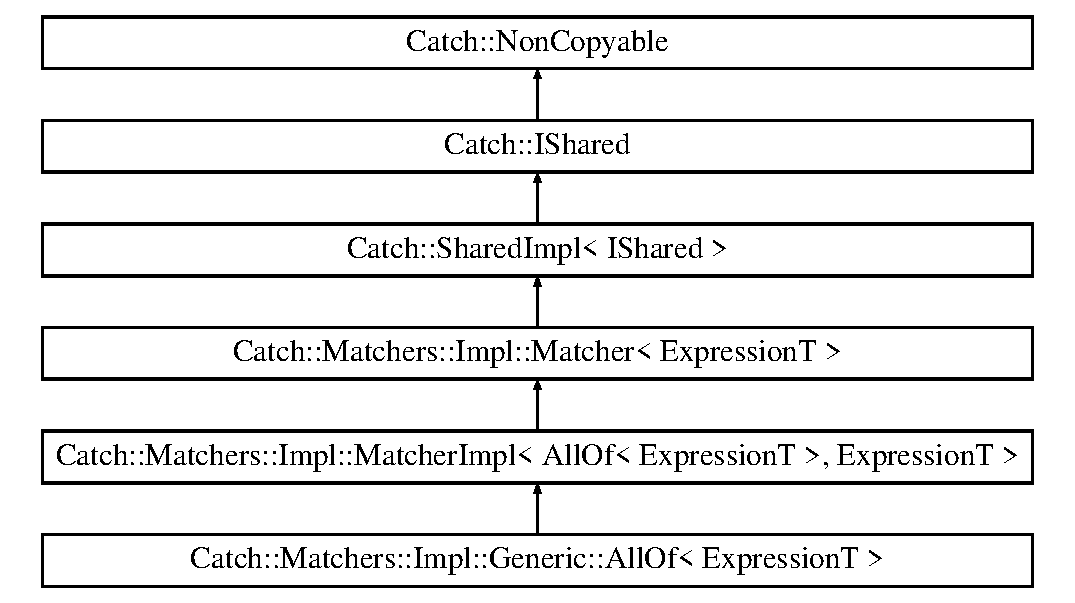
\includegraphics[height=6.000000cm]{classCatch_1_1Matchers_1_1Impl_1_1Generic_1_1AllOf}
\end{center}
\end{figure}
\subsection*{Public Member Functions}
\begin{DoxyCompactItemize}
\item 
{\bfseries All\+Of} (\hyperlink{classCatch_1_1Matchers_1_1Impl_1_1Generic_1_1AllOf}{All\+Of} const \&other)\hypertarget{classCatch_1_1Matchers_1_1Impl_1_1Generic_1_1AllOf_a31f7c5e570e79bdf64064ee87c331a59}{}\label{classCatch_1_1Matchers_1_1Impl_1_1Generic_1_1AllOf_a31f7c5e570e79bdf64064ee87c331a59}

\item 
\hyperlink{classCatch_1_1Matchers_1_1Impl_1_1Generic_1_1AllOf}{All\+Of} \& {\bfseries add} (\hyperlink{structCatch_1_1Matchers_1_1Impl_1_1Matcher}{Matcher}$<$ ExpressionT $>$ const \&matcher)\hypertarget{classCatch_1_1Matchers_1_1Impl_1_1Generic_1_1AllOf_a8c5cd1e494ab697076da418ee72ac297}{}\label{classCatch_1_1Matchers_1_1Impl_1_1Generic_1_1AllOf_a8c5cd1e494ab697076da418ee72ac297}

\item 
virtual bool {\bfseries match} (ExpressionT const \&expr) const \hypertarget{classCatch_1_1Matchers_1_1Impl_1_1Generic_1_1AllOf_a04534d0ac9e089f4500c3c19054f11ce}{}\label{classCatch_1_1Matchers_1_1Impl_1_1Generic_1_1AllOf_a04534d0ac9e089f4500c3c19054f11ce}

\item 
virtual std\+::string {\bfseries to\+String} () const \hypertarget{classCatch_1_1Matchers_1_1Impl_1_1Generic_1_1AllOf_a9febc1e67acbeff62a32bcbfdc0c8fab}{}\label{classCatch_1_1Matchers_1_1Impl_1_1Generic_1_1AllOf_a9febc1e67acbeff62a32bcbfdc0c8fab}

\item 
\hyperlink{classCatch_1_1Matchers_1_1Impl_1_1Generic_1_1AllOf}{All\+Of} {\bfseries operator\&\&} (\hyperlink{structCatch_1_1Matchers_1_1Impl_1_1Matcher}{Matcher}$<$ ExpressionT $>$ const \&other) const \hypertarget{classCatch_1_1Matchers_1_1Impl_1_1Generic_1_1AllOf_ac2b4045ae39746852a0f603715ba1387}{}\label{classCatch_1_1Matchers_1_1Impl_1_1Generic_1_1AllOf_ac2b4045ae39746852a0f603715ba1387}

\end{DoxyCompactItemize}
\subsection*{Additional Inherited Members}


The documentation for this class was generated from the following file\+:\begin{DoxyCompactItemize}
\item 
catch.\+hpp\end{DoxyCompactItemize}

\hypertarget{classCatch_1_1Matchers_1_1Impl_1_1Generic_1_1AnyOf}{}\section{Catch\+:\+:Matchers\+:\+:Impl\+:\+:Generic\+:\+:Any\+Of$<$ ExpressionT $>$ Class Template Reference}
\label{classCatch_1_1Matchers_1_1Impl_1_1Generic_1_1AnyOf}\index{Catch\+::\+Matchers\+::\+Impl\+::\+Generic\+::\+Any\+Of$<$ Expression\+T $>$@{Catch\+::\+Matchers\+::\+Impl\+::\+Generic\+::\+Any\+Of$<$ Expression\+T $>$}}
Inheritance diagram for Catch\+:\+:Matchers\+:\+:Impl\+:\+:Generic\+:\+:Any\+Of$<$ ExpressionT $>$\+:\begin{figure}[H]
\begin{center}
\leavevmode
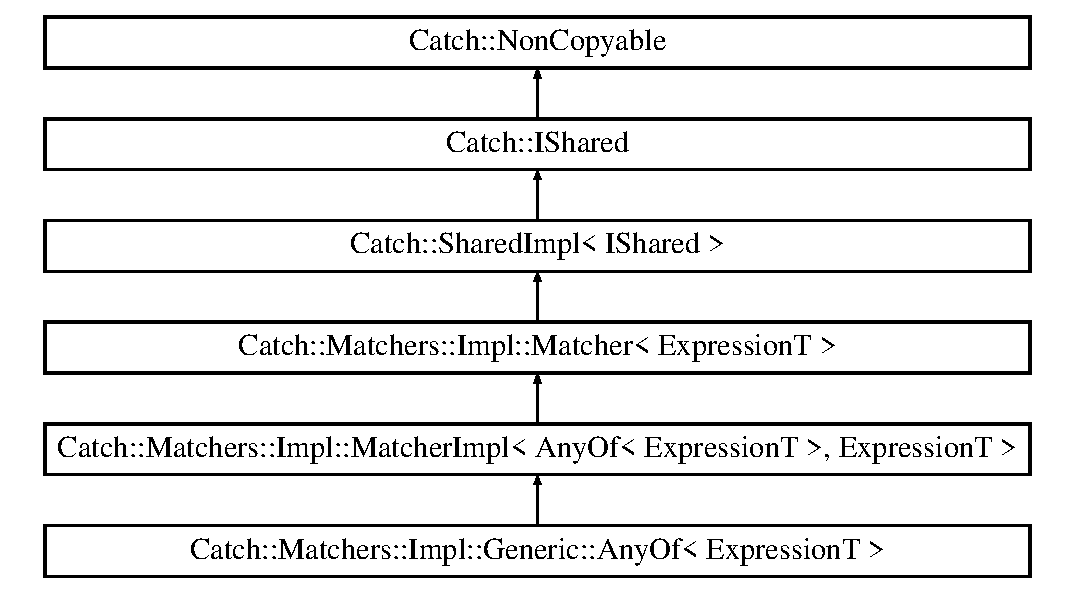
\includegraphics[height=6.000000cm]{classCatch_1_1Matchers_1_1Impl_1_1Generic_1_1AnyOf}
\end{center}
\end{figure}
\subsection*{Public Member Functions}
\begin{DoxyCompactItemize}
\item 
{\bfseries Any\+Of} (\hyperlink{classCatch_1_1Matchers_1_1Impl_1_1Generic_1_1AnyOf}{Any\+Of} const \&other)\hypertarget{classCatch_1_1Matchers_1_1Impl_1_1Generic_1_1AnyOf_a74fbc05b32d334fcbfd0fae0163a404e}{}\label{classCatch_1_1Matchers_1_1Impl_1_1Generic_1_1AnyOf_a74fbc05b32d334fcbfd0fae0163a404e}

\item 
\hyperlink{classCatch_1_1Matchers_1_1Impl_1_1Generic_1_1AnyOf}{Any\+Of} \& {\bfseries add} (\hyperlink{structCatch_1_1Matchers_1_1Impl_1_1Matcher}{Matcher}$<$ ExpressionT $>$ const \&matcher)\hypertarget{classCatch_1_1Matchers_1_1Impl_1_1Generic_1_1AnyOf_a3bce94b627551e5f96c5f9c6060413f0}{}\label{classCatch_1_1Matchers_1_1Impl_1_1Generic_1_1AnyOf_a3bce94b627551e5f96c5f9c6060413f0}

\item 
virtual bool {\bfseries match} (ExpressionT const \&expr) const \hypertarget{classCatch_1_1Matchers_1_1Impl_1_1Generic_1_1AnyOf_a2f97a08338e12deba541043a57d73db9}{}\label{classCatch_1_1Matchers_1_1Impl_1_1Generic_1_1AnyOf_a2f97a08338e12deba541043a57d73db9}

\item 
virtual std\+::string {\bfseries to\+String} () const \hypertarget{classCatch_1_1Matchers_1_1Impl_1_1Generic_1_1AnyOf_a7ecc6ec08b2018a643923a9d450aa328}{}\label{classCatch_1_1Matchers_1_1Impl_1_1Generic_1_1AnyOf_a7ecc6ec08b2018a643923a9d450aa328}

\item 
\hyperlink{classCatch_1_1Matchers_1_1Impl_1_1Generic_1_1AnyOf}{Any\+Of} {\bfseries operator$\vert$$\vert$} (\hyperlink{structCatch_1_1Matchers_1_1Impl_1_1Matcher}{Matcher}$<$ ExpressionT $>$ const \&other) const \hypertarget{classCatch_1_1Matchers_1_1Impl_1_1Generic_1_1AnyOf_a07f4ea2ae366a6521a5d7bff4522e8bf}{}\label{classCatch_1_1Matchers_1_1Impl_1_1Generic_1_1AnyOf_a07f4ea2ae366a6521a5d7bff4522e8bf}

\end{DoxyCompactItemize}
\subsection*{Additional Inherited Members}


The documentation for this class was generated from the following file\+:\begin{DoxyCompactItemize}
\item 
catch.\+hpp\end{DoxyCompactItemize}

\hypertarget{classCatch_1_1Detail_1_1Approx}{}\section{Catch\+:\+:Detail\+:\+:Approx Class Reference}
\label{classCatch_1_1Detail_1_1Approx}\index{Catch\+::\+Detail\+::\+Approx@{Catch\+::\+Detail\+::\+Approx}}
\subsection*{Public Member Functions}
\begin{DoxyCompactItemize}
\item 
{\bfseries Approx} (double value)\hypertarget{classCatch_1_1Detail_1_1Approx_a1a8618ea8db08c66bd3d9fe8f74b957a}{}\label{classCatch_1_1Detail_1_1Approx_a1a8618ea8db08c66bd3d9fe8f74b957a}

\item 
{\bfseries Approx} (\hyperlink{classCatch_1_1Detail_1_1Approx}{Approx} const \&other)\hypertarget{classCatch_1_1Detail_1_1Approx_a807330c63266fc914abdf6e461255a54}{}\label{classCatch_1_1Detail_1_1Approx_a807330c63266fc914abdf6e461255a54}

\item 
\hyperlink{classCatch_1_1Detail_1_1Approx}{Approx} {\bfseries operator()} (double value)\hypertarget{classCatch_1_1Detail_1_1Approx_a48c9cbc28a05dc9dc8c3973b9eae2268}{}\label{classCatch_1_1Detail_1_1Approx_a48c9cbc28a05dc9dc8c3973b9eae2268}

\item 
\hyperlink{classCatch_1_1Detail_1_1Approx}{Approx} \& {\bfseries epsilon} (double new\+Epsilon)\hypertarget{classCatch_1_1Detail_1_1Approx_a05c50c3ad0a971fab19345b5d94979a9}{}\label{classCatch_1_1Detail_1_1Approx_a05c50c3ad0a971fab19345b5d94979a9}

\item 
\hyperlink{classCatch_1_1Detail_1_1Approx}{Approx} \& {\bfseries scale} (double new\+Scale)\hypertarget{classCatch_1_1Detail_1_1Approx_acd80f0737bf38112beacd5ca95bef113}{}\label{classCatch_1_1Detail_1_1Approx_acd80f0737bf38112beacd5ca95bef113}

\item 
std\+::string {\bfseries to\+String} () const \hypertarget{classCatch_1_1Detail_1_1Approx_adeb74b73506b3f6b2ba72aea15168fbe}{}\label{classCatch_1_1Detail_1_1Approx_adeb74b73506b3f6b2ba72aea15168fbe}

\end{DoxyCompactItemize}
\subsection*{Static Public Member Functions}
\begin{DoxyCompactItemize}
\item 
static \hyperlink{classCatch_1_1Detail_1_1Approx}{Approx} {\bfseries custom} ()\hypertarget{classCatch_1_1Detail_1_1Approx_aaf86dc0ee92272ac2d9839197a07951d}{}\label{classCatch_1_1Detail_1_1Approx_aaf86dc0ee92272ac2d9839197a07951d}

\end{DoxyCompactItemize}
\subsection*{Friends}
\begin{DoxyCompactItemize}
\item 
bool {\bfseries operator==} (double lhs, \hyperlink{classCatch_1_1Detail_1_1Approx}{Approx} const \&rhs)\hypertarget{classCatch_1_1Detail_1_1Approx_ac766f044f1c63f0c5997982baefd9049}{}\label{classCatch_1_1Detail_1_1Approx_ac766f044f1c63f0c5997982baefd9049}

\item 
bool {\bfseries operator==} (\hyperlink{classCatch_1_1Detail_1_1Approx}{Approx} const \&lhs, double rhs)\hypertarget{classCatch_1_1Detail_1_1Approx_a35999631e6cef569f9da9f3fa910db22}{}\label{classCatch_1_1Detail_1_1Approx_a35999631e6cef569f9da9f3fa910db22}

\item 
bool {\bfseries operator!=} (double lhs, \hyperlink{classCatch_1_1Detail_1_1Approx}{Approx} const \&rhs)\hypertarget{classCatch_1_1Detail_1_1Approx_a83b3763569a7ecc143c335b630be0e47}{}\label{classCatch_1_1Detail_1_1Approx_a83b3763569a7ecc143c335b630be0e47}

\item 
bool {\bfseries operator!=} (\hyperlink{classCatch_1_1Detail_1_1Approx}{Approx} const \&lhs, double rhs)\hypertarget{classCatch_1_1Detail_1_1Approx_a7497ef839f8026cc0edd6269a80f3e09}{}\label{classCatch_1_1Detail_1_1Approx_a7497ef839f8026cc0edd6269a80f3e09}

\end{DoxyCompactItemize}


The documentation for this class was generated from the following file\+:\begin{DoxyCompactItemize}
\item 
catch.\+hpp\end{DoxyCompactItemize}

\hypertarget{structCatch_1_1AssertionInfo}{}\section{Catch\+:\+:Assertion\+Info Struct Reference}
\label{structCatch_1_1AssertionInfo}\index{Catch\+::\+Assertion\+Info@{Catch\+::\+Assertion\+Info}}
\subsection*{Public Member Functions}
\begin{DoxyCompactItemize}
\item 
{\bfseries Assertion\+Info} (std\+::string const \&\+\_\+macro\+Name, \hyperlink{structCatch_1_1SourceLineInfo}{Source\+Line\+Info} const \&\+\_\+line\+Info, std\+::string const \&\+\_\+captured\+Expression, Result\+Disposition\+::\+Flags \+\_\+result\+Disposition)\hypertarget{structCatch_1_1AssertionInfo_aaf6cc3eebd40391e54d37ed42953c73f}{}\label{structCatch_1_1AssertionInfo_aaf6cc3eebd40391e54d37ed42953c73f}

\end{DoxyCompactItemize}
\subsection*{Public Attributes}
\begin{DoxyCompactItemize}
\item 
std\+::string {\bfseries macro\+Name}\hypertarget{structCatch_1_1AssertionInfo_ac2e59e8c89e00eb3390768f50d540b18}{}\label{structCatch_1_1AssertionInfo_ac2e59e8c89e00eb3390768f50d540b18}

\item 
\hyperlink{structCatch_1_1SourceLineInfo}{Source\+Line\+Info} {\bfseries line\+Info}\hypertarget{structCatch_1_1AssertionInfo_a17bdbb404ba12658034f833be2f4c3e7}{}\label{structCatch_1_1AssertionInfo_a17bdbb404ba12658034f833be2f4c3e7}

\item 
std\+::string {\bfseries captured\+Expression}\hypertarget{structCatch_1_1AssertionInfo_af7c1d3cbfa346e9a303030fa0ef0cb54}{}\label{structCatch_1_1AssertionInfo_af7c1d3cbfa346e9a303030fa0ef0cb54}

\item 
Result\+Disposition\+::\+Flags {\bfseries result\+Disposition}\hypertarget{structCatch_1_1AssertionInfo_a60353b3632ab2f827162f2b2d6911073}{}\label{structCatch_1_1AssertionInfo_a60353b3632ab2f827162f2b2d6911073}

\end{DoxyCompactItemize}


The documentation for this struct was generated from the following file\+:\begin{DoxyCompactItemize}
\item 
catch.\+hpp\end{DoxyCompactItemize}

\hypertarget{classCatch_1_1AssertionResult}{}\section{Catch\+:\+:Assertion\+Result Class Reference}
\label{classCatch_1_1AssertionResult}\index{Catch\+::\+Assertion\+Result@{Catch\+::\+Assertion\+Result}}
\subsection*{Public Member Functions}
\begin{DoxyCompactItemize}
\item 
{\bfseries Assertion\+Result} (\hyperlink{structCatch_1_1AssertionInfo}{Assertion\+Info} const \&info, \hyperlink{structCatch_1_1AssertionResultData}{Assertion\+Result\+Data} const \&data)\hypertarget{classCatch_1_1AssertionResult_ab58aeec27052ba400633ed0e36cea692}{}\label{classCatch_1_1AssertionResult_ab58aeec27052ba400633ed0e36cea692}

\item 
bool {\bfseries is\+Ok} () const \hypertarget{classCatch_1_1AssertionResult_a70fb6aa62a38db3bdcafb4bb134afb21}{}\label{classCatch_1_1AssertionResult_a70fb6aa62a38db3bdcafb4bb134afb21}

\item 
bool {\bfseries succeeded} () const \hypertarget{classCatch_1_1AssertionResult_a5404062147930354afeb154de7cbaa7e}{}\label{classCatch_1_1AssertionResult_a5404062147930354afeb154de7cbaa7e}

\item 
Result\+Was\+::\+Of\+Type {\bfseries get\+Result\+Type} () const \hypertarget{classCatch_1_1AssertionResult_aa90bec8064879a62fcdc8e1079bcdba1}{}\label{classCatch_1_1AssertionResult_aa90bec8064879a62fcdc8e1079bcdba1}

\item 
bool {\bfseries has\+Expression} () const \hypertarget{classCatch_1_1AssertionResult_a45551f4f092c640ffce0cdd8a94f4b62}{}\label{classCatch_1_1AssertionResult_a45551f4f092c640ffce0cdd8a94f4b62}

\item 
bool {\bfseries has\+Message} () const \hypertarget{classCatch_1_1AssertionResult_ab22a1c9baa182aeb2549fffeb8294d9e}{}\label{classCatch_1_1AssertionResult_ab22a1c9baa182aeb2549fffeb8294d9e}

\item 
std\+::string {\bfseries get\+Expression} () const \hypertarget{classCatch_1_1AssertionResult_a6105300b90d66b5c11b69813f83d074d}{}\label{classCatch_1_1AssertionResult_a6105300b90d66b5c11b69813f83d074d}

\item 
std\+::string {\bfseries get\+Expression\+In\+Macro} () const \hypertarget{classCatch_1_1AssertionResult_ac368a7490af7669decd58efea7d7dc54}{}\label{classCatch_1_1AssertionResult_ac368a7490af7669decd58efea7d7dc54}

\item 
bool {\bfseries has\+Expanded\+Expression} () const \hypertarget{classCatch_1_1AssertionResult_a122c369bd49430a304e3eaebdf184f36}{}\label{classCatch_1_1AssertionResult_a122c369bd49430a304e3eaebdf184f36}

\item 
std\+::string {\bfseries get\+Expanded\+Expression} () const \hypertarget{classCatch_1_1AssertionResult_a675d074588875eb62b0b6e36e05d65e6}{}\label{classCatch_1_1AssertionResult_a675d074588875eb62b0b6e36e05d65e6}

\item 
std\+::string {\bfseries get\+Message} () const \hypertarget{classCatch_1_1AssertionResult_a9793bfc4d24678c8a013bda84a5aa905}{}\label{classCatch_1_1AssertionResult_a9793bfc4d24678c8a013bda84a5aa905}

\item 
\hyperlink{structCatch_1_1SourceLineInfo}{Source\+Line\+Info} {\bfseries get\+Source\+Info} () const \hypertarget{classCatch_1_1AssertionResult_a68b73fe982a97fe6432af679af1a2dad}{}\label{classCatch_1_1AssertionResult_a68b73fe982a97fe6432af679af1a2dad}

\item 
std\+::string {\bfseries get\+Test\+Macro\+Name} () const \hypertarget{classCatch_1_1AssertionResult_a2901d41b199258ff6a44571b147169dd}{}\label{classCatch_1_1AssertionResult_a2901d41b199258ff6a44571b147169dd}

\end{DoxyCompactItemize}
\subsection*{Protected Attributes}
\begin{DoxyCompactItemize}
\item 
\hyperlink{structCatch_1_1AssertionInfo}{Assertion\+Info} {\bfseries m\+\_\+info}\hypertarget{classCatch_1_1AssertionResult_a3e7236f73a51d6fc8bb9dfdefcee7772}{}\label{classCatch_1_1AssertionResult_a3e7236f73a51d6fc8bb9dfdefcee7772}

\item 
\hyperlink{structCatch_1_1AssertionResultData}{Assertion\+Result\+Data} {\bfseries m\+\_\+result\+Data}\hypertarget{classCatch_1_1AssertionResult_add3455b8bbedb0d643e18da67c66b4f7}{}\label{classCatch_1_1AssertionResult_add3455b8bbedb0d643e18da67c66b4f7}

\end{DoxyCompactItemize}


The documentation for this class was generated from the following file\+:\begin{DoxyCompactItemize}
\item 
catch.\+hpp\end{DoxyCompactItemize}

\hypertarget{structCatch_1_1AssertionResultData}{}\section{Catch\+:\+:Assertion\+Result\+Data Struct Reference}
\label{structCatch_1_1AssertionResultData}\index{Catch\+::\+Assertion\+Result\+Data@{Catch\+::\+Assertion\+Result\+Data}}
\subsection*{Public Attributes}
\begin{DoxyCompactItemize}
\item 
std\+::string {\bfseries reconstructed\+Expression}\hypertarget{structCatch_1_1AssertionResultData_a9e809d36fffbeb1c7d0cbe7382dd9595}{}\label{structCatch_1_1AssertionResultData_a9e809d36fffbeb1c7d0cbe7382dd9595}

\item 
std\+::string {\bfseries message}\hypertarget{structCatch_1_1AssertionResultData_ac34215803c4c4a88f795879f61c1f7b4}{}\label{structCatch_1_1AssertionResultData_ac34215803c4c4a88f795879f61c1f7b4}

\item 
Result\+Was\+::\+Of\+Type {\bfseries result\+Type}\hypertarget{structCatch_1_1AssertionResultData_a7ceab4a7ff722aec5587e3748caf66b7}{}\label{structCatch_1_1AssertionResultData_a7ceab4a7ff722aec5587e3748caf66b7}

\end{DoxyCompactItemize}


The documentation for this struct was generated from the following file\+:\begin{DoxyCompactItemize}
\item 
catch.\+hpp\end{DoxyCompactItemize}

\hypertarget{structCatch_1_1AutoReg}{}\section{Catch\+:\+:Auto\+Reg Struct Reference}
\label{structCatch_1_1AutoReg}\index{Catch\+::\+Auto\+Reg@{Catch\+::\+Auto\+Reg}}
\subsection*{Public Member Functions}
\begin{DoxyCompactItemize}
\item 
{\bfseries Auto\+Reg} (Test\+Function function, \hyperlink{structCatch_1_1SourceLineInfo}{Source\+Line\+Info} const \&line\+Info, \hyperlink{structCatch_1_1NameAndDesc}{Name\+And\+Desc} const \&name\+And\+Desc)\hypertarget{structCatch_1_1AutoReg_af224f4568d57b8652474df475a164a8c}{}\label{structCatch_1_1AutoReg_af224f4568d57b8652474df475a164a8c}

\item 
{\footnotesize template$<$typename C $>$ }\\{\bfseries Auto\+Reg} (void(C\+::$\ast$method)(), char const $\ast$class\+Name, \hyperlink{structCatch_1_1NameAndDesc}{Name\+And\+Desc} const \&name\+And\+Desc, \hyperlink{structCatch_1_1SourceLineInfo}{Source\+Line\+Info} const \&line\+Info)\hypertarget{structCatch_1_1AutoReg_a1bf9207fe0a02b46dc0ab1cc03cbe738}{}\label{structCatch_1_1AutoReg_a1bf9207fe0a02b46dc0ab1cc03cbe738}

\end{DoxyCompactItemize}


The documentation for this struct was generated from the following file\+:\begin{DoxyCompactItemize}
\item 
catch.\+hpp\end{DoxyCompactItemize}

\hypertarget{classCatch_1_1BetweenGenerator}{}\section{Catch\+:\+:Between\+Generator$<$ T $>$ Class Template Reference}
\label{classCatch_1_1BetweenGenerator}\index{Catch\+::\+Between\+Generator$<$ T $>$@{Catch\+::\+Between\+Generator$<$ T $>$}}
Inheritance diagram for Catch\+:\+:Between\+Generator$<$ T $>$\+:\begin{figure}[H]
\begin{center}
\leavevmode
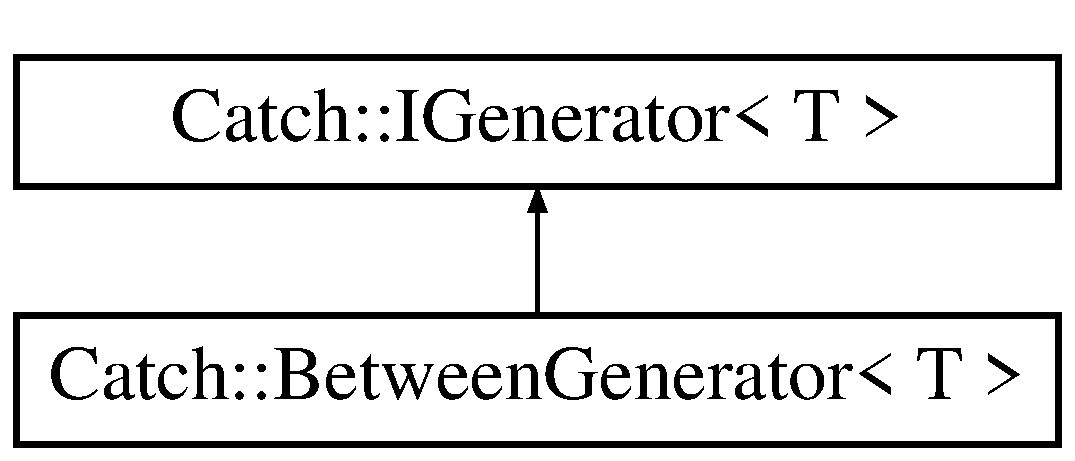
\includegraphics[height=2.000000cm]{classCatch_1_1BetweenGenerator}
\end{center}
\end{figure}
\subsection*{Public Member Functions}
\begin{DoxyCompactItemize}
\item 
{\bfseries Between\+Generator} (T from, T to)\hypertarget{classCatch_1_1BetweenGenerator_a835a057d691ae37caef660624099b51c}{}\label{classCatch_1_1BetweenGenerator_a835a057d691ae37caef660624099b51c}

\item 
virtual T {\bfseries get\+Value} (std\+::size\+\_\+t index) const \hypertarget{classCatch_1_1BetweenGenerator_af83575d62cc727ca995446cff4d6c26c}{}\label{classCatch_1_1BetweenGenerator_af83575d62cc727ca995446cff4d6c26c}

\item 
virtual std\+::size\+\_\+t {\bfseries size} () const \hypertarget{classCatch_1_1BetweenGenerator_aa53a04a259e796ba2b5adabed79474b5}{}\label{classCatch_1_1BetweenGenerator_aa53a04a259e796ba2b5adabed79474b5}

\end{DoxyCompactItemize}


The documentation for this class was generated from the following file\+:\begin{DoxyCompactItemize}
\item 
catch.\+hpp\end{DoxyCompactItemize}

\hypertarget{classBoard}{}\section{Board Class Reference}
\label{classBoard}\index{Board@{Board}}
\subsection*{Public Member Functions}
\begin{DoxyCompactItemize}
\item 
bool {\bfseries is\+Occupied} ()\hypertarget{classBoard_a81a02ad38ac196b01247dee0405dacad}{}\label{classBoard_a81a02ad38ac196b01247dee0405dacad}

\item 
bool {\bfseries is\+Primary} ()\hypertarget{classBoard_abda639fefd04286773bf2f99e57f3437}{}\label{classBoard_abda639fefd04286773bf2f99e57f3437}

\item 
int {\bfseries get\+Size} ()\hypertarget{classBoard_af093d8ac43989ad95dc03c714335b8e5}{}\label{classBoard_af093d8ac43989ad95dc03c714335b8e5}

\item 
void {\bfseries set\+Size} (int size)\hypertarget{classBoard_a3bed92eb3da5c865cf591292631c9353}{}\label{classBoard_a3bed92eb3da5c865cf591292631c9353}

\item 
int {\bfseries total\+Cells} ()\hypertarget{classBoard_af0ae9fa40ac726469140bab4f051a790}{}\label{classBoard_af0ae9fa40ac726469140bab4f051a790}

\item 
void {\bfseries set\+Head} (int, int)\hypertarget{classBoard_a730a16434b08168d0d927dc56331d473}{}\label{classBoard_a730a16434b08168d0d927dc56331d473}

\item 
void {\bfseries set\+Occupied} (int, int)\hypertarget{classBoard_aa3cb6d8c9451c37597f69b3c37453994}{}\label{classBoard_aa3cb6d8c9451c37597f69b3c37453994}

\item 
bool {\bfseries is\+Head} (int, int)\hypertarget{classBoard_acc1408df43b2b1d616fb3d2b84667336}{}\label{classBoard_acc1408df43b2b1d616fb3d2b84667336}

\item 
bool {\bfseries is\+Occupied} (int, int)\hypertarget{classBoard_ad1a7a95b25a3725fdc36b7f18afd1e22}{}\label{classBoard_ad1a7a95b25a3725fdc36b7f18afd1e22}

\item 
{\bfseries Board} (int size, bool is\+Primary)\hypertarget{classBoard_a13cc3e8fad90e23e2826edcc690c2ce1}{}\label{classBoard_a13cc3e8fad90e23e2826edcc690c2ce1}

\end{DoxyCompactItemize}
\subsection*{Public Attributes}
\begin{DoxyCompactItemize}
\item 
vector$<$ vector$<$ \hyperlink{classCell}{Cell} $>$ $>$ {\bfseries board\+\_\+}\hypertarget{classBoard_a85f83047c4d44bbb16704e7bd0970cd0}{}\label{classBoard_a85f83047c4d44bbb16704e7bd0970cd0}

\end{DoxyCompactItemize}


The documentation for this class was generated from the following files\+:\begin{DoxyCompactItemize}
\item 
Board.\+h\item 
Board.\+cpp\end{DoxyCompactItemize}

\hypertarget{structCatch_1_1Detail_1_1BorgType}{}\section{Catch\+:\+:Detail\+:\+:Borg\+Type Struct Reference}
\label{structCatch_1_1Detail_1_1BorgType}\index{Catch\+::\+Detail\+::\+Borg\+Type@{Catch\+::\+Detail\+::\+Borg\+Type}}
\subsection*{Public Member Functions}
\begin{DoxyCompactItemize}
\item 
{\footnotesize template$<$typename T $>$ }\\{\bfseries Borg\+Type} (T const \&)\hypertarget{structCatch_1_1Detail_1_1BorgType_a780a9946ed0d654f0bfc043c8fc505d8}{}\label{structCatch_1_1Detail_1_1BorgType_a780a9946ed0d654f0bfc043c8fc505d8}

\end{DoxyCompactItemize}


The documentation for this struct was generated from the following file\+:\begin{DoxyCompactItemize}
\item 
catch.\+hpp\end{DoxyCompactItemize}

\hypertarget{structCatch_1_1Matchers_1_1Impl_1_1StdString_1_1CasedString}{}\section{Catch\+:\+:Matchers\+:\+:Impl\+:\+:Std\+String\+:\+:Cased\+String Struct Reference}
\label{structCatch_1_1Matchers_1_1Impl_1_1StdString_1_1CasedString}\index{Catch\+::\+Matchers\+::\+Impl\+::\+Std\+String\+::\+Cased\+String@{Catch\+::\+Matchers\+::\+Impl\+::\+Std\+String\+::\+Cased\+String}}
\subsection*{Public Member Functions}
\begin{DoxyCompactItemize}
\item 
{\bfseries Cased\+String} (std\+::string const \&str, Case\+Sensitive\+::\+Choice case\+Sensitivity)\hypertarget{structCatch_1_1Matchers_1_1Impl_1_1StdString_1_1CasedString_aebd017c88423d8a11c62cff85754a22d}{}\label{structCatch_1_1Matchers_1_1Impl_1_1StdString_1_1CasedString_aebd017c88423d8a11c62cff85754a22d}

\item 
std\+::string {\bfseries adjust\+String} (std\+::string const \&str) const \hypertarget{structCatch_1_1Matchers_1_1Impl_1_1StdString_1_1CasedString_aaf5c4be8b3b8b317777d0e332d3733b5}{}\label{structCatch_1_1Matchers_1_1Impl_1_1StdString_1_1CasedString_aaf5c4be8b3b8b317777d0e332d3733b5}

\item 
std\+::string {\bfseries to\+String\+Suffix} () const \hypertarget{structCatch_1_1Matchers_1_1Impl_1_1StdString_1_1CasedString_ae5865fa1dd20c80498a094cae5459883}{}\label{structCatch_1_1Matchers_1_1Impl_1_1StdString_1_1CasedString_ae5865fa1dd20c80498a094cae5459883}

\end{DoxyCompactItemize}
\subsection*{Public Attributes}
\begin{DoxyCompactItemize}
\item 
Case\+Sensitive\+::\+Choice {\bfseries m\+\_\+case\+Sensitivity}\hypertarget{structCatch_1_1Matchers_1_1Impl_1_1StdString_1_1CasedString_af399ed93051d8981e298206dee6898b3}{}\label{structCatch_1_1Matchers_1_1Impl_1_1StdString_1_1CasedString_af399ed93051d8981e298206dee6898b3}

\item 
std\+::string {\bfseries m\+\_\+str}\hypertarget{structCatch_1_1Matchers_1_1Impl_1_1StdString_1_1CasedString_a9f8ce063a934330ac59bf8638f047e99}{}\label{structCatch_1_1Matchers_1_1Impl_1_1StdString_1_1CasedString_a9f8ce063a934330ac59bf8638f047e99}

\end{DoxyCompactItemize}


The documentation for this struct was generated from the following file\+:\begin{DoxyCompactItemize}
\item 
catch.\+hpp\end{DoxyCompactItemize}

\hypertarget{structCatch_1_1CaseSensitive}{}\section{Catch\+:\+:Case\+Sensitive Struct Reference}
\label{structCatch_1_1CaseSensitive}\index{Catch\+::\+Case\+Sensitive@{Catch\+::\+Case\+Sensitive}}
\subsection*{Public Types}
\begin{DoxyCompactItemize}
\item 
enum {\bfseries Choice} \{ {\bfseries Yes}, 
{\bfseries No}
 \}\hypertarget{structCatch_1_1CaseSensitive_aad49d3aee2d97066642fffa919685c6a}{}\label{structCatch_1_1CaseSensitive_aad49d3aee2d97066642fffa919685c6a}

\end{DoxyCompactItemize}


The documentation for this struct was generated from the following file\+:\begin{DoxyCompactItemize}
\item 
catch.\+hpp\end{DoxyCompactItemize}

\hypertarget{classCell}{}\section{Cell Class Reference}
\label{classCell}\index{Cell@{Cell}}
\subsection*{Public Member Functions}
\begin{DoxyCompactItemize}
\item 
bool {\bfseries is\+Occupied} ()\hypertarget{classCell_a5f18a8962841567498aec286d23f153c}{}\label{classCell_a5f18a8962841567498aec286d23f153c}

\item 
bool {\bfseries is\+Head} ()\hypertarget{classCell_a071d12e8c85897affa572e71f681b7ab}{}\label{classCell_a071d12e8c85897affa572e71f681b7ab}

\item 
void {\bfseries set\+Occupied} ()\hypertarget{classCell_a4c6f53c6da9c60f6389873a50ce9d206}{}\label{classCell_a4c6f53c6da9c60f6389873a50ce9d206}

\item 
void {\bfseries set\+Head} ()\hypertarget{classCell_a94f6061a611acdee0a8eac2cbffd4e99}{}\label{classCell_a94f6061a611acdee0a8eac2cbffd4e99}

\item 
tuple$<$ float, float, float, float $>$ {\bfseries get\+Bounds} ()\hypertarget{classCell_a9ba09bf14fe823ba830e134febdd8301}{}\label{classCell_a9ba09bf14fe823ba830e134febdd8301}

\item 
void {\bfseries set\+Bounds} (float, float, float, float)\hypertarget{classCell_a743b44fced5dac88229c9533a604fc10}{}\label{classCell_a743b44fced5dac88229c9533a604fc10}

\item 
bool {\bfseries get\+Square\+Hover} ()\hypertarget{classCell_afe7e2092a8d2eb880c29c1729c9f3656}{}\label{classCell_afe7e2092a8d2eb880c29c1729c9f3656}

\item 
void {\bfseries set\+Square\+Hover} (bool)\hypertarget{classCell_a7fa0f371355d415799f833b1a17c699f}{}\label{classCell_a7fa0f371355d415799f833b1a17c699f}

\end{DoxyCompactItemize}


The documentation for this class was generated from the following files\+:\begin{DoxyCompactItemize}
\item 
Cell.\+h\item 
Cell.\+cpp\end{DoxyCompactItemize}

\hypertarget{classCatch_1_1CompositeGenerator}{}\section{Catch\+:\+:Composite\+Generator$<$ T $>$ Class Template Reference}
\label{classCatch_1_1CompositeGenerator}\index{Catch\+::\+Composite\+Generator$<$ T $>$@{Catch\+::\+Composite\+Generator$<$ T $>$}}
\subsection*{Public Member Functions}
\begin{DoxyCompactItemize}
\item 
{\bfseries Composite\+Generator} (\hyperlink{classCatch_1_1CompositeGenerator}{Composite\+Generator} \&other)\hypertarget{classCatch_1_1CompositeGenerator_a21a7070a00e4a6fe021294c356692692}{}\label{classCatch_1_1CompositeGenerator_a21a7070a00e4a6fe021294c356692692}

\item 
\hyperlink{classCatch_1_1CompositeGenerator}{Composite\+Generator} \& {\bfseries set\+File\+Info} (const char $\ast$file\+Info)\hypertarget{classCatch_1_1CompositeGenerator_ac3c57cf4ca5472f440bf71e2936bcd4a}{}\label{classCatch_1_1CompositeGenerator_ac3c57cf4ca5472f440bf71e2936bcd4a}

\item 
{\bfseries operator T} () const \hypertarget{classCatch_1_1CompositeGenerator_aa3f627d84fb256df0404d19d7fd4b784}{}\label{classCatch_1_1CompositeGenerator_aa3f627d84fb256df0404d19d7fd4b784}

\item 
void {\bfseries add} (const \hyperlink{structCatch_1_1IGenerator}{I\+Generator}$<$ T $>$ $\ast$generator)\hypertarget{classCatch_1_1CompositeGenerator_af3774d42ad2d3453d089ca599efe0517}{}\label{classCatch_1_1CompositeGenerator_af3774d42ad2d3453d089ca599efe0517}

\item 
\hyperlink{classCatch_1_1CompositeGenerator}{Composite\+Generator} \& {\bfseries then} (\hyperlink{classCatch_1_1CompositeGenerator}{Composite\+Generator} \&other)\hypertarget{classCatch_1_1CompositeGenerator_a2e03f42df85cdd238aabd77a80b075d5}{}\label{classCatch_1_1CompositeGenerator_a2e03f42df85cdd238aabd77a80b075d5}

\item 
\hyperlink{classCatch_1_1CompositeGenerator}{Composite\+Generator} \& {\bfseries then} (T value)\hypertarget{classCatch_1_1CompositeGenerator_aefdc11bcfccdf07d2db5f0da3ed8758c}{}\label{classCatch_1_1CompositeGenerator_aefdc11bcfccdf07d2db5f0da3ed8758c}

\end{DoxyCompactItemize}


The documentation for this class was generated from the following file\+:\begin{DoxyCompactItemize}
\item 
catch.\+hpp\end{DoxyCompactItemize}

\hypertarget{structCatch_1_1Matchers_1_1Impl_1_1StdString_1_1Contains}{}\section{Catch\+:\+:Matchers\+:\+:Impl\+:\+:Std\+String\+:\+:Contains Struct Reference}
\label{structCatch_1_1Matchers_1_1Impl_1_1StdString_1_1Contains}\index{Catch\+::\+Matchers\+::\+Impl\+::\+Std\+String\+::\+Contains@{Catch\+::\+Matchers\+::\+Impl\+::\+Std\+String\+::\+Contains}}
Inheritance diagram for Catch\+:\+:Matchers\+:\+:Impl\+:\+:Std\+String\+:\+:Contains\+:\begin{figure}[H]
\begin{center}
\leavevmode
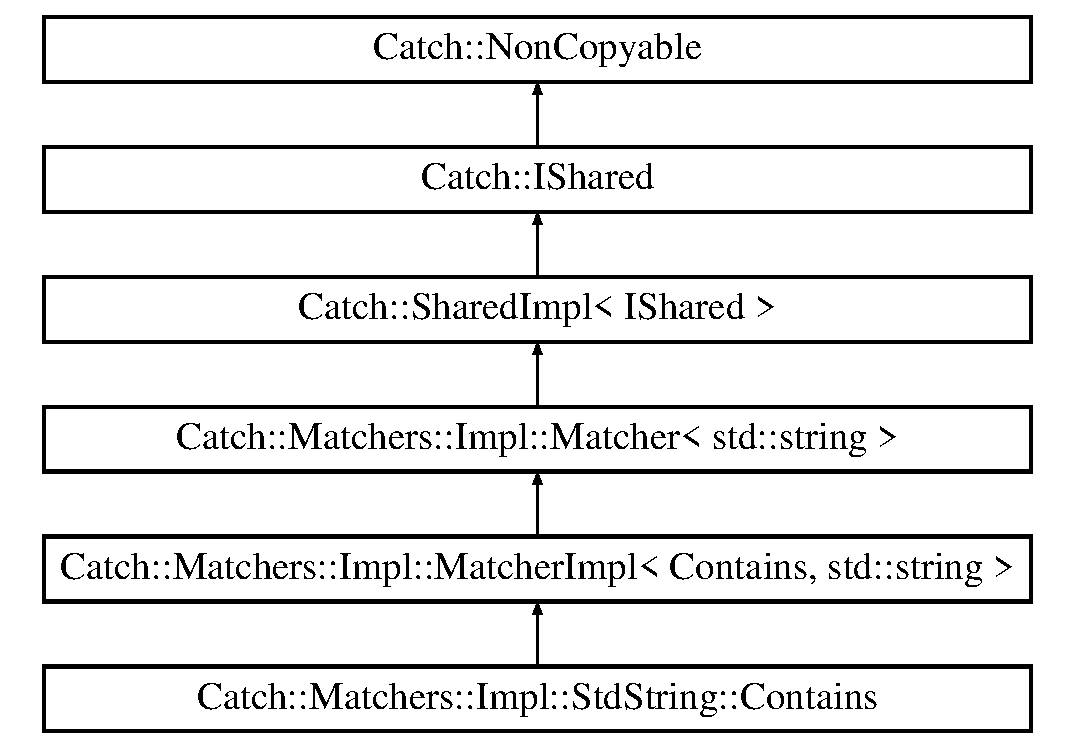
\includegraphics[height=6.000000cm]{structCatch_1_1Matchers_1_1Impl_1_1StdString_1_1Contains}
\end{center}
\end{figure}
\subsection*{Public Member Functions}
\begin{DoxyCompactItemize}
\item 
{\bfseries Contains} (std\+::string const \&substr, Case\+Sensitive\+::\+Choice case\+Sensitivity=Case\+Sensitive\+::\+Yes)\hypertarget{structCatch_1_1Matchers_1_1Impl_1_1StdString_1_1Contains_a7a062d83bd3e3075929dbb55e1c24258}{}\label{structCatch_1_1Matchers_1_1Impl_1_1StdString_1_1Contains_a7a062d83bd3e3075929dbb55e1c24258}

\item 
{\bfseries Contains} (\hyperlink{structCatch_1_1Matchers_1_1Impl_1_1StdString_1_1Contains}{Contains} const \&other)\hypertarget{structCatch_1_1Matchers_1_1Impl_1_1StdString_1_1Contains_ad6b1ef653dfcb3bab43c43be043dc4e8}{}\label{structCatch_1_1Matchers_1_1Impl_1_1StdString_1_1Contains_ad6b1ef653dfcb3bab43c43be043dc4e8}

\item 
virtual bool {\bfseries match} (std\+::string const \&expr) const \hypertarget{structCatch_1_1Matchers_1_1Impl_1_1StdString_1_1Contains_aa27d823dea5770025a24424fc3355a6f}{}\label{structCatch_1_1Matchers_1_1Impl_1_1StdString_1_1Contains_aa27d823dea5770025a24424fc3355a6f}

\item 
virtual std\+::string {\bfseries to\+String} () const \hypertarget{structCatch_1_1Matchers_1_1Impl_1_1StdString_1_1Contains_a226755351f3598179925f3ab89d6def7}{}\label{structCatch_1_1Matchers_1_1Impl_1_1StdString_1_1Contains_a226755351f3598179925f3ab89d6def7}

\end{DoxyCompactItemize}
\subsection*{Public Attributes}
\begin{DoxyCompactItemize}
\item 
\hyperlink{structCatch_1_1Matchers_1_1Impl_1_1StdString_1_1CasedString}{Cased\+String} {\bfseries m\+\_\+data}\hypertarget{structCatch_1_1Matchers_1_1Impl_1_1StdString_1_1Contains_a419a9ecaeaa417d4987982402e08b3eb}{}\label{structCatch_1_1Matchers_1_1Impl_1_1StdString_1_1Contains_a419a9ecaeaa417d4987982402e08b3eb}

\end{DoxyCompactItemize}
\subsection*{Additional Inherited Members}


The documentation for this struct was generated from the following file\+:\begin{DoxyCompactItemize}
\item 
catch.\+hpp\end{DoxyCompactItemize}

\hypertarget{structCatch_1_1CopyableStream}{}\section{Catch\+:\+:Copyable\+Stream Struct Reference}
\label{structCatch_1_1CopyableStream}\index{Catch\+::\+Copyable\+Stream@{Catch\+::\+Copyable\+Stream}}
\subsection*{Public Member Functions}
\begin{DoxyCompactItemize}
\item 
{\bfseries Copyable\+Stream} (\hyperlink{structCatch_1_1CopyableStream}{Copyable\+Stream} const \&other)\hypertarget{structCatch_1_1CopyableStream_a0e72dc16240653f52c17106f4bf34da8}{}\label{structCatch_1_1CopyableStream_a0e72dc16240653f52c17106f4bf34da8}

\item 
\hyperlink{structCatch_1_1CopyableStream}{Copyable\+Stream} \& {\bfseries operator=} (\hyperlink{structCatch_1_1CopyableStream}{Copyable\+Stream} const \&other)\hypertarget{structCatch_1_1CopyableStream_a1760fa29b38011c5845171260bec0966}{}\label{structCatch_1_1CopyableStream_a1760fa29b38011c5845171260bec0966}

\end{DoxyCompactItemize}
\subsection*{Public Attributes}
\begin{DoxyCompactItemize}
\item 
std\+::ostringstream {\bfseries oss}\hypertarget{structCatch_1_1CopyableStream_ae123fb4d673e7d7a13a3c5f6bc5d426c}{}\label{structCatch_1_1CopyableStream_ae123fb4d673e7d7a13a3c5f6bc5d426c}

\end{DoxyCompactItemize}


The documentation for this struct was generated from the following file\+:\begin{DoxyCompactItemize}
\item 
catch.\+hpp\end{DoxyCompactItemize}

\hypertarget{structCatch_1_1Counts}{}\section{Catch\+:\+:Counts Struct Reference}
\label{structCatch_1_1Counts}\index{Catch\+::\+Counts@{Catch\+::\+Counts}}
\subsection*{Public Member Functions}
\begin{DoxyCompactItemize}
\item 
\hyperlink{structCatch_1_1Counts}{Counts} {\bfseries operator-\/} (\hyperlink{structCatch_1_1Counts}{Counts} const \&other) const \hypertarget{structCatch_1_1Counts_aedf86fefe33938d132a6981171cd83e6}{}\label{structCatch_1_1Counts_aedf86fefe33938d132a6981171cd83e6}

\item 
\hyperlink{structCatch_1_1Counts}{Counts} \& {\bfseries operator+=} (\hyperlink{structCatch_1_1Counts}{Counts} const \&other)\hypertarget{structCatch_1_1Counts_a322a89475cd2cc039140ef371e973677}{}\label{structCatch_1_1Counts_a322a89475cd2cc039140ef371e973677}

\item 
std\+::size\+\_\+t {\bfseries total} () const \hypertarget{structCatch_1_1Counts_a9125c662e30114e5c5cc94729b1e9e84}{}\label{structCatch_1_1Counts_a9125c662e30114e5c5cc94729b1e9e84}

\item 
bool {\bfseries all\+Passed} () const \hypertarget{structCatch_1_1Counts_adbbaca552f6017ce69e0d5dc5500bea4}{}\label{structCatch_1_1Counts_adbbaca552f6017ce69e0d5dc5500bea4}

\item 
bool {\bfseries all\+Ok} () const \hypertarget{structCatch_1_1Counts_ab2497c9dfc77be757a90225ea69595f5}{}\label{structCatch_1_1Counts_ab2497c9dfc77be757a90225ea69595f5}

\end{DoxyCompactItemize}
\subsection*{Public Attributes}
\begin{DoxyCompactItemize}
\item 
std\+::size\+\_\+t {\bfseries passed}\hypertarget{structCatch_1_1Counts_ad28daaf3de28006400208b6dd0c631e6}{}\label{structCatch_1_1Counts_ad28daaf3de28006400208b6dd0c631e6}

\item 
std\+::size\+\_\+t {\bfseries failed}\hypertarget{structCatch_1_1Counts_a19982a3817a3bc2c07f0290e71f497a3}{}\label{structCatch_1_1Counts_a19982a3817a3bc2c07f0290e71f497a3}

\item 
std\+::size\+\_\+t {\bfseries failed\+But\+Ok}\hypertarget{structCatch_1_1Counts_ac090973a2ff51394cd452718e75c073e}{}\label{structCatch_1_1Counts_ac090973a2ff51394cd452718e75c073e}

\end{DoxyCompactItemize}


The documentation for this struct was generated from the following file\+:\begin{DoxyCompactItemize}
\item 
catch.\+hpp\end{DoxyCompactItemize}

\hypertarget{structCatch_1_1Matchers_1_1Impl_1_1StdString_1_1EndsWith}{}\section{Catch\+:\+:Matchers\+:\+:Impl\+:\+:Std\+String\+:\+:Ends\+With Struct Reference}
\label{structCatch_1_1Matchers_1_1Impl_1_1StdString_1_1EndsWith}\index{Catch\+::\+Matchers\+::\+Impl\+::\+Std\+String\+::\+Ends\+With@{Catch\+::\+Matchers\+::\+Impl\+::\+Std\+String\+::\+Ends\+With}}
Inheritance diagram for Catch\+:\+:Matchers\+:\+:Impl\+:\+:Std\+String\+:\+:Ends\+With\+:\begin{figure}[H]
\begin{center}
\leavevmode
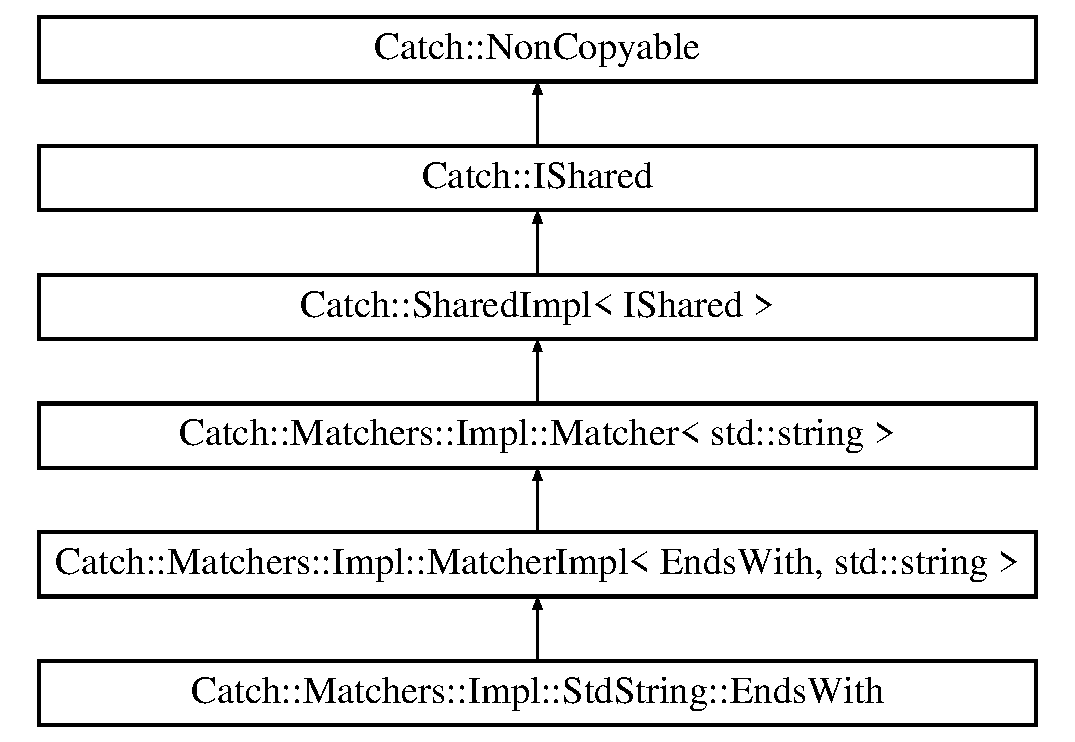
\includegraphics[height=6.000000cm]{structCatch_1_1Matchers_1_1Impl_1_1StdString_1_1EndsWith}
\end{center}
\end{figure}
\subsection*{Public Member Functions}
\begin{DoxyCompactItemize}
\item 
{\bfseries Ends\+With} (std\+::string const \&substr, Case\+Sensitive\+::\+Choice case\+Sensitivity=Case\+Sensitive\+::\+Yes)\hypertarget{structCatch_1_1Matchers_1_1Impl_1_1StdString_1_1EndsWith_ae90c02ff06c9dd5e62218b2b521e8cab}{}\label{structCatch_1_1Matchers_1_1Impl_1_1StdString_1_1EndsWith_ae90c02ff06c9dd5e62218b2b521e8cab}

\item 
{\bfseries Ends\+With} (\hyperlink{structCatch_1_1Matchers_1_1Impl_1_1StdString_1_1EndsWith}{Ends\+With} const \&other)\hypertarget{structCatch_1_1Matchers_1_1Impl_1_1StdString_1_1EndsWith_a9321aac07fb17613a7993e99003b3be2}{}\label{structCatch_1_1Matchers_1_1Impl_1_1StdString_1_1EndsWith_a9321aac07fb17613a7993e99003b3be2}

\item 
virtual bool {\bfseries match} (std\+::string const \&expr) const \hypertarget{structCatch_1_1Matchers_1_1Impl_1_1StdString_1_1EndsWith_ad0e03d7f54ffa5859f84faebccf11e76}{}\label{structCatch_1_1Matchers_1_1Impl_1_1StdString_1_1EndsWith_ad0e03d7f54ffa5859f84faebccf11e76}

\item 
virtual std\+::string {\bfseries to\+String} () const \hypertarget{structCatch_1_1Matchers_1_1Impl_1_1StdString_1_1EndsWith_a54715c94c215a1fc5fb6336acf52eb06}{}\label{structCatch_1_1Matchers_1_1Impl_1_1StdString_1_1EndsWith_a54715c94c215a1fc5fb6336acf52eb06}

\end{DoxyCompactItemize}
\subsection*{Public Attributes}
\begin{DoxyCompactItemize}
\item 
\hyperlink{structCatch_1_1Matchers_1_1Impl_1_1StdString_1_1CasedString}{Cased\+String} {\bfseries m\+\_\+data}\hypertarget{structCatch_1_1Matchers_1_1Impl_1_1StdString_1_1EndsWith_a344d8433f3ba3e0de301ab16ed6dd746}{}\label{structCatch_1_1Matchers_1_1Impl_1_1StdString_1_1EndsWith_a344d8433f3ba3e0de301ab16ed6dd746}

\end{DoxyCompactItemize}
\subsection*{Additional Inherited Members}


The documentation for this struct was generated from the following file\+:\begin{DoxyCompactItemize}
\item 
catch.\+hpp\end{DoxyCompactItemize}

\hypertarget{structCatch_1_1Matchers_1_1Impl_1_1StdString_1_1Equals}{}\section{Catch\+:\+:Matchers\+:\+:Impl\+:\+:Std\+String\+:\+:Equals Struct Reference}
\label{structCatch_1_1Matchers_1_1Impl_1_1StdString_1_1Equals}\index{Catch\+::\+Matchers\+::\+Impl\+::\+Std\+String\+::\+Equals@{Catch\+::\+Matchers\+::\+Impl\+::\+Std\+String\+::\+Equals}}
Inheritance diagram for Catch\+:\+:Matchers\+:\+:Impl\+:\+:Std\+String\+:\+:Equals\+:\begin{figure}[H]
\begin{center}
\leavevmode
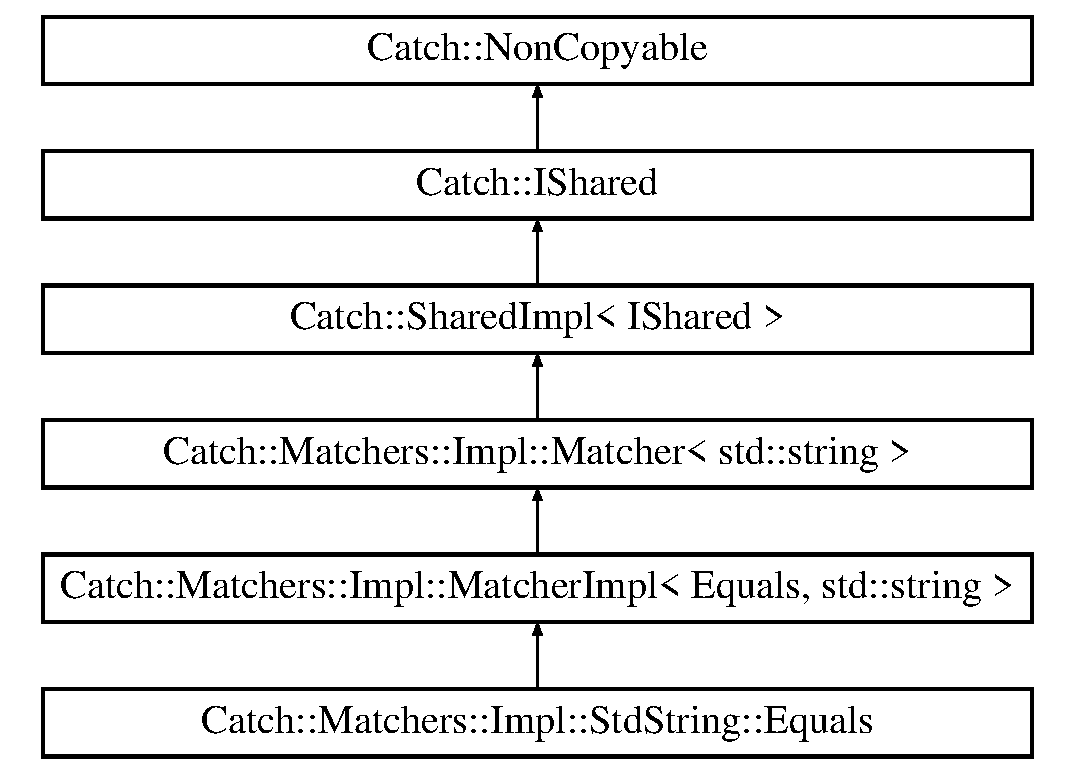
\includegraphics[height=6.000000cm]{structCatch_1_1Matchers_1_1Impl_1_1StdString_1_1Equals}
\end{center}
\end{figure}
\subsection*{Public Member Functions}
\begin{DoxyCompactItemize}
\item 
{\bfseries Equals} (std\+::string const \&str, Case\+Sensitive\+::\+Choice case\+Sensitivity=Case\+Sensitive\+::\+Yes)\hypertarget{structCatch_1_1Matchers_1_1Impl_1_1StdString_1_1Equals_a5921d5ed75320fb64a678e3f1292a464}{}\label{structCatch_1_1Matchers_1_1Impl_1_1StdString_1_1Equals_a5921d5ed75320fb64a678e3f1292a464}

\item 
{\bfseries Equals} (\hyperlink{structCatch_1_1Matchers_1_1Impl_1_1StdString_1_1Equals}{Equals} const \&other)\hypertarget{structCatch_1_1Matchers_1_1Impl_1_1StdString_1_1Equals_acaa97de06aedf363ae803d65a975f5e4}{}\label{structCatch_1_1Matchers_1_1Impl_1_1StdString_1_1Equals_acaa97de06aedf363ae803d65a975f5e4}

\item 
virtual bool {\bfseries match} (std\+::string const \&expr) const \hypertarget{structCatch_1_1Matchers_1_1Impl_1_1StdString_1_1Equals_a00c8259a76c24da669e116662ededc70}{}\label{structCatch_1_1Matchers_1_1Impl_1_1StdString_1_1Equals_a00c8259a76c24da669e116662ededc70}

\item 
virtual std\+::string {\bfseries to\+String} () const \hypertarget{structCatch_1_1Matchers_1_1Impl_1_1StdString_1_1Equals_a7a09449ff2f858981caf3b1f6c36d270}{}\label{structCatch_1_1Matchers_1_1Impl_1_1StdString_1_1Equals_a7a09449ff2f858981caf3b1f6c36d270}

\end{DoxyCompactItemize}
\subsection*{Public Attributes}
\begin{DoxyCompactItemize}
\item 
\hyperlink{structCatch_1_1Matchers_1_1Impl_1_1StdString_1_1CasedString}{Cased\+String} {\bfseries m\+\_\+data}\hypertarget{structCatch_1_1Matchers_1_1Impl_1_1StdString_1_1Equals_ae09964b7ba291ce574b514a2ee3eddb0}{}\label{structCatch_1_1Matchers_1_1Impl_1_1StdString_1_1Equals_ae09964b7ba291ce574b514a2ee3eddb0}

\end{DoxyCompactItemize}
\subsection*{Additional Inherited Members}


The documentation for this struct was generated from the following file\+:\begin{DoxyCompactItemize}
\item 
catch.\+hpp\end{DoxyCompactItemize}

\hypertarget{classCatch_1_1Internal_1_1Evaluator}{}\section{Catch\+:\+:Internal\+:\+:Evaluator$<$ T1, T2, Op $>$ Class Template Reference}
\label{classCatch_1_1Internal_1_1Evaluator}\index{Catch\+::\+Internal\+::\+Evaluator$<$ T1, T2, Op $>$@{Catch\+::\+Internal\+::\+Evaluator$<$ T1, T2, Op $>$}}


The documentation for this class was generated from the following file\+:\begin{DoxyCompactItemize}
\item 
catch.\+hpp\end{DoxyCompactItemize}

\hypertarget{structCatch_1_1Internal_1_1Evaluator_3_01T1_00_01T2_00_01IsEqualTo_01_4}{}\section{Catch\+:\+:Internal\+:\+:Evaluator$<$ T1, T2, Is\+Equal\+To $>$ Struct Template Reference}
\label{structCatch_1_1Internal_1_1Evaluator_3_01T1_00_01T2_00_01IsEqualTo_01_4}\index{Catch\+::\+Internal\+::\+Evaluator$<$ T1, T2, Is\+Equal\+To $>$@{Catch\+::\+Internal\+::\+Evaluator$<$ T1, T2, Is\+Equal\+To $>$}}
\subsection*{Static Public Member Functions}
\begin{DoxyCompactItemize}
\item 
static bool {\bfseries evaluate} (T1 const \&lhs, T2 const \&rhs)\hypertarget{structCatch_1_1Internal_1_1Evaluator_3_01T1_00_01T2_00_01IsEqualTo_01_4_a166b2b7849247397e63fb2940481b217}{}\label{structCatch_1_1Internal_1_1Evaluator_3_01T1_00_01T2_00_01IsEqualTo_01_4_a166b2b7849247397e63fb2940481b217}

\end{DoxyCompactItemize}


The documentation for this struct was generated from the following file\+:\begin{DoxyCompactItemize}
\item 
catch.\+hpp\end{DoxyCompactItemize}

\hypertarget{structCatch_1_1Internal_1_1Evaluator_3_01T1_00_01T2_00_01IsGreaterThan_01_4}{}\section{Catch\+:\+:Internal\+:\+:Evaluator$<$ T1, T2, Is\+Greater\+Than $>$ Struct Template Reference}
\label{structCatch_1_1Internal_1_1Evaluator_3_01T1_00_01T2_00_01IsGreaterThan_01_4}\index{Catch\+::\+Internal\+::\+Evaluator$<$ T1, T2, Is\+Greater\+Than $>$@{Catch\+::\+Internal\+::\+Evaluator$<$ T1, T2, Is\+Greater\+Than $>$}}
\subsection*{Static Public Member Functions}
\begin{DoxyCompactItemize}
\item 
static bool {\bfseries evaluate} (T1 const \&lhs, T2 const \&rhs)\hypertarget{structCatch_1_1Internal_1_1Evaluator_3_01T1_00_01T2_00_01IsGreaterThan_01_4_a55745f74f09ac5c61bd3d592ca5560af}{}\label{structCatch_1_1Internal_1_1Evaluator_3_01T1_00_01T2_00_01IsGreaterThan_01_4_a55745f74f09ac5c61bd3d592ca5560af}

\end{DoxyCompactItemize}


The documentation for this struct was generated from the following file\+:\begin{DoxyCompactItemize}
\item 
catch.\+hpp\end{DoxyCompactItemize}

\hypertarget{structCatch_1_1Internal_1_1Evaluator_3_01T1_00_01T2_00_01IsGreaterThanOrEqualTo_01_4}{}\section{Catch\+:\+:Internal\+:\+:Evaluator$<$ T1, T2, Is\+Greater\+Than\+Or\+Equal\+To $>$ Struct Template Reference}
\label{structCatch_1_1Internal_1_1Evaluator_3_01T1_00_01T2_00_01IsGreaterThanOrEqualTo_01_4}\index{Catch\+::\+Internal\+::\+Evaluator$<$ T1, T2, Is\+Greater\+Than\+Or\+Equal\+To $>$@{Catch\+::\+Internal\+::\+Evaluator$<$ T1, T2, Is\+Greater\+Than\+Or\+Equal\+To $>$}}
\subsection*{Static Public Member Functions}
\begin{DoxyCompactItemize}
\item 
static bool {\bfseries evaluate} (T1 const \&lhs, T2 const \&rhs)\hypertarget{structCatch_1_1Internal_1_1Evaluator_3_01T1_00_01T2_00_01IsGreaterThanOrEqualTo_01_4_a5ba107c6da4292b6492a0e5e906f9484}{}\label{structCatch_1_1Internal_1_1Evaluator_3_01T1_00_01T2_00_01IsGreaterThanOrEqualTo_01_4_a5ba107c6da4292b6492a0e5e906f9484}

\end{DoxyCompactItemize}


The documentation for this struct was generated from the following file\+:\begin{DoxyCompactItemize}
\item 
catch.\+hpp\end{DoxyCompactItemize}

\hypertarget{structCatch_1_1Internal_1_1Evaluator_3_01T1_00_01T2_00_01IsLessThan_01_4}{}\section{Catch\+:\+:Internal\+:\+:Evaluator$<$ T1, T2, Is\+Less\+Than $>$ Struct Template Reference}
\label{structCatch_1_1Internal_1_1Evaluator_3_01T1_00_01T2_00_01IsLessThan_01_4}\index{Catch\+::\+Internal\+::\+Evaluator$<$ T1, T2, Is\+Less\+Than $>$@{Catch\+::\+Internal\+::\+Evaluator$<$ T1, T2, Is\+Less\+Than $>$}}
\subsection*{Static Public Member Functions}
\begin{DoxyCompactItemize}
\item 
static bool {\bfseries evaluate} (T1 const \&lhs, T2 const \&rhs)\hypertarget{structCatch_1_1Internal_1_1Evaluator_3_01T1_00_01T2_00_01IsLessThan_01_4_a75b2bcf80ce6f90218c145e2c3293d75}{}\label{structCatch_1_1Internal_1_1Evaluator_3_01T1_00_01T2_00_01IsLessThan_01_4_a75b2bcf80ce6f90218c145e2c3293d75}

\end{DoxyCompactItemize}


The documentation for this struct was generated from the following file\+:\begin{DoxyCompactItemize}
\item 
catch.\+hpp\end{DoxyCompactItemize}

\hypertarget{structCatch_1_1Internal_1_1Evaluator_3_01T1_00_01T2_00_01IsLessThanOrEqualTo_01_4}{}\section{Catch\+:\+:Internal\+:\+:Evaluator$<$ T1, T2, Is\+Less\+Than\+Or\+Equal\+To $>$ Struct Template Reference}
\label{structCatch_1_1Internal_1_1Evaluator_3_01T1_00_01T2_00_01IsLessThanOrEqualTo_01_4}\index{Catch\+::\+Internal\+::\+Evaluator$<$ T1, T2, Is\+Less\+Than\+Or\+Equal\+To $>$@{Catch\+::\+Internal\+::\+Evaluator$<$ T1, T2, Is\+Less\+Than\+Or\+Equal\+To $>$}}
\subsection*{Static Public Member Functions}
\begin{DoxyCompactItemize}
\item 
static bool {\bfseries evaluate} (T1 const \&lhs, T2 const \&rhs)\hypertarget{structCatch_1_1Internal_1_1Evaluator_3_01T1_00_01T2_00_01IsLessThanOrEqualTo_01_4_adf269a597e4d82d69f29bcb516297b9b}{}\label{structCatch_1_1Internal_1_1Evaluator_3_01T1_00_01T2_00_01IsLessThanOrEqualTo_01_4_adf269a597e4d82d69f29bcb516297b9b}

\end{DoxyCompactItemize}


The documentation for this struct was generated from the following file\+:\begin{DoxyCompactItemize}
\item 
catch.\+hpp\end{DoxyCompactItemize}

\hypertarget{structCatch_1_1Internal_1_1Evaluator_3_01T1_00_01T2_00_01IsNotEqualTo_01_4}{}\section{Catch\+:\+:Internal\+:\+:Evaluator$<$ T1, T2, Is\+Not\+Equal\+To $>$ Struct Template Reference}
\label{structCatch_1_1Internal_1_1Evaluator_3_01T1_00_01T2_00_01IsNotEqualTo_01_4}\index{Catch\+::\+Internal\+::\+Evaluator$<$ T1, T2, Is\+Not\+Equal\+To $>$@{Catch\+::\+Internal\+::\+Evaluator$<$ T1, T2, Is\+Not\+Equal\+To $>$}}
\subsection*{Static Public Member Functions}
\begin{DoxyCompactItemize}
\item 
static bool {\bfseries evaluate} (T1 const \&lhs, T2 const \&rhs)\hypertarget{structCatch_1_1Internal_1_1Evaluator_3_01T1_00_01T2_00_01IsNotEqualTo_01_4_a956a12d0f4a7dceb5a1ce914421ff945}{}\label{structCatch_1_1Internal_1_1Evaluator_3_01T1_00_01T2_00_01IsNotEqualTo_01_4_a956a12d0f4a7dceb5a1ce914421ff945}

\end{DoxyCompactItemize}


The documentation for this struct was generated from the following file\+:\begin{DoxyCompactItemize}
\item 
catch.\+hpp\end{DoxyCompactItemize}

\hypertarget{classCatch_1_1ExceptionTranslatorRegistrar}{}\section{Catch\+:\+:Exception\+Translator\+Registrar Class Reference}
\label{classCatch_1_1ExceptionTranslatorRegistrar}\index{Catch\+::\+Exception\+Translator\+Registrar@{Catch\+::\+Exception\+Translator\+Registrar}}
\subsection*{Public Member Functions}
\begin{DoxyCompactItemize}
\item 
{\footnotesize template$<$typename T $>$ }\\{\bfseries Exception\+Translator\+Registrar} (std\+::string($\ast$translate\+Function)(T \&))\hypertarget{classCatch_1_1ExceptionTranslatorRegistrar_aa73229de911f26b1df6c6c87c4d9e04e}{}\label{classCatch_1_1ExceptionTranslatorRegistrar_aa73229de911f26b1df6c6c87c4d9e04e}

\end{DoxyCompactItemize}


The documentation for this class was generated from the following file\+:\begin{DoxyCompactItemize}
\item 
catch.\+hpp\end{DoxyCompactItemize}

\hypertarget{classCatch_1_1ExpressionLhs}{}\section{Catch\+:\+:Expression\+Lhs$<$ T $>$ Class Template Reference}
\label{classCatch_1_1ExpressionLhs}\index{Catch\+::\+Expression\+Lhs$<$ T $>$@{Catch\+::\+Expression\+Lhs$<$ T $>$}}
\subsection*{Public Member Functions}
\begin{DoxyCompactItemize}
\item 
{\bfseries Expression\+Lhs} (\hyperlink{classCatch_1_1ResultBuilder}{Result\+Builder} \&rb, T lhs)\hypertarget{classCatch_1_1ExpressionLhs_aa829588def6146a94fb75de9c4cc482a}{}\label{classCatch_1_1ExpressionLhs_aa829588def6146a94fb75de9c4cc482a}

\item 
{\footnotesize template$<$typename RhsT $>$ }\\\hyperlink{classCatch_1_1ResultBuilder}{Result\+Builder} \& {\bfseries operator==} (RhsT const \&rhs)\hypertarget{classCatch_1_1ExpressionLhs_a2f7ad442c3e5e5764eee736345c40301}{}\label{classCatch_1_1ExpressionLhs_a2f7ad442c3e5e5764eee736345c40301}

\item 
{\footnotesize template$<$typename RhsT $>$ }\\\hyperlink{classCatch_1_1ResultBuilder}{Result\+Builder} \& {\bfseries operator!=} (RhsT const \&rhs)\hypertarget{classCatch_1_1ExpressionLhs_a44df9974cf20fcfda4e5b6b3c01d5f93}{}\label{classCatch_1_1ExpressionLhs_a44df9974cf20fcfda4e5b6b3c01d5f93}

\item 
{\footnotesize template$<$typename RhsT $>$ }\\\hyperlink{classCatch_1_1ResultBuilder}{Result\+Builder} \& {\bfseries operator$<$} (RhsT const \&rhs)\hypertarget{classCatch_1_1ExpressionLhs_a48428d358ddc89729e2e3407f4024dac}{}\label{classCatch_1_1ExpressionLhs_a48428d358ddc89729e2e3407f4024dac}

\item 
{\footnotesize template$<$typename RhsT $>$ }\\\hyperlink{classCatch_1_1ResultBuilder}{Result\+Builder} \& {\bfseries operator$>$} (RhsT const \&rhs)\hypertarget{classCatch_1_1ExpressionLhs_ad3602a7ad945c751004065b1007dc183}{}\label{classCatch_1_1ExpressionLhs_ad3602a7ad945c751004065b1007dc183}

\item 
{\footnotesize template$<$typename RhsT $>$ }\\\hyperlink{classCatch_1_1ResultBuilder}{Result\+Builder} \& {\bfseries operator$<$=} (RhsT const \&rhs)\hypertarget{classCatch_1_1ExpressionLhs_afd188990e8a14b49c308ce7a79056846}{}\label{classCatch_1_1ExpressionLhs_afd188990e8a14b49c308ce7a79056846}

\item 
{\footnotesize template$<$typename RhsT $>$ }\\\hyperlink{classCatch_1_1ResultBuilder}{Result\+Builder} \& {\bfseries operator$>$=} (RhsT const \&rhs)\hypertarget{classCatch_1_1ExpressionLhs_a21d30d6026ff2b1f86ddbd6b0a90d036}{}\label{classCatch_1_1ExpressionLhs_a21d30d6026ff2b1f86ddbd6b0a90d036}

\item 
\hyperlink{classCatch_1_1ResultBuilder}{Result\+Builder} \& {\bfseries operator==} (bool rhs)\hypertarget{classCatch_1_1ExpressionLhs_a6001030bcfbabc3981013ddffb3e3bb6}{}\label{classCatch_1_1ExpressionLhs_a6001030bcfbabc3981013ddffb3e3bb6}

\item 
\hyperlink{classCatch_1_1ResultBuilder}{Result\+Builder} \& {\bfseries operator!=} (bool rhs)\hypertarget{classCatch_1_1ExpressionLhs_a71e48da9a894962e8b32a8af5359a4df}{}\label{classCatch_1_1ExpressionLhs_a71e48da9a894962e8b32a8af5359a4df}

\item 
void {\bfseries end\+Expression} ()\hypertarget{classCatch_1_1ExpressionLhs_a13d2551a927790284fb5ddf1ee2c9079}{}\label{classCatch_1_1ExpressionLhs_a13d2551a927790284fb5ddf1ee2c9079}

\item 
{\footnotesize template$<$typename RhsT $>$ }\\S\+T\+A\+T\+I\+C\+\_\+\+A\+S\+S\+E\+R\+T\+\_\+\+Expression\+\_\+\+Too\+\_\+\+Complex\+\_\+\+Please\+\_\+\+Rewrite\+\_\+\+As\+\_\+\+Binary\+\_\+\+Comparison \& {\bfseries operator+} (RhsT const \&)\hypertarget{classCatch_1_1ExpressionLhs_a29ffb8417e977f0a98c0eb537a7ca5af}{}\label{classCatch_1_1ExpressionLhs_a29ffb8417e977f0a98c0eb537a7ca5af}

\item 
{\footnotesize template$<$typename RhsT $>$ }\\S\+T\+A\+T\+I\+C\+\_\+\+A\+S\+S\+E\+R\+T\+\_\+\+Expression\+\_\+\+Too\+\_\+\+Complex\+\_\+\+Please\+\_\+\+Rewrite\+\_\+\+As\+\_\+\+Binary\+\_\+\+Comparison \& {\bfseries operator-\/} (RhsT const \&)\hypertarget{classCatch_1_1ExpressionLhs_a19ef0a33442bb18efef1ec65102151d1}{}\label{classCatch_1_1ExpressionLhs_a19ef0a33442bb18efef1ec65102151d1}

\item 
{\footnotesize template$<$typename RhsT $>$ }\\S\+T\+A\+T\+I\+C\+\_\+\+A\+S\+S\+E\+R\+T\+\_\+\+Expression\+\_\+\+Too\+\_\+\+Complex\+\_\+\+Please\+\_\+\+Rewrite\+\_\+\+As\+\_\+\+Binary\+\_\+\+Comparison \& {\bfseries operator/} (RhsT const \&)\hypertarget{classCatch_1_1ExpressionLhs_a37d50565046ac9b1c9159a7c0cf88a1e}{}\label{classCatch_1_1ExpressionLhs_a37d50565046ac9b1c9159a7c0cf88a1e}

\item 
{\footnotesize template$<$typename RhsT $>$ }\\S\+T\+A\+T\+I\+C\+\_\+\+A\+S\+S\+E\+R\+T\+\_\+\+Expression\+\_\+\+Too\+\_\+\+Complex\+\_\+\+Please\+\_\+\+Rewrite\+\_\+\+As\+\_\+\+Binary\+\_\+\+Comparison \& {\bfseries operator$\ast$} (RhsT const \&)\hypertarget{classCatch_1_1ExpressionLhs_a9a94294c22449f62087862ef911e6291}{}\label{classCatch_1_1ExpressionLhs_a9a94294c22449f62087862ef911e6291}

\item 
{\footnotesize template$<$typename RhsT $>$ }\\S\+T\+A\+T\+I\+C\+\_\+\+A\+S\+S\+E\+R\+T\+\_\+\+Expression\+\_\+\+Too\+\_\+\+Complex\+\_\+\+Please\+\_\+\+Rewrite\+\_\+\+As\+\_\+\+Binary\+\_\+\+Comparison \& {\bfseries operator\&\&} (RhsT const \&)\hypertarget{classCatch_1_1ExpressionLhs_a7f022056ef4f25e716ab85846be6229f}{}\label{classCatch_1_1ExpressionLhs_a7f022056ef4f25e716ab85846be6229f}

\item 
{\footnotesize template$<$typename RhsT $>$ }\\S\+T\+A\+T\+I\+C\+\_\+\+A\+S\+S\+E\+R\+T\+\_\+\+Expression\+\_\+\+Too\+\_\+\+Complex\+\_\+\+Please\+\_\+\+Rewrite\+\_\+\+As\+\_\+\+Binary\+\_\+\+Comparison \& {\bfseries operator$\vert$$\vert$} (RhsT const \&)\hypertarget{classCatch_1_1ExpressionLhs_a6932b72da79d6c6b03d867772ceac61b}{}\label{classCatch_1_1ExpressionLhs_a6932b72da79d6c6b03d867772ceac61b}

\end{DoxyCompactItemize}


The documentation for this class was generated from the following file\+:\begin{DoxyCompactItemize}
\item 
catch.\+hpp\end{DoxyCompactItemize}

\hypertarget{structCatch_1_1Detail_1_1FalseType}{}\section{Catch\+:\+:Detail\+:\+:False\+Type Struct Reference}
\label{structCatch_1_1Detail_1_1FalseType}\index{Catch\+::\+Detail\+::\+False\+Type@{Catch\+::\+Detail\+::\+False\+Type}}
\subsection*{Public Attributes}
\begin{DoxyCompactItemize}
\item 
char {\bfseries sizer} \mbox{[}2\mbox{]}\hypertarget{structCatch_1_1Detail_1_1FalseType_abc1a730e197d6f7750ae8aaf47b63477}{}\label{structCatch_1_1Detail_1_1FalseType_abc1a730e197d6f7750ae8aaf47b63477}

\end{DoxyCompactItemize}


The documentation for this struct was generated from the following file\+:\begin{DoxyCompactItemize}
\item 
catch.\+hpp\end{DoxyCompactItemize}

\hypertarget{structCatch_1_1IContext}{}\section{Catch\+:\+:I\+Context Struct Reference}
\label{structCatch_1_1IContext}\index{Catch\+::\+I\+Context@{Catch\+::\+I\+Context}}
Inheritance diagram for Catch\+:\+:I\+Context\+:\begin{figure}[H]
\begin{center}
\leavevmode
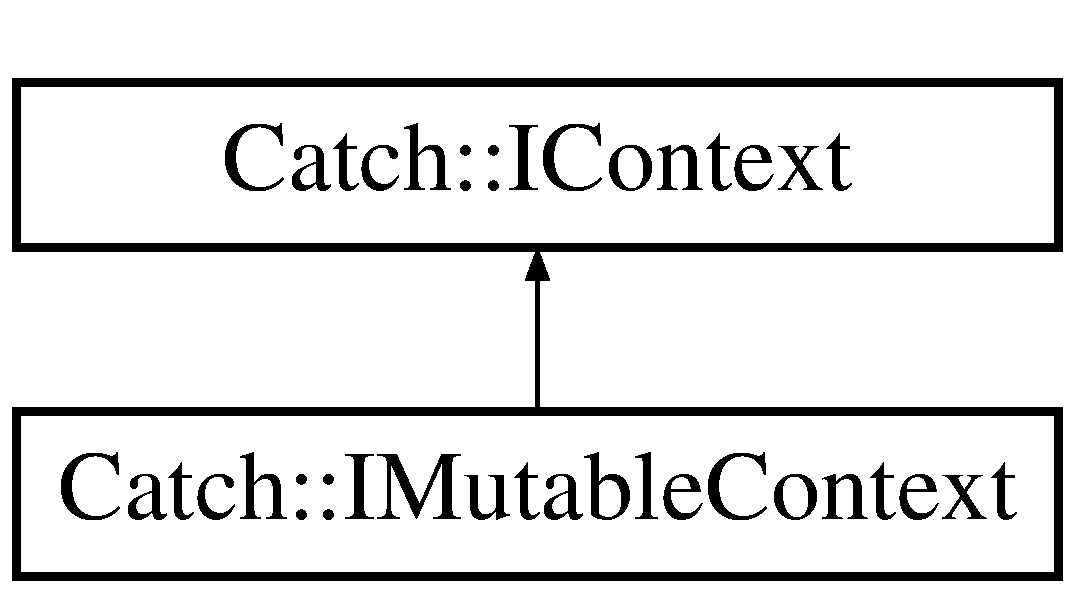
\includegraphics[height=2.000000cm]{structCatch_1_1IContext}
\end{center}
\end{figure}
\subsection*{Public Member Functions}
\begin{DoxyCompactItemize}
\item 
virtual \hyperlink{structCatch_1_1IResultCapture}{I\+Result\+Capture} $\ast$ {\bfseries get\+Result\+Capture} ()=0\hypertarget{structCatch_1_1IContext_a684e4ae71d1fdf3060c352ecde1d122f}{}\label{structCatch_1_1IContext_a684e4ae71d1fdf3060c352ecde1d122f}

\item 
virtual \hyperlink{structCatch_1_1IRunner}{I\+Runner} $\ast$ {\bfseries get\+Runner} ()=0\hypertarget{structCatch_1_1IContext_af088415dde18d039ed5a2f95b02767c6}{}\label{structCatch_1_1IContext_af088415dde18d039ed5a2f95b02767c6}

\item 
virtual size\+\_\+t {\bfseries get\+Generator\+Index} (std\+::string const \&file\+Info, size\+\_\+t total\+Size)=0\hypertarget{structCatch_1_1IContext_a43e07088db43299ba129fbe6d3106e95}{}\label{structCatch_1_1IContext_a43e07088db43299ba129fbe6d3106e95}

\item 
virtual bool {\bfseries advance\+Generators\+For\+Current\+Test} ()=0\hypertarget{structCatch_1_1IContext_a806f7c4ed24d51adae90418e661b24b7}{}\label{structCatch_1_1IContext_a806f7c4ed24d51adae90418e661b24b7}

\item 
virtual \hyperlink{classCatch_1_1Ptr}{Ptr}$<$ I\+Config const  $>$ {\bfseries get\+Config} () const  =0\hypertarget{structCatch_1_1IContext_a9b6759547b9af1e77b6bc9f0dd596ac2}{}\label{structCatch_1_1IContext_a9b6759547b9af1e77b6bc9f0dd596ac2}

\end{DoxyCompactItemize}


The documentation for this struct was generated from the following file\+:\begin{DoxyCompactItemize}
\item 
catch.\+hpp\end{DoxyCompactItemize}

\hypertarget{structCatch_1_1IExceptionTranslator}{}\section{Catch\+:\+:I\+Exception\+Translator Struct Reference}
\label{structCatch_1_1IExceptionTranslator}\index{Catch\+::\+I\+Exception\+Translator@{Catch\+::\+I\+Exception\+Translator}}
\subsection*{Public Member Functions}
\begin{DoxyCompactItemize}
\item 
virtual std\+::string {\bfseries translate} (Exception\+Translators\+::const\+\_\+iterator it, Exception\+Translators\+::const\+\_\+iterator it\+End) const  =0\hypertarget{structCatch_1_1IExceptionTranslator_aab7251b547758dadfe2d87b367a7eddd}{}\label{structCatch_1_1IExceptionTranslator_aab7251b547758dadfe2d87b367a7eddd}

\end{DoxyCompactItemize}


The documentation for this struct was generated from the following file\+:\begin{DoxyCompactItemize}
\item 
catch.\+hpp\end{DoxyCompactItemize}

\hypertarget{structCatch_1_1IExceptionTranslatorRegistry}{}\section{Catch\+:\+:I\+Exception\+Translator\+Registry Struct Reference}
\label{structCatch_1_1IExceptionTranslatorRegistry}\index{Catch\+::\+I\+Exception\+Translator\+Registry@{Catch\+::\+I\+Exception\+Translator\+Registry}}
\subsection*{Public Member Functions}
\begin{DoxyCompactItemize}
\item 
virtual std\+::string {\bfseries translate\+Active\+Exception} () const  =0\hypertarget{structCatch_1_1IExceptionTranslatorRegistry_ad51c26856187bb69da6b43dbcd59cf18}{}\label{structCatch_1_1IExceptionTranslatorRegistry_ad51c26856187bb69da6b43dbcd59cf18}

\end{DoxyCompactItemize}


The documentation for this struct was generated from the following file\+:\begin{DoxyCompactItemize}
\item 
catch.\+hpp\end{DoxyCompactItemize}

\hypertarget{structCatch_1_1IGenerator}{}\section{Catch\+:\+:I\+Generator$<$ T $>$ Struct Template Reference}
\label{structCatch_1_1IGenerator}\index{Catch\+::\+I\+Generator$<$ T $>$@{Catch\+::\+I\+Generator$<$ T $>$}}
Inheritance diagram for Catch\+:\+:I\+Generator$<$ T $>$\+:\begin{figure}[H]
\begin{center}
\leavevmode
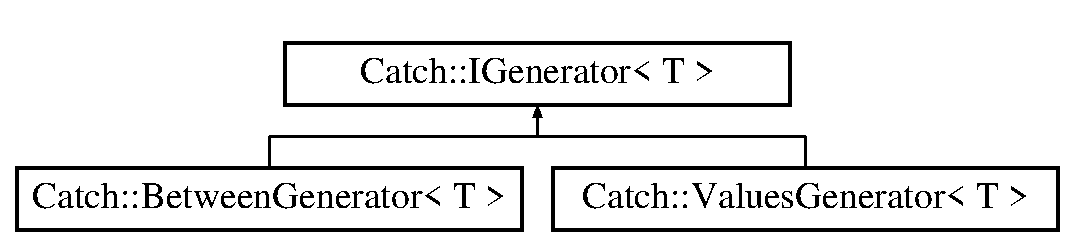
\includegraphics[height=2.000000cm]{structCatch_1_1IGenerator}
\end{center}
\end{figure}
\subsection*{Public Member Functions}
\begin{DoxyCompactItemize}
\item 
virtual T {\bfseries get\+Value} (std\+::size\+\_\+t index) const  =0\hypertarget{structCatch_1_1IGenerator_a242bb447d6a37784215be6df7d44bb6a}{}\label{structCatch_1_1IGenerator_a242bb447d6a37784215be6df7d44bb6a}

\item 
virtual std\+::size\+\_\+t {\bfseries size} () const  =0\hypertarget{structCatch_1_1IGenerator_a9a03cf8579a60da0714fda6e5bd0af04}{}\label{structCatch_1_1IGenerator_a9a03cf8579a60da0714fda6e5bd0af04}

\end{DoxyCompactItemize}


The documentation for this struct was generated from the following file\+:\begin{DoxyCompactItemize}
\item 
catch.\+hpp\end{DoxyCompactItemize}

\hypertarget{structCatch_1_1IGeneratorInfo}{}\section{Catch\+:\+:I\+Generator\+Info Struct Reference}
\label{structCatch_1_1IGeneratorInfo}\index{Catch\+::\+I\+Generator\+Info@{Catch\+::\+I\+Generator\+Info}}
\subsection*{Public Member Functions}
\begin{DoxyCompactItemize}
\item 
virtual bool {\bfseries move\+Next} ()=0\hypertarget{structCatch_1_1IGeneratorInfo_a2b86711ca7009903edfe27ed62b515ef}{}\label{structCatch_1_1IGeneratorInfo_a2b86711ca7009903edfe27ed62b515ef}

\item 
virtual std\+::size\+\_\+t {\bfseries get\+Current\+Index} () const  =0\hypertarget{structCatch_1_1IGeneratorInfo_adc7a8e218463e9e7ce8732ad1f588914}{}\label{structCatch_1_1IGeneratorInfo_adc7a8e218463e9e7ce8732ad1f588914}

\end{DoxyCompactItemize}


The documentation for this struct was generated from the following file\+:\begin{DoxyCompactItemize}
\item 
catch.\+hpp\end{DoxyCompactItemize}

\hypertarget{structCatch_1_1IGeneratorsForTest}{}\section{Catch\+:\+:I\+Generators\+For\+Test Struct Reference}
\label{structCatch_1_1IGeneratorsForTest}\index{Catch\+::\+I\+Generators\+For\+Test@{Catch\+::\+I\+Generators\+For\+Test}}
\subsection*{Public Member Functions}
\begin{DoxyCompactItemize}
\item 
virtual \hyperlink{structCatch_1_1IGeneratorInfo}{I\+Generator\+Info} \& {\bfseries get\+Generator\+Info} (std\+::string const \&file\+Info, std\+::size\+\_\+t size)=0\hypertarget{structCatch_1_1IGeneratorsForTest_a180d84e858840188e4c3788e47eefdb0}{}\label{structCatch_1_1IGeneratorsForTest_a180d84e858840188e4c3788e47eefdb0}

\item 
virtual bool {\bfseries move\+Next} ()=0\hypertarget{structCatch_1_1IGeneratorsForTest_adab31832d529fc584fd63164e0a1c8ad}{}\label{structCatch_1_1IGeneratorsForTest_adab31832d529fc584fd63164e0a1c8ad}

\end{DoxyCompactItemize}


The documentation for this struct was generated from the following file\+:\begin{DoxyCompactItemize}
\item 
catch.\+hpp\end{DoxyCompactItemize}

\hypertarget{structCatch_1_1IMutableContext}{}\section{Catch\+:\+:I\+Mutable\+Context Struct Reference}
\label{structCatch_1_1IMutableContext}\index{Catch\+::\+I\+Mutable\+Context@{Catch\+::\+I\+Mutable\+Context}}
Inheritance diagram for Catch\+:\+:I\+Mutable\+Context\+:\begin{figure}[H]
\begin{center}
\leavevmode
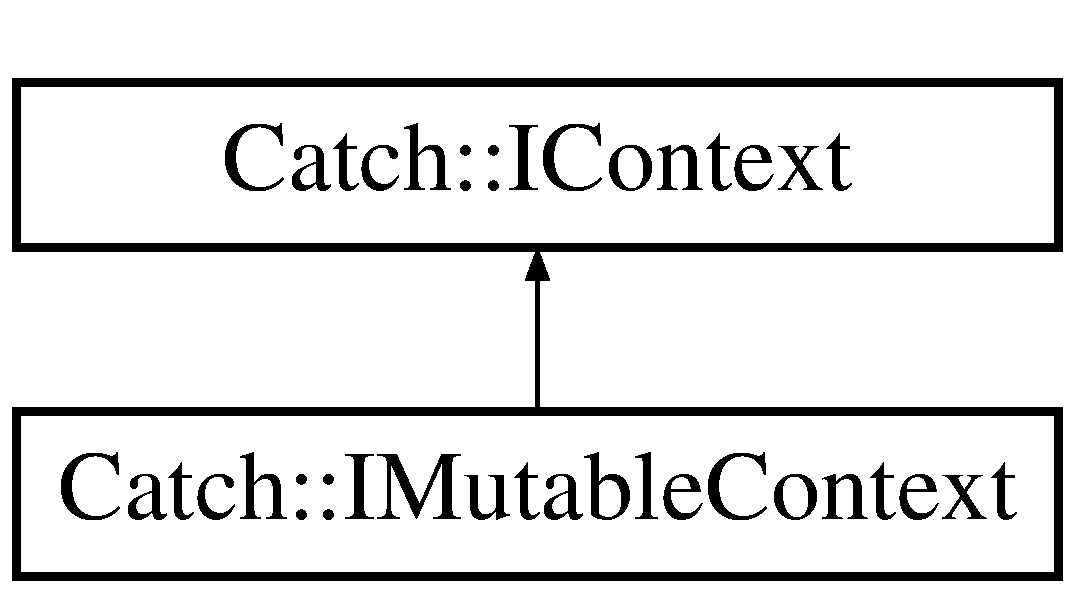
\includegraphics[height=2.000000cm]{structCatch_1_1IMutableContext}
\end{center}
\end{figure}
\subsection*{Public Member Functions}
\begin{DoxyCompactItemize}
\item 
virtual void {\bfseries set\+Result\+Capture} (\hyperlink{structCatch_1_1IResultCapture}{I\+Result\+Capture} $\ast$result\+Capture)=0\hypertarget{structCatch_1_1IMutableContext_a4a80afd0525b7def21bee8d9b48f2d39}{}\label{structCatch_1_1IMutableContext_a4a80afd0525b7def21bee8d9b48f2d39}

\item 
virtual void {\bfseries set\+Runner} (\hyperlink{structCatch_1_1IRunner}{I\+Runner} $\ast$runner)=0\hypertarget{structCatch_1_1IMutableContext_af2e53b1dea4527a2587cff266a730f6e}{}\label{structCatch_1_1IMutableContext_af2e53b1dea4527a2587cff266a730f6e}

\item 
virtual void {\bfseries set\+Config} (\hyperlink{classCatch_1_1Ptr}{Ptr}$<$ I\+Config const  $>$ const \&config)=0\hypertarget{structCatch_1_1IMutableContext_a04ae4f4219a481a7bf658d9fd445bc1d}{}\label{structCatch_1_1IMutableContext_a04ae4f4219a481a7bf658d9fd445bc1d}

\end{DoxyCompactItemize}


The documentation for this struct was generated from the following file\+:\begin{DoxyCompactItemize}
\item 
catch.\+hpp\end{DoxyCompactItemize}

\hypertarget{structCatch_1_1IMutableRegistryHub}{}\section{Catch\+:\+:I\+Mutable\+Registry\+Hub Struct Reference}
\label{structCatch_1_1IMutableRegistryHub}\index{Catch\+::\+I\+Mutable\+Registry\+Hub@{Catch\+::\+I\+Mutable\+Registry\+Hub}}
\subsection*{Public Member Functions}
\begin{DoxyCompactItemize}
\item 
virtual void {\bfseries register\+Reporter} (std\+::string const \&name, \hyperlink{classCatch_1_1Ptr}{Ptr}$<$ I\+Reporter\+Factory $>$ const \&factory)=0\hypertarget{structCatch_1_1IMutableRegistryHub_aab72d0aa1fa14627f1a6a4c893ae0a12}{}\label{structCatch_1_1IMutableRegistryHub_aab72d0aa1fa14627f1a6a4c893ae0a12}

\item 
virtual void {\bfseries register\+Listener} (\hyperlink{classCatch_1_1Ptr}{Ptr}$<$ I\+Reporter\+Factory $>$ const \&factory)=0\hypertarget{structCatch_1_1IMutableRegistryHub_ae06fcb90ba3f2b389d450cd81e229276}{}\label{structCatch_1_1IMutableRegistryHub_ae06fcb90ba3f2b389d450cd81e229276}

\item 
virtual void {\bfseries register\+Test} (\hyperlink{classCatch_1_1TestCase}{Test\+Case} const \&test\+Info)=0\hypertarget{structCatch_1_1IMutableRegistryHub_a11b85c6744d88c9f83fe16ad4a8dd451}{}\label{structCatch_1_1IMutableRegistryHub_a11b85c6744d88c9f83fe16ad4a8dd451}

\item 
virtual void {\bfseries register\+Translator} (const \hyperlink{structCatch_1_1IExceptionTranslator}{I\+Exception\+Translator} $\ast$translator)=0\hypertarget{structCatch_1_1IMutableRegistryHub_ae6825365102693cf7707db022a2c2b49}{}\label{structCatch_1_1IMutableRegistryHub_ae6825365102693cf7707db022a2c2b49}

\end{DoxyCompactItemize}


The documentation for this struct was generated from the following file\+:\begin{DoxyCompactItemize}
\item 
catch.\+hpp\end{DoxyCompactItemize}

\hypertarget{structCatch_1_1IRegistryHub}{}\section{Catch\+:\+:I\+Registry\+Hub Struct Reference}
\label{structCatch_1_1IRegistryHub}\index{Catch\+::\+I\+Registry\+Hub@{Catch\+::\+I\+Registry\+Hub}}
\subsection*{Public Member Functions}
\begin{DoxyCompactItemize}
\item 
virtual I\+Reporter\+Registry const \& {\bfseries get\+Reporter\+Registry} () const  =0\hypertarget{structCatch_1_1IRegistryHub_a0519c084fa2dbc0c18126ec0d36da696}{}\label{structCatch_1_1IRegistryHub_a0519c084fa2dbc0c18126ec0d36da696}

\item 
virtual \hyperlink{structCatch_1_1ITestCaseRegistry}{I\+Test\+Case\+Registry} const \& {\bfseries get\+Test\+Case\+Registry} () const  =0\hypertarget{structCatch_1_1IRegistryHub_a4a51c9b7bff92a21e72d256cba6eca5d}{}\label{structCatch_1_1IRegistryHub_a4a51c9b7bff92a21e72d256cba6eca5d}

\item 
virtual \hyperlink{structCatch_1_1IExceptionTranslatorRegistry}{I\+Exception\+Translator\+Registry} \& {\bfseries get\+Exception\+Translator\+Registry} ()=0\hypertarget{structCatch_1_1IRegistryHub_a3606988da110c016c5af3ae63454eb78}{}\label{structCatch_1_1IRegistryHub_a3606988da110c016c5af3ae63454eb78}

\end{DoxyCompactItemize}


The documentation for this struct was generated from the following file\+:\begin{DoxyCompactItemize}
\item 
catch.\+hpp\end{DoxyCompactItemize}

\hypertarget{structCatch_1_1IResultCapture}{}\section{Catch\+:\+:I\+Result\+Capture Struct Reference}
\label{structCatch_1_1IResultCapture}\index{Catch\+::\+I\+Result\+Capture@{Catch\+::\+I\+Result\+Capture}}
\subsection*{Public Member Functions}
\begin{DoxyCompactItemize}
\item 
virtual void {\bfseries assertion\+Ended} (\hyperlink{classCatch_1_1AssertionResult}{Assertion\+Result} const \&result)=0\hypertarget{structCatch_1_1IResultCapture_ae45e08bccc5fb434656d4f2e44742223}{}\label{structCatch_1_1IResultCapture_ae45e08bccc5fb434656d4f2e44742223}

\item 
virtual bool {\bfseries section\+Started} (\hyperlink{structCatch_1_1SectionInfo}{Section\+Info} const \&section\+Info, \hyperlink{structCatch_1_1Counts}{Counts} \&assertions)=0\hypertarget{structCatch_1_1IResultCapture_a5b76ed52badcb64cf374202e12b81a03}{}\label{structCatch_1_1IResultCapture_a5b76ed52badcb64cf374202e12b81a03}

\item 
virtual void {\bfseries section\+Ended} (\hyperlink{structCatch_1_1SectionEndInfo}{Section\+End\+Info} const \&end\+Info)=0\hypertarget{structCatch_1_1IResultCapture_a4e152bc43dc0933684e31fa67a58195d}{}\label{structCatch_1_1IResultCapture_a4e152bc43dc0933684e31fa67a58195d}

\item 
virtual void {\bfseries section\+Ended\+Early} (\hyperlink{structCatch_1_1SectionEndInfo}{Section\+End\+Info} const \&end\+Info)=0\hypertarget{structCatch_1_1IResultCapture_afcc71eef8ca821ae132cced4a2be6988}{}\label{structCatch_1_1IResultCapture_afcc71eef8ca821ae132cced4a2be6988}

\item 
virtual void {\bfseries push\+Scoped\+Message} (\hyperlink{structCatch_1_1MessageInfo}{Message\+Info} const \&message)=0\hypertarget{structCatch_1_1IResultCapture_a91d154c1e087e383dcde5aad95cb6a05}{}\label{structCatch_1_1IResultCapture_a91d154c1e087e383dcde5aad95cb6a05}

\item 
virtual void {\bfseries pop\+Scoped\+Message} (\hyperlink{structCatch_1_1MessageInfo}{Message\+Info} const \&message)=0\hypertarget{structCatch_1_1IResultCapture_a42bcb13276706bf8c3ce081ce16d37fd}{}\label{structCatch_1_1IResultCapture_a42bcb13276706bf8c3ce081ce16d37fd}

\item 
virtual std\+::string {\bfseries get\+Current\+Test\+Name} () const  =0\hypertarget{structCatch_1_1IResultCapture_aaf30dfbc6b6d801191e13fe028d71c05}{}\label{structCatch_1_1IResultCapture_aaf30dfbc6b6d801191e13fe028d71c05}

\item 
virtual const \hyperlink{classCatch_1_1AssertionResult}{Assertion\+Result} $\ast$ {\bfseries get\+Last\+Result} () const  =0\hypertarget{structCatch_1_1IResultCapture_a664c503cf49ea58c370049b42c0a2c36}{}\label{structCatch_1_1IResultCapture_a664c503cf49ea58c370049b42c0a2c36}

\item 
virtual void {\bfseries handle\+Fatal\+Error\+Condition} (std\+::string const \&message)=0\hypertarget{structCatch_1_1IResultCapture_a7d995222301e6605f26549726b30c3ee}{}\label{structCatch_1_1IResultCapture_a7d995222301e6605f26549726b30c3ee}

\end{DoxyCompactItemize}


The documentation for this struct was generated from the following file\+:\begin{DoxyCompactItemize}
\item 
catch.\+hpp\end{DoxyCompactItemize}

\hypertarget{structCatch_1_1IRunner}{}\section{Catch\+:\+:I\+Runner Struct Reference}
\label{structCatch_1_1IRunner}\index{Catch\+::\+I\+Runner@{Catch\+::\+I\+Runner}}
\subsection*{Public Member Functions}
\begin{DoxyCompactItemize}
\item 
virtual bool {\bfseries aborting} () const  =0\hypertarget{structCatch_1_1IRunner_a9399c828c8ead93642f26701de2ce4e3}{}\label{structCatch_1_1IRunner_a9399c828c8ead93642f26701de2ce4e3}

\end{DoxyCompactItemize}


The documentation for this struct was generated from the following file\+:\begin{DoxyCompactItemize}
\item 
catch.\+hpp\end{DoxyCompactItemize}

\hypertarget{structCatch_1_1IShared}{}\section{Catch\+:\+:I\+Shared Struct Reference}
\label{structCatch_1_1IShared}\index{Catch\+::\+I\+Shared@{Catch\+::\+I\+Shared}}
Inheritance diagram for Catch\+:\+:I\+Shared\+:\begin{figure}[H]
\begin{center}
\leavevmode
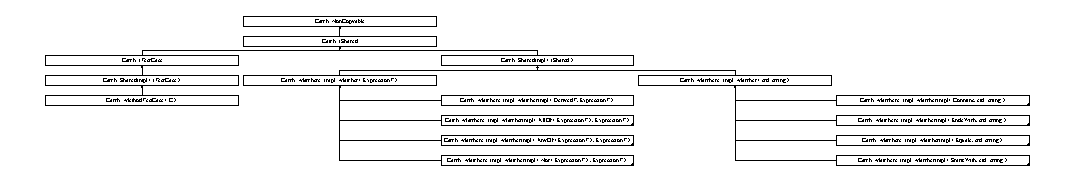
\includegraphics[height=2.004474cm]{structCatch_1_1IShared}
\end{center}
\end{figure}
\subsection*{Public Member Functions}
\begin{DoxyCompactItemize}
\item 
virtual void {\bfseries add\+Ref} () const  =0\hypertarget{structCatch_1_1IShared_ade3e1cd5df74b030058e201ffec156e5}{}\label{structCatch_1_1IShared_ade3e1cd5df74b030058e201ffec156e5}

\item 
virtual void {\bfseries release} () const  =0\hypertarget{structCatch_1_1IShared_a42030b50ca8aa628b48a37e51dd55d29}{}\label{structCatch_1_1IShared_a42030b50ca8aa628b48a37e51dd55d29}

\end{DoxyCompactItemize}


The documentation for this struct was generated from the following file\+:\begin{DoxyCompactItemize}
\item 
catch.\+hpp\end{DoxyCompactItemize}

\hypertarget{structCatch_1_1Detail_1_1IsStreamInsertable}{}\section{Catch\+:\+:Detail\+:\+:Is\+Stream\+Insertable$<$ T $>$ Struct Template Reference}
\label{structCatch_1_1Detail_1_1IsStreamInsertable}\index{Catch\+::\+Detail\+::\+Is\+Stream\+Insertable$<$ T $>$@{Catch\+::\+Detail\+::\+Is\+Stream\+Insertable$<$ T $>$}}
\subsection*{Public Types}
\begin{DoxyCompactItemize}
\item 
enum \{ {\bfseries value} = sizeof( test\+Streamable(s $<$$<$ t) ) == sizeof( True\+Type )
 \}\hypertarget{structCatch_1_1Detail_1_1IsStreamInsertable_a2e4508694da3bf368ff67733a7970edd}{}\label{structCatch_1_1Detail_1_1IsStreamInsertable_a2e4508694da3bf368ff67733a7970edd}

\end{DoxyCompactItemize}
\subsection*{Static Public Attributes}
\begin{DoxyCompactItemize}
\item 
static std\+::ostream \& {\bfseries s}\hypertarget{structCatch_1_1Detail_1_1IsStreamInsertable_abe3d3c8e5d85665747faafffc9a96b00}{}\label{structCatch_1_1Detail_1_1IsStreamInsertable_abe3d3c8e5d85665747faafffc9a96b00}

\item 
static T const \& {\bfseries t}\hypertarget{structCatch_1_1Detail_1_1IsStreamInsertable_a7d2a3da978b6736667a7b2f6d51f507f}{}\label{structCatch_1_1Detail_1_1IsStreamInsertable_a7d2a3da978b6736667a7b2f6d51f507f}

\end{DoxyCompactItemize}


The documentation for this struct was generated from the following file\+:\begin{DoxyCompactItemize}
\item 
catch.\+hpp\end{DoxyCompactItemize}

\hypertarget{structCatch_1_1ITagAliasRegistry}{}\section{Catch\+:\+:I\+Tag\+Alias\+Registry Struct Reference}
\label{structCatch_1_1ITagAliasRegistry}\index{Catch\+::\+I\+Tag\+Alias\+Registry@{Catch\+::\+I\+Tag\+Alias\+Registry}}
\subsection*{Public Member Functions}
\begin{DoxyCompactItemize}
\item 
virtual \hyperlink{classCatch_1_1Option}{Option}$<$ \hyperlink{structCatch_1_1TagAlias}{Tag\+Alias} $>$ {\bfseries find} (std\+::string const \&alias) const  =0\hypertarget{structCatch_1_1ITagAliasRegistry_ad632d35cd51f123d1dbf667e1a8a0d65}{}\label{structCatch_1_1ITagAliasRegistry_ad632d35cd51f123d1dbf667e1a8a0d65}

\item 
virtual std\+::string {\bfseries expand\+Aliases} (std\+::string const \&unexpanded\+Test\+Spec) const  =0\hypertarget{structCatch_1_1ITagAliasRegistry_a2074875f376ff60fb52e7db80421b09c}{}\label{structCatch_1_1ITagAliasRegistry_a2074875f376ff60fb52e7db80421b09c}

\end{DoxyCompactItemize}
\subsection*{Static Public Member Functions}
\begin{DoxyCompactItemize}
\item 
static \hyperlink{structCatch_1_1ITagAliasRegistry}{I\+Tag\+Alias\+Registry} const \& {\bfseries get} ()\hypertarget{structCatch_1_1ITagAliasRegistry_aa9d0f008f49473389c7abf6071f137a7}{}\label{structCatch_1_1ITagAliasRegistry_aa9d0f008f49473389c7abf6071f137a7}

\end{DoxyCompactItemize}


The documentation for this struct was generated from the following file\+:\begin{DoxyCompactItemize}
\item 
catch.\+hpp\end{DoxyCompactItemize}

\hypertarget{structCatch_1_1ITestCase}{}\section{Catch\+:\+:I\+Test\+Case Struct Reference}
\label{structCatch_1_1ITestCase}\index{Catch\+::\+I\+Test\+Case@{Catch\+::\+I\+Test\+Case}}
Inheritance diagram for Catch\+:\+:I\+Test\+Case\+:\begin{figure}[H]
\begin{center}
\leavevmode
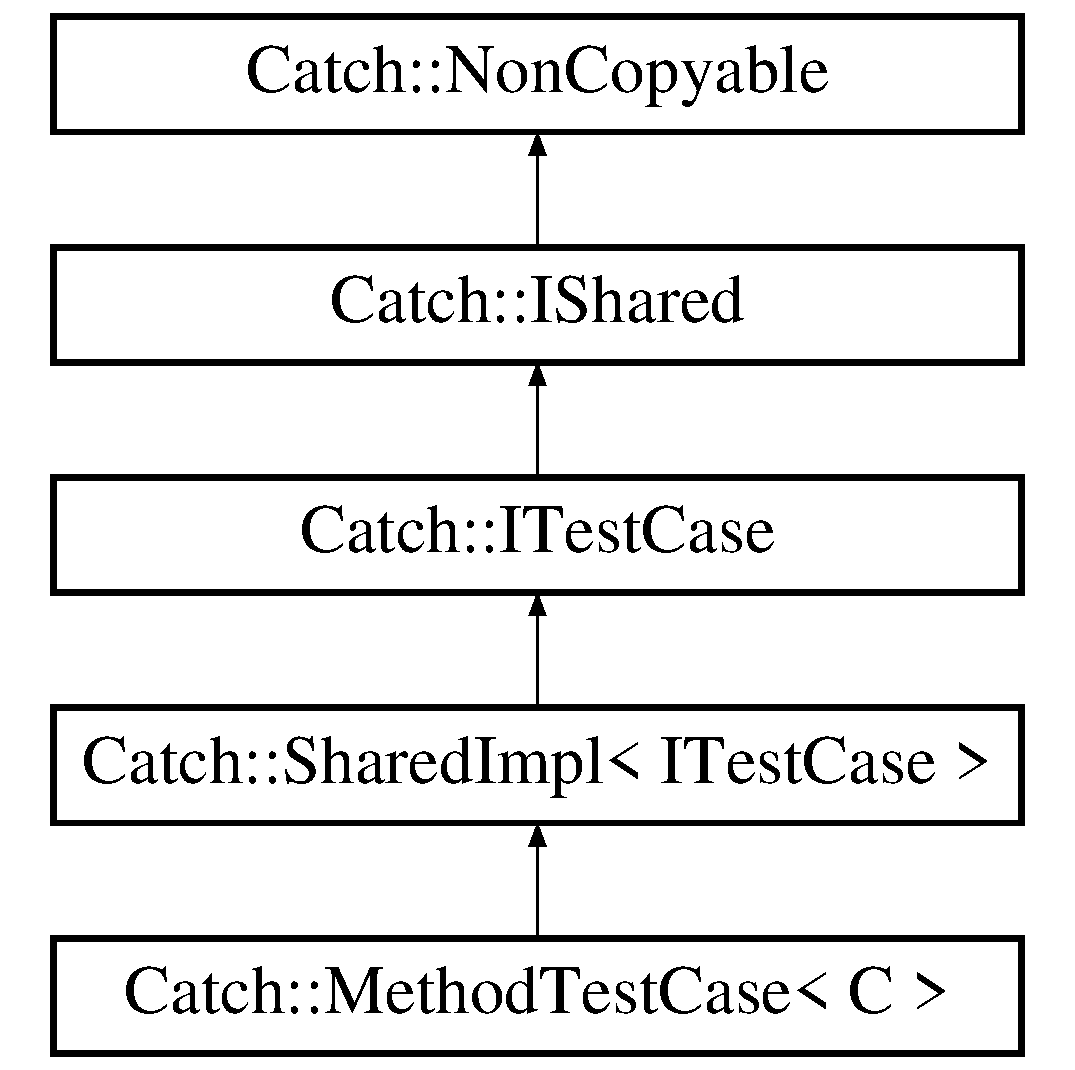
\includegraphics[height=5.000000cm]{structCatch_1_1ITestCase}
\end{center}
\end{figure}
\subsection*{Public Member Functions}
\begin{DoxyCompactItemize}
\item 
virtual void {\bfseries invoke} () const  =0\hypertarget{structCatch_1_1ITestCase_a12b8a2e0140ae975484ec3e96b22b586}{}\label{structCatch_1_1ITestCase_a12b8a2e0140ae975484ec3e96b22b586}

\end{DoxyCompactItemize}


The documentation for this struct was generated from the following file\+:\begin{DoxyCompactItemize}
\item 
catch.\+hpp\end{DoxyCompactItemize}

\hypertarget{structCatch_1_1ITestCaseRegistry}{}\section{Catch\+:\+:I\+Test\+Case\+Registry Struct Reference}
\label{structCatch_1_1ITestCaseRegistry}\index{Catch\+::\+I\+Test\+Case\+Registry@{Catch\+::\+I\+Test\+Case\+Registry}}
\subsection*{Public Member Functions}
\begin{DoxyCompactItemize}
\item 
virtual std\+::vector$<$ \hyperlink{classCatch_1_1TestCase}{Test\+Case} $>$ const \& {\bfseries get\+All\+Tests} () const  =0\hypertarget{structCatch_1_1ITestCaseRegistry_a9c477b3e1ce31c8dbad62e5c6ee146d1}{}\label{structCatch_1_1ITestCaseRegistry_a9c477b3e1ce31c8dbad62e5c6ee146d1}

\item 
virtual std\+::vector$<$ \hyperlink{classCatch_1_1TestCase}{Test\+Case} $>$ const \& {\bfseries get\+All\+Tests\+Sorted} (I\+Config const \&config) const  =0\hypertarget{structCatch_1_1ITestCaseRegistry_ad513b04dfeb0f9c5f7e9657653e86b35}{}\label{structCatch_1_1ITestCaseRegistry_ad513b04dfeb0f9c5f7e9657653e86b35}

\end{DoxyCompactItemize}


The documentation for this struct was generated from the following file\+:\begin{DoxyCompactItemize}
\item 
catch.\+hpp\end{DoxyCompactItemize}

\hypertarget{structCatch_1_1Matchers_1_1Impl_1_1Matcher}{}\section{Catch\+:\+:Matchers\+:\+:Impl\+:\+:Matcher$<$ ExpressionT $>$ Struct Template Reference}
\label{structCatch_1_1Matchers_1_1Impl_1_1Matcher}\index{Catch\+::\+Matchers\+::\+Impl\+::\+Matcher$<$ Expression\+T $>$@{Catch\+::\+Matchers\+::\+Impl\+::\+Matcher$<$ Expression\+T $>$}}
Inheritance diagram for Catch\+:\+:Matchers\+:\+:Impl\+:\+:Matcher$<$ ExpressionT $>$\+:\begin{figure}[H]
\begin{center}
\leavevmode
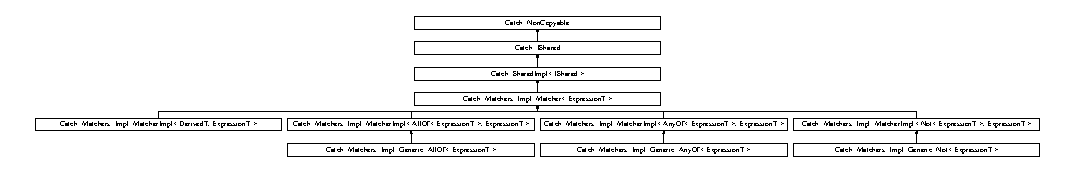
\includegraphics[height=1.879195cm]{structCatch_1_1Matchers_1_1Impl_1_1Matcher}
\end{center}
\end{figure}
\subsection*{Public Types}
\begin{DoxyCompactItemize}
\item 
typedef ExpressionT {\bfseries Expression\+Type}\hypertarget{structCatch_1_1Matchers_1_1Impl_1_1Matcher_a7f5068cbacd1eed06cf243e63446e7e1}{}\label{structCatch_1_1Matchers_1_1Impl_1_1Matcher_a7f5068cbacd1eed06cf243e63446e7e1}

\end{DoxyCompactItemize}
\subsection*{Public Member Functions}
\begin{DoxyCompactItemize}
\item 
virtual \hyperlink{classCatch_1_1Ptr}{Ptr}$<$ \hyperlink{structCatch_1_1Matchers_1_1Impl_1_1Matcher}{Matcher} $>$ {\bfseries clone} () const  =0\hypertarget{structCatch_1_1Matchers_1_1Impl_1_1Matcher_a72c896b9afa03c7e6ac19a0c1d5a634b}{}\label{structCatch_1_1Matchers_1_1Impl_1_1Matcher_a72c896b9afa03c7e6ac19a0c1d5a634b}

\item 
virtual bool {\bfseries match} (ExpressionT const \&expr) const  =0\hypertarget{structCatch_1_1Matchers_1_1Impl_1_1Matcher_a5c00e663b7b83cbf2e4b3d13d9193309}{}\label{structCatch_1_1Matchers_1_1Impl_1_1Matcher_a5c00e663b7b83cbf2e4b3d13d9193309}

\item 
virtual std\+::string {\bfseries to\+String} () const  =0\hypertarget{structCatch_1_1Matchers_1_1Impl_1_1Matcher_afd2469dc5c1869d67d4ad00d3b6388eb}{}\label{structCatch_1_1Matchers_1_1Impl_1_1Matcher_afd2469dc5c1869d67d4ad00d3b6388eb}

\item 
\hyperlink{classCatch_1_1Matchers_1_1Impl_1_1Generic_1_1AllOf}{Generic\+::\+All\+Of}$<$ ExpressionT $>$ {\bfseries operator\&\&} (\hyperlink{structCatch_1_1Matchers_1_1Impl_1_1Matcher}{Matcher}$<$ ExpressionT $>$ const \&other) const \hypertarget{structCatch_1_1Matchers_1_1Impl_1_1Matcher_a1d3b73f684611a6a71396caf74427287}{}\label{structCatch_1_1Matchers_1_1Impl_1_1Matcher_a1d3b73f684611a6a71396caf74427287}

\item 
\hyperlink{classCatch_1_1Matchers_1_1Impl_1_1Generic_1_1AnyOf}{Generic\+::\+Any\+Of}$<$ ExpressionT $>$ {\bfseries operator$\vert$$\vert$} (\hyperlink{structCatch_1_1Matchers_1_1Impl_1_1Matcher}{Matcher}$<$ ExpressionT $>$ const \&other) const \hypertarget{structCatch_1_1Matchers_1_1Impl_1_1Matcher_a2e163b264811ba76638469b537467f9e}{}\label{structCatch_1_1Matchers_1_1Impl_1_1Matcher_a2e163b264811ba76638469b537467f9e}

\item 
\hyperlink{classCatch_1_1Matchers_1_1Impl_1_1Generic_1_1Not}{Generic\+::\+Not}$<$ ExpressionT $>$ {\bfseries operator!} () const \hypertarget{structCatch_1_1Matchers_1_1Impl_1_1Matcher_a534857633dde84924993b674cb248c8f}{}\label{structCatch_1_1Matchers_1_1Impl_1_1Matcher_a534857633dde84924993b674cb248c8f}

\end{DoxyCompactItemize}
\subsection*{Additional Inherited Members}


The documentation for this struct was generated from the following file\+:\begin{DoxyCompactItemize}
\item 
catch.\+hpp\end{DoxyCompactItemize}

\hypertarget{structCatch_1_1Matchers_1_1Impl_1_1MatcherImpl}{}\section{Catch\+:\+:Matchers\+:\+:Impl\+:\+:Matcher\+Impl$<$ DerivedT, ExpressionT $>$ Struct Template Reference}
\label{structCatch_1_1Matchers_1_1Impl_1_1MatcherImpl}\index{Catch\+::\+Matchers\+::\+Impl\+::\+Matcher\+Impl$<$ Derived\+T, Expression\+T $>$@{Catch\+::\+Matchers\+::\+Impl\+::\+Matcher\+Impl$<$ Derived\+T, Expression\+T $>$}}
Inheritance diagram for Catch\+:\+:Matchers\+:\+:Impl\+:\+:Matcher\+Impl$<$ DerivedT, ExpressionT $>$\+:\begin{figure}[H]
\begin{center}
\leavevmode
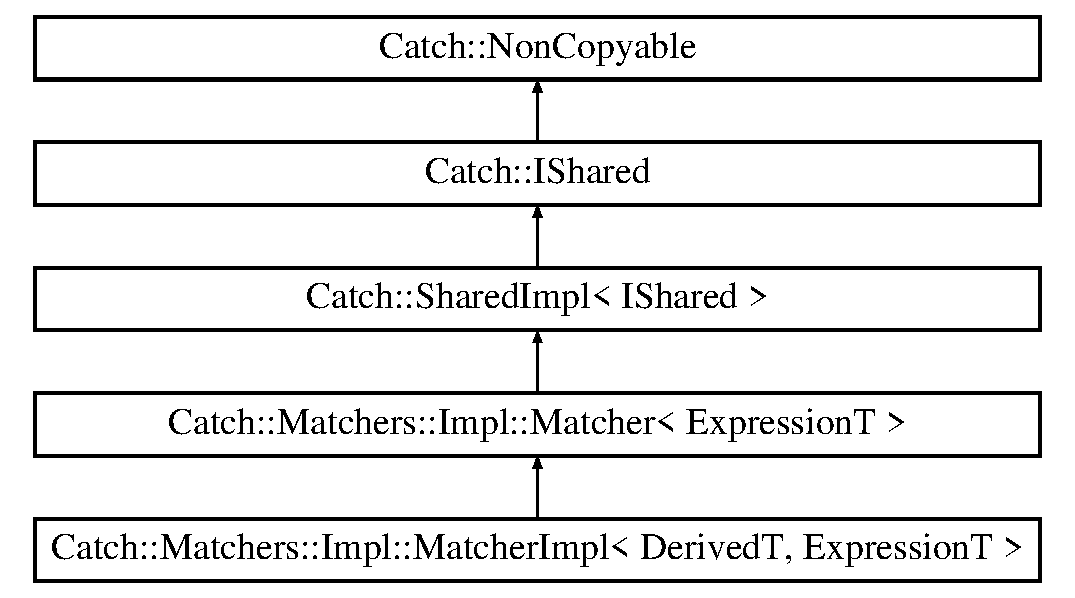
\includegraphics[height=5.000000cm]{structCatch_1_1Matchers_1_1Impl_1_1MatcherImpl}
\end{center}
\end{figure}
\subsection*{Public Member Functions}
\begin{DoxyCompactItemize}
\item 
virtual \hyperlink{classCatch_1_1Ptr}{Ptr}$<$ \hyperlink{structCatch_1_1Matchers_1_1Impl_1_1Matcher}{Matcher}$<$ ExpressionT $>$ $>$ {\bfseries clone} () const \hypertarget{structCatch_1_1Matchers_1_1Impl_1_1MatcherImpl_afe2e10779f91394f80ff5c894fb1bfab}{}\label{structCatch_1_1Matchers_1_1Impl_1_1MatcherImpl_afe2e10779f91394f80ff5c894fb1bfab}

\end{DoxyCompactItemize}
\subsection*{Additional Inherited Members}


The documentation for this struct was generated from the following file\+:\begin{DoxyCompactItemize}
\item 
catch.\+hpp\end{DoxyCompactItemize}

\hypertarget{structCatch_1_1MessageBuilder}{}\section{Catch\+:\+:Message\+Builder Struct Reference}
\label{structCatch_1_1MessageBuilder}\index{Catch\+::\+Message\+Builder@{Catch\+::\+Message\+Builder}}
\subsection*{Public Member Functions}
\begin{DoxyCompactItemize}
\item 
{\bfseries Message\+Builder} (std\+::string const \&macro\+Name, \hyperlink{structCatch_1_1SourceLineInfo}{Source\+Line\+Info} const \&line\+Info, Result\+Was\+::\+Of\+Type type)\hypertarget{structCatch_1_1MessageBuilder_ab0c6378e722680bf58852c6ee2b6e724}{}\label{structCatch_1_1MessageBuilder_ab0c6378e722680bf58852c6ee2b6e724}

\item 
{\footnotesize template$<$typename T $>$ }\\\hyperlink{structCatch_1_1MessageBuilder}{Message\+Builder} \& {\bfseries operator$<$$<$} (T const \&value)\hypertarget{structCatch_1_1MessageBuilder_a20fa48d069b20dddcc2d3df8abb123c1}{}\label{structCatch_1_1MessageBuilder_a20fa48d069b20dddcc2d3df8abb123c1}

\end{DoxyCompactItemize}
\subsection*{Public Attributes}
\begin{DoxyCompactItemize}
\item 
\hyperlink{structCatch_1_1MessageInfo}{Message\+Info} {\bfseries m\+\_\+info}\hypertarget{structCatch_1_1MessageBuilder_a979f1c2b36d78f80ee275bfa5ba0209f}{}\label{structCatch_1_1MessageBuilder_a979f1c2b36d78f80ee275bfa5ba0209f}

\item 
std\+::ostringstream {\bfseries m\+\_\+stream}\hypertarget{structCatch_1_1MessageBuilder_a6488ab0cc4ea52affc9c0612c7c5df6b}{}\label{structCatch_1_1MessageBuilder_a6488ab0cc4ea52affc9c0612c7c5df6b}

\end{DoxyCompactItemize}


The documentation for this struct was generated from the following file\+:\begin{DoxyCompactItemize}
\item 
catch.\+hpp\end{DoxyCompactItemize}

\hypertarget{structCatch_1_1MessageInfo}{}\section{Catch\+:\+:Message\+Info Struct Reference}
\label{structCatch_1_1MessageInfo}\index{Catch\+::\+Message\+Info@{Catch\+::\+Message\+Info}}
\subsection*{Public Member Functions}
\begin{DoxyCompactItemize}
\item 
{\bfseries Message\+Info} (std\+::string const \&\+\_\+macro\+Name, \hyperlink{structCatch_1_1SourceLineInfo}{Source\+Line\+Info} const \&\+\_\+line\+Info, Result\+Was\+::\+Of\+Type \+\_\+type)\hypertarget{structCatch_1_1MessageInfo_a2e336c33ebef7af3c1bbae6a56e14f8a}{}\label{structCatch_1_1MessageInfo_a2e336c33ebef7af3c1bbae6a56e14f8a}

\item 
bool {\bfseries operator==} (\hyperlink{structCatch_1_1MessageInfo}{Message\+Info} const \&other) const \hypertarget{structCatch_1_1MessageInfo_a30fe117138e568c5a9dfdabb7de6e790}{}\label{structCatch_1_1MessageInfo_a30fe117138e568c5a9dfdabb7de6e790}

\item 
bool {\bfseries operator$<$} (\hyperlink{structCatch_1_1MessageInfo}{Message\+Info} const \&other) const \hypertarget{structCatch_1_1MessageInfo_a7a2b1ec3772cd35176e2ee25a94be16a}{}\label{structCatch_1_1MessageInfo_a7a2b1ec3772cd35176e2ee25a94be16a}

\end{DoxyCompactItemize}
\subsection*{Public Attributes}
\begin{DoxyCompactItemize}
\item 
std\+::string {\bfseries macro\+Name}\hypertarget{structCatch_1_1MessageInfo_a156ade4b3cc731f6ec7b542ae47ba8e3}{}\label{structCatch_1_1MessageInfo_a156ade4b3cc731f6ec7b542ae47ba8e3}

\item 
\hyperlink{structCatch_1_1SourceLineInfo}{Source\+Line\+Info} {\bfseries line\+Info}\hypertarget{structCatch_1_1MessageInfo_a985165328723e599696ebd8e43195cc5}{}\label{structCatch_1_1MessageInfo_a985165328723e599696ebd8e43195cc5}

\item 
Result\+Was\+::\+Of\+Type {\bfseries type}\hypertarget{structCatch_1_1MessageInfo_ae928b9117465c696e45951d9d0284e78}{}\label{structCatch_1_1MessageInfo_ae928b9117465c696e45951d9d0284e78}

\item 
std\+::string {\bfseries message}\hypertarget{structCatch_1_1MessageInfo_ab6cd06e050bf426c6577502a5c50e256}{}\label{structCatch_1_1MessageInfo_ab6cd06e050bf426c6577502a5c50e256}

\item 
unsigned int {\bfseries sequence}\hypertarget{structCatch_1_1MessageInfo_a7f4f57ea21e50160adefce7b68a781d6}{}\label{structCatch_1_1MessageInfo_a7f4f57ea21e50160adefce7b68a781d6}

\end{DoxyCompactItemize}


The documentation for this struct was generated from the following file\+:\begin{DoxyCompactItemize}
\item 
catch.\+hpp\end{DoxyCompactItemize}

\hypertarget{classCatch_1_1MethodTestCase}{}\section{Catch\+:\+:Method\+Test\+Case$<$ C $>$ Class Template Reference}
\label{classCatch_1_1MethodTestCase}\index{Catch\+::\+Method\+Test\+Case$<$ C $>$@{Catch\+::\+Method\+Test\+Case$<$ C $>$}}
Inheritance diagram for Catch\+:\+:Method\+Test\+Case$<$ C $>$\+:\begin{figure}[H]
\begin{center}
\leavevmode
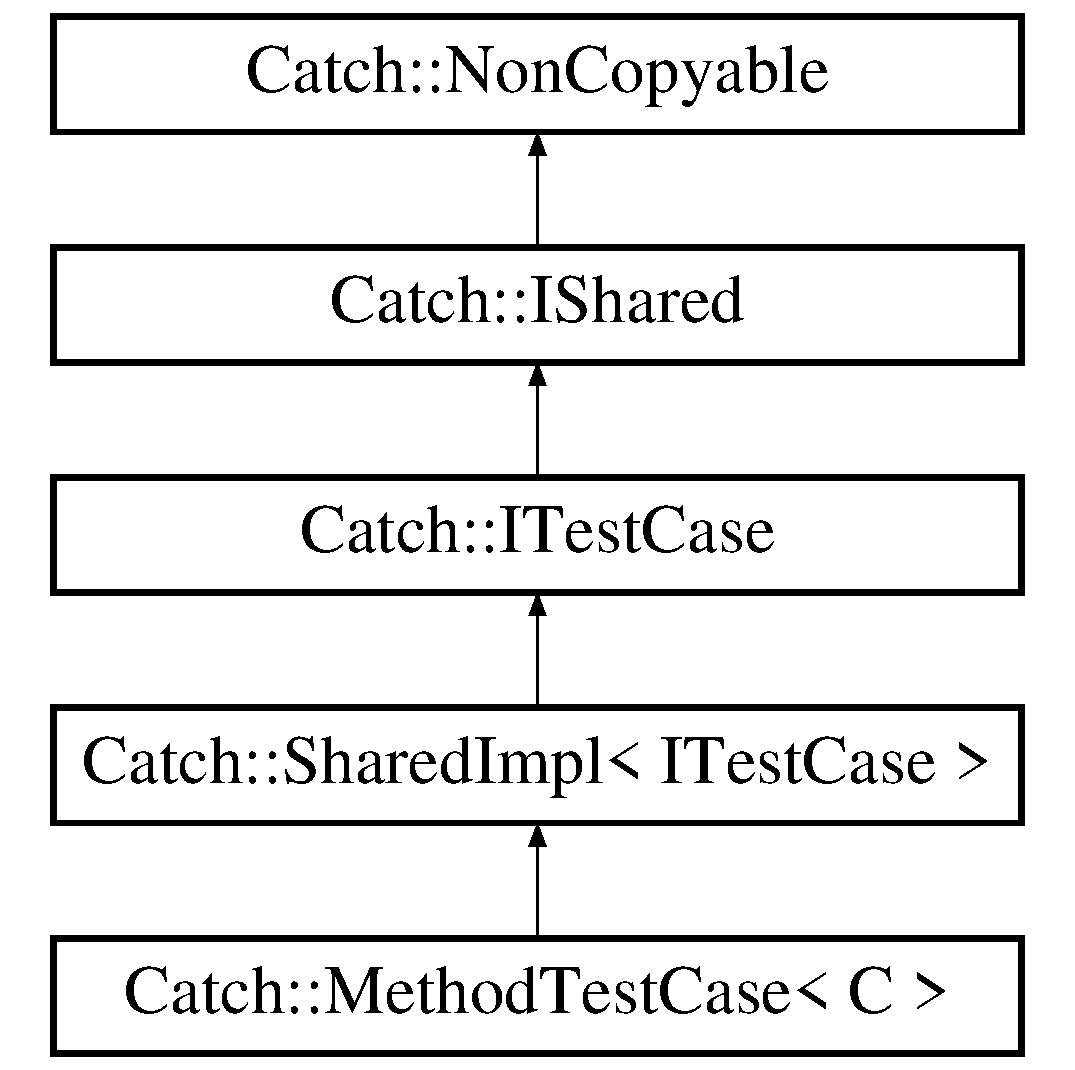
\includegraphics[height=5.000000cm]{classCatch_1_1MethodTestCase}
\end{center}
\end{figure}
\subsection*{Public Member Functions}
\begin{DoxyCompactItemize}
\item 
{\bfseries Method\+Test\+Case} (void(C\+::$\ast$method)())\hypertarget{classCatch_1_1MethodTestCase_a7b043b85dae371358255dd9dc6582e7b}{}\label{classCatch_1_1MethodTestCase_a7b043b85dae371358255dd9dc6582e7b}

\item 
virtual void {\bfseries invoke} () const \hypertarget{classCatch_1_1MethodTestCase_a39cc4b760dd71adc3f7550bc1e7eb697}{}\label{classCatch_1_1MethodTestCase_a39cc4b760dd71adc3f7550bc1e7eb697}

\end{DoxyCompactItemize}
\subsection*{Additional Inherited Members}


The documentation for this class was generated from the following file\+:\begin{DoxyCompactItemize}
\item 
catch.\+hpp\end{DoxyCompactItemize}

\hypertarget{structCatch_1_1NameAndDesc}{}\section{Catch\+:\+:Name\+And\+Desc Struct Reference}
\label{structCatch_1_1NameAndDesc}\index{Catch\+::\+Name\+And\+Desc@{Catch\+::\+Name\+And\+Desc}}
\subsection*{Public Member Functions}
\begin{DoxyCompactItemize}
\item 
{\bfseries Name\+And\+Desc} (const char $\ast$\+\_\+name=\char`\"{}\char`\"{}, const char $\ast$\+\_\+description=\char`\"{}\char`\"{})\hypertarget{structCatch_1_1NameAndDesc_a189ceb9942fb5f6635140d6a09fc843a}{}\label{structCatch_1_1NameAndDesc_a189ceb9942fb5f6635140d6a09fc843a}

\end{DoxyCompactItemize}
\subsection*{Public Attributes}
\begin{DoxyCompactItemize}
\item 
const char $\ast$ {\bfseries name}\hypertarget{structCatch_1_1NameAndDesc_a374b4ed8be3cf98be20ebde5273bde51}{}\label{structCatch_1_1NameAndDesc_a374b4ed8be3cf98be20ebde5273bde51}

\item 
const char $\ast$ {\bfseries description}\hypertarget{structCatch_1_1NameAndDesc_a3463a23ff65ce494fc380452b57b7970}{}\label{structCatch_1_1NameAndDesc_a3463a23ff65ce494fc380452b57b7970}

\end{DoxyCompactItemize}


The documentation for this struct was generated from the following file\+:\begin{DoxyCompactItemize}
\item 
catch.\+hpp\end{DoxyCompactItemize}

\hypertarget{classCatch_1_1NonCopyable}{}\section{Catch\+:\+:Non\+Copyable Class Reference}
\label{classCatch_1_1NonCopyable}\index{Catch\+::\+Non\+Copyable@{Catch\+::\+Non\+Copyable}}
Inheritance diagram for Catch\+:\+:Non\+Copyable\+:\begin{figure}[H]
\begin{center}
\leavevmode
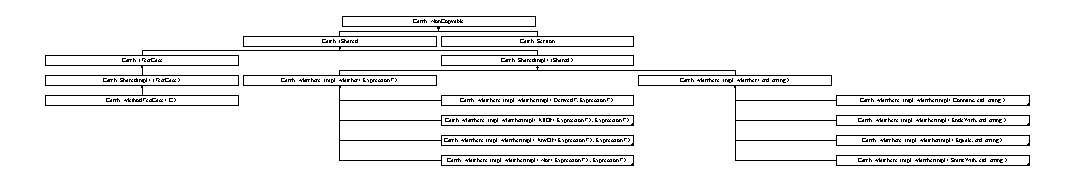
\includegraphics[height=2.004474cm]{classCatch_1_1NonCopyable}
\end{center}
\end{figure}


The documentation for this class was generated from the following file\+:\begin{DoxyCompactItemize}
\item 
catch.\+hpp\end{DoxyCompactItemize}

\hypertarget{classCatch_1_1Matchers_1_1Impl_1_1Generic_1_1Not}{}\section{Catch\+:\+:Matchers\+:\+:Impl\+:\+:Generic\+:\+:Not$<$ ExpressionT $>$ Class Template Reference}
\label{classCatch_1_1Matchers_1_1Impl_1_1Generic_1_1Not}\index{Catch\+::\+Matchers\+::\+Impl\+::\+Generic\+::\+Not$<$ Expression\+T $>$@{Catch\+::\+Matchers\+::\+Impl\+::\+Generic\+::\+Not$<$ Expression\+T $>$}}
Inheritance diagram for Catch\+:\+:Matchers\+:\+:Impl\+:\+:Generic\+:\+:Not$<$ ExpressionT $>$\+:\begin{figure}[H]
\begin{center}
\leavevmode
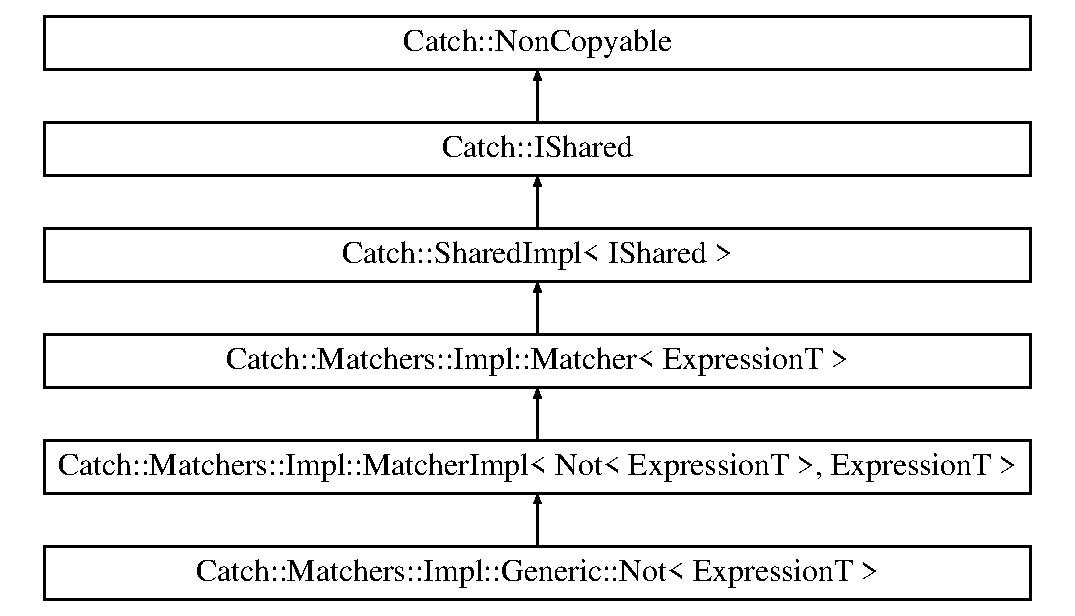
\includegraphics[height=6.000000cm]{classCatch_1_1Matchers_1_1Impl_1_1Generic_1_1Not}
\end{center}
\end{figure}
\subsection*{Public Member Functions}
\begin{DoxyCompactItemize}
\item 
{\bfseries Not} (\hyperlink{structCatch_1_1Matchers_1_1Impl_1_1Matcher}{Matcher}$<$ ExpressionT $>$ const \&matcher)\hypertarget{classCatch_1_1Matchers_1_1Impl_1_1Generic_1_1Not_a9b99e3ce49c1a16931708b67c312f204}{}\label{classCatch_1_1Matchers_1_1Impl_1_1Generic_1_1Not_a9b99e3ce49c1a16931708b67c312f204}

\item 
{\bfseries Not} (\hyperlink{classCatch_1_1Matchers_1_1Impl_1_1Generic_1_1Not}{Not} const \&other)\hypertarget{classCatch_1_1Matchers_1_1Impl_1_1Generic_1_1Not_a46eccbbaeec259d3536aa2a29f95208f}{}\label{classCatch_1_1Matchers_1_1Impl_1_1Generic_1_1Not_a46eccbbaeec259d3536aa2a29f95208f}

\item 
virtual bool {\bfseries match} (ExpressionT const \&expr) const C\+A\+T\+C\+H\+\_\+\+O\+V\+E\+R\+R\+I\+DE\hypertarget{classCatch_1_1Matchers_1_1Impl_1_1Generic_1_1Not_a18c49fc6fb73a42d54650dafc18c7db1}{}\label{classCatch_1_1Matchers_1_1Impl_1_1Generic_1_1Not_a18c49fc6fb73a42d54650dafc18c7db1}

\item 
virtual std\+::string {\bfseries to\+String} () const C\+A\+T\+C\+H\+\_\+\+O\+V\+E\+R\+R\+I\+DE\hypertarget{classCatch_1_1Matchers_1_1Impl_1_1Generic_1_1Not_ab970a4a6e58a987451e0b0e0e60a0bff}{}\label{classCatch_1_1Matchers_1_1Impl_1_1Generic_1_1Not_ab970a4a6e58a987451e0b0e0e60a0bff}

\end{DoxyCompactItemize}
\subsection*{Additional Inherited Members}


The documentation for this class was generated from the following file\+:\begin{DoxyCompactItemize}
\item 
catch.\+hpp\end{DoxyCompactItemize}

\hypertarget{classCatch_1_1NotImplementedException}{}\section{Catch\+:\+:Not\+Implemented\+Exception Class Reference}
\label{classCatch_1_1NotImplementedException}\index{Catch\+::\+Not\+Implemented\+Exception@{Catch\+::\+Not\+Implemented\+Exception}}
Inheritance diagram for Catch\+:\+:Not\+Implemented\+Exception\+:\begin{figure}[H]
\begin{center}
\leavevmode
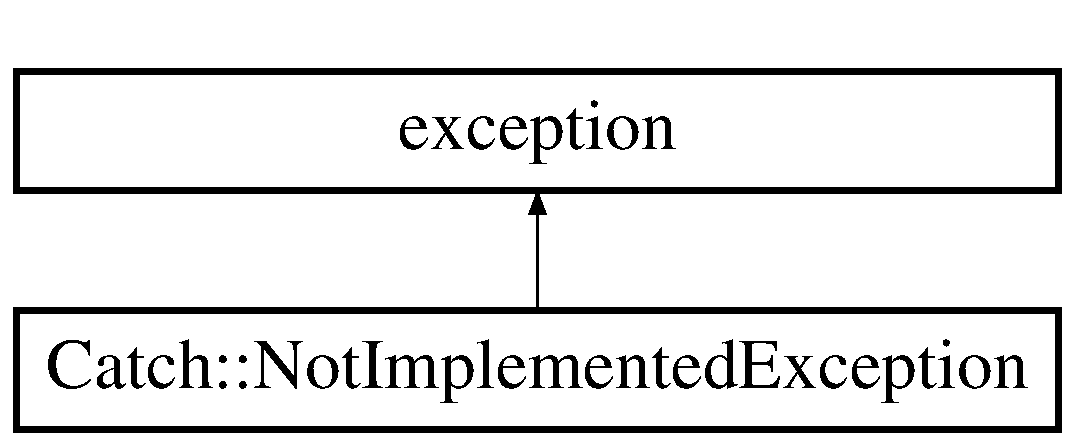
\includegraphics[height=2.000000cm]{classCatch_1_1NotImplementedException}
\end{center}
\end{figure}
\subsection*{Public Member Functions}
\begin{DoxyCompactItemize}
\item 
{\bfseries Not\+Implemented\+Exception} (\hyperlink{structCatch_1_1SourceLineInfo}{Source\+Line\+Info} const \&line\+Info)\hypertarget{classCatch_1_1NotImplementedException_ab4f0a5c39d8ffb72c664e2c07e180634}{}\label{classCatch_1_1NotImplementedException_ab4f0a5c39d8ffb72c664e2c07e180634}

\item 
{\bfseries Not\+Implemented\+Exception} (\hyperlink{classCatch_1_1NotImplementedException}{Not\+Implemented\+Exception} const \&)\hypertarget{classCatch_1_1NotImplementedException_a508a7a833455da2d3c10ea1a9d45e982}{}\label{classCatch_1_1NotImplementedException_a508a7a833455da2d3c10ea1a9d45e982}

\item 
virtual const char $\ast$ {\bfseries what} () const C\+A\+T\+C\+H\+\_\+\+N\+O\+E\+X\+C\+E\+PT\hypertarget{classCatch_1_1NotImplementedException_ad4c13963f1a8feacda0cd331adda89e3}{}\label{classCatch_1_1NotImplementedException_ad4c13963f1a8feacda0cd331adda89e3}

\end{DoxyCompactItemize}


The documentation for this class was generated from the following file\+:\begin{DoxyCompactItemize}
\item 
catch.\+hpp\end{DoxyCompactItemize}

\hypertarget{structCatch_1_1Internal_1_1OperatorTraits}{}\section{Catch\+:\+:Internal\+:\+:Operator\+Traits$<$ Op $>$ Struct Template Reference}
\label{structCatch_1_1Internal_1_1OperatorTraits}\index{Catch\+::\+Internal\+::\+Operator\+Traits$<$ Op $>$@{Catch\+::\+Internal\+::\+Operator\+Traits$<$ Op $>$}}
\subsection*{Static Public Member Functions}
\begin{DoxyCompactItemize}
\item 
static const char $\ast$ {\bfseries get\+Name} ()\hypertarget{structCatch_1_1Internal_1_1OperatorTraits_ac6d08082ea33348d42bc4ccbd6d07671}{}\label{structCatch_1_1Internal_1_1OperatorTraits_ac6d08082ea33348d42bc4ccbd6d07671}

\end{DoxyCompactItemize}


The documentation for this struct was generated from the following file\+:\begin{DoxyCompactItemize}
\item 
catch.\+hpp\end{DoxyCompactItemize}

\hypertarget{structCatch_1_1Internal_1_1OperatorTraits_3_01IsEqualTo_01_4}{}\section{Catch\+:\+:Internal\+:\+:Operator\+Traits$<$ Is\+Equal\+To $>$ Struct Template Reference}
\label{structCatch_1_1Internal_1_1OperatorTraits_3_01IsEqualTo_01_4}\index{Catch\+::\+Internal\+::\+Operator\+Traits$<$ Is\+Equal\+To $>$@{Catch\+::\+Internal\+::\+Operator\+Traits$<$ Is\+Equal\+To $>$}}
\subsection*{Static Public Member Functions}
\begin{DoxyCompactItemize}
\item 
static const char $\ast$ {\bfseries get\+Name} ()\hypertarget{structCatch_1_1Internal_1_1OperatorTraits_3_01IsEqualTo_01_4_addf03ac66f0ed83abcc037a7a327d4f1}{}\label{structCatch_1_1Internal_1_1OperatorTraits_3_01IsEqualTo_01_4_addf03ac66f0ed83abcc037a7a327d4f1}

\end{DoxyCompactItemize}


The documentation for this struct was generated from the following file\+:\begin{DoxyCompactItemize}
\item 
catch.\+hpp\end{DoxyCompactItemize}

\hypertarget{structCatch_1_1Internal_1_1OperatorTraits_3_01IsGreaterThan_01_4}{}\section{Catch\+:\+:Internal\+:\+:Operator\+Traits$<$ Is\+Greater\+Than $>$ Struct Template Reference}
\label{structCatch_1_1Internal_1_1OperatorTraits_3_01IsGreaterThan_01_4}\index{Catch\+::\+Internal\+::\+Operator\+Traits$<$ Is\+Greater\+Than $>$@{Catch\+::\+Internal\+::\+Operator\+Traits$<$ Is\+Greater\+Than $>$}}
\subsection*{Static Public Member Functions}
\begin{DoxyCompactItemize}
\item 
static const char $\ast$ {\bfseries get\+Name} ()\hypertarget{structCatch_1_1Internal_1_1OperatorTraits_3_01IsGreaterThan_01_4_ab917bfb9ccbe461dc684ee5a34d67d27}{}\label{structCatch_1_1Internal_1_1OperatorTraits_3_01IsGreaterThan_01_4_ab917bfb9ccbe461dc684ee5a34d67d27}

\end{DoxyCompactItemize}


The documentation for this struct was generated from the following file\+:\begin{DoxyCompactItemize}
\item 
catch.\+hpp\end{DoxyCompactItemize}

\hypertarget{structCatch_1_1Internal_1_1OperatorTraits_3_01IsGreaterThanOrEqualTo_01_4}{}\section{Catch\+:\+:Internal\+:\+:Operator\+Traits$<$ Is\+Greater\+Than\+Or\+Equal\+To $>$ Struct Template Reference}
\label{structCatch_1_1Internal_1_1OperatorTraits_3_01IsGreaterThanOrEqualTo_01_4}\index{Catch\+::\+Internal\+::\+Operator\+Traits$<$ Is\+Greater\+Than\+Or\+Equal\+To $>$@{Catch\+::\+Internal\+::\+Operator\+Traits$<$ Is\+Greater\+Than\+Or\+Equal\+To $>$}}
\subsection*{Static Public Member Functions}
\begin{DoxyCompactItemize}
\item 
static const char $\ast$ {\bfseries get\+Name} ()\hypertarget{structCatch_1_1Internal_1_1OperatorTraits_3_01IsGreaterThanOrEqualTo_01_4_a76b6f6b0dbaf7d19ebb1b4b4891e719e}{}\label{structCatch_1_1Internal_1_1OperatorTraits_3_01IsGreaterThanOrEqualTo_01_4_a76b6f6b0dbaf7d19ebb1b4b4891e719e}

\end{DoxyCompactItemize}


The documentation for this struct was generated from the following file\+:\begin{DoxyCompactItemize}
\item 
catch.\+hpp\end{DoxyCompactItemize}

\hypertarget{structCatch_1_1Internal_1_1OperatorTraits_3_01IsLessThan_01_4}{}\section{Catch\+:\+:Internal\+:\+:Operator\+Traits$<$ Is\+Less\+Than $>$ Struct Template Reference}
\label{structCatch_1_1Internal_1_1OperatorTraits_3_01IsLessThan_01_4}\index{Catch\+::\+Internal\+::\+Operator\+Traits$<$ Is\+Less\+Than $>$@{Catch\+::\+Internal\+::\+Operator\+Traits$<$ Is\+Less\+Than $>$}}
\subsection*{Static Public Member Functions}
\begin{DoxyCompactItemize}
\item 
static const char $\ast$ {\bfseries get\+Name} ()\hypertarget{structCatch_1_1Internal_1_1OperatorTraits_3_01IsLessThan_01_4_aa3b536ddbd2e34b1253931ff00c32712}{}\label{structCatch_1_1Internal_1_1OperatorTraits_3_01IsLessThan_01_4_aa3b536ddbd2e34b1253931ff00c32712}

\end{DoxyCompactItemize}


The documentation for this struct was generated from the following file\+:\begin{DoxyCompactItemize}
\item 
catch.\+hpp\end{DoxyCompactItemize}

\hypertarget{structCatch_1_1Internal_1_1OperatorTraits_3_01IsLessThanOrEqualTo_01_4}{}\section{Catch\+:\+:Internal\+:\+:Operator\+Traits$<$ Is\+Less\+Than\+Or\+Equal\+To $>$ Struct Template Reference}
\label{structCatch_1_1Internal_1_1OperatorTraits_3_01IsLessThanOrEqualTo_01_4}\index{Catch\+::\+Internal\+::\+Operator\+Traits$<$ Is\+Less\+Than\+Or\+Equal\+To $>$@{Catch\+::\+Internal\+::\+Operator\+Traits$<$ Is\+Less\+Than\+Or\+Equal\+To $>$}}
\subsection*{Static Public Member Functions}
\begin{DoxyCompactItemize}
\item 
static const char $\ast$ {\bfseries get\+Name} ()\hypertarget{structCatch_1_1Internal_1_1OperatorTraits_3_01IsLessThanOrEqualTo_01_4_ae8578813bc847838f10448c1541a9d7b}{}\label{structCatch_1_1Internal_1_1OperatorTraits_3_01IsLessThanOrEqualTo_01_4_ae8578813bc847838f10448c1541a9d7b}

\end{DoxyCompactItemize}


The documentation for this struct was generated from the following file\+:\begin{DoxyCompactItemize}
\item 
catch.\+hpp\end{DoxyCompactItemize}

\hypertarget{structCatch_1_1Internal_1_1OperatorTraits_3_01IsNotEqualTo_01_4}{}\section{Catch\+:\+:Internal\+:\+:Operator\+Traits$<$ Is\+Not\+Equal\+To $>$ Struct Template Reference}
\label{structCatch_1_1Internal_1_1OperatorTraits_3_01IsNotEqualTo_01_4}\index{Catch\+::\+Internal\+::\+Operator\+Traits$<$ Is\+Not\+Equal\+To $>$@{Catch\+::\+Internal\+::\+Operator\+Traits$<$ Is\+Not\+Equal\+To $>$}}
\subsection*{Static Public Member Functions}
\begin{DoxyCompactItemize}
\item 
static const char $\ast$ {\bfseries get\+Name} ()\hypertarget{structCatch_1_1Internal_1_1OperatorTraits_3_01IsNotEqualTo_01_4_a54a795b8bf7c80a9fdbc7b81f39133b4}{}\label{structCatch_1_1Internal_1_1OperatorTraits_3_01IsNotEqualTo_01_4_a54a795b8bf7c80a9fdbc7b81f39133b4}

\end{DoxyCompactItemize}


The documentation for this struct was generated from the following file\+:\begin{DoxyCompactItemize}
\item 
catch.\+hpp\end{DoxyCompactItemize}

\hypertarget{classCatch_1_1Option}{}\section{Catch\+:\+:Option$<$ T $>$ Class Template Reference}
\label{classCatch_1_1Option}\index{Catch\+::\+Option$<$ T $>$@{Catch\+::\+Option$<$ T $>$}}
\subsection*{Public Member Functions}
\begin{DoxyCompactItemize}
\item 
{\bfseries Option} (T const \&\+\_\+value)\hypertarget{classCatch_1_1Option_a5aeb9c22d48a6882bdf5fb4730b06c86}{}\label{classCatch_1_1Option_a5aeb9c22d48a6882bdf5fb4730b06c86}

\item 
{\bfseries Option} (\hyperlink{classCatch_1_1Option}{Option} const \&\+\_\+other)\hypertarget{classCatch_1_1Option_af02f2e4559f06384baec0def8c68c5fd}{}\label{classCatch_1_1Option_af02f2e4559f06384baec0def8c68c5fd}

\item 
\hyperlink{classCatch_1_1Option}{Option} \& {\bfseries operator=} (\hyperlink{classCatch_1_1Option}{Option} const \&\+\_\+other)\hypertarget{classCatch_1_1Option_a78c65b15dd6b2fbd04c5012c43017c8f}{}\label{classCatch_1_1Option_a78c65b15dd6b2fbd04c5012c43017c8f}

\item 
\hyperlink{classCatch_1_1Option}{Option} \& {\bfseries operator=} (T const \&\+\_\+value)\hypertarget{classCatch_1_1Option_a2be7e343ab22d6061726d32ab4622653}{}\label{classCatch_1_1Option_a2be7e343ab22d6061726d32ab4622653}

\item 
void {\bfseries reset} ()\hypertarget{classCatch_1_1Option_a37b4e0e5d4d56296adacd267a616f4e0}{}\label{classCatch_1_1Option_a37b4e0e5d4d56296adacd267a616f4e0}

\item 
T \& {\bfseries operator$\ast$} ()\hypertarget{classCatch_1_1Option_afd989852fa453731c3190dac63caccb0}{}\label{classCatch_1_1Option_afd989852fa453731c3190dac63caccb0}

\item 
T const \& {\bfseries operator$\ast$} () const \hypertarget{classCatch_1_1Option_a0f05708905dc6b0b470fb24f5d265631}{}\label{classCatch_1_1Option_a0f05708905dc6b0b470fb24f5d265631}

\item 
T $\ast$ {\bfseries operator-\/$>$} ()\hypertarget{classCatch_1_1Option_acad340798a16c8f700f8763119e90f31}{}\label{classCatch_1_1Option_acad340798a16c8f700f8763119e90f31}

\item 
const T $\ast$ {\bfseries operator-\/$>$} () const \hypertarget{classCatch_1_1Option_a0800340b2971748671b88acfb14bb928}{}\label{classCatch_1_1Option_a0800340b2971748671b88acfb14bb928}

\item 
T {\bfseries value\+Or} (T const \&default\+Value) const \hypertarget{classCatch_1_1Option_a21b5629a7febbe3e23c475c9d9138a2d}{}\label{classCatch_1_1Option_a21b5629a7febbe3e23c475c9d9138a2d}

\item 
bool {\bfseries some} () const \hypertarget{classCatch_1_1Option_affa96f15798b4656fb753ff52d12dec2}{}\label{classCatch_1_1Option_affa96f15798b4656fb753ff52d12dec2}

\item 
bool {\bfseries none} () const \hypertarget{classCatch_1_1Option_a389324d2aa20ceb0eb0f48a5f77c20c8}{}\label{classCatch_1_1Option_a389324d2aa20ceb0eb0f48a5f77c20c8}

\item 
bool {\bfseries operator!} () const \hypertarget{classCatch_1_1Option_a47a1b6f6def2730ea9d27a1860a4f97f}{}\label{classCatch_1_1Option_a47a1b6f6def2730ea9d27a1860a4f97f}

\item 
{\bfseries operator Safe\+Bool\+::type} () const \hypertarget{classCatch_1_1Option_a637d4366ae7f0ded52ce59c8cb06da7b}{}\label{classCatch_1_1Option_a637d4366ae7f0ded52ce59c8cb06da7b}

\end{DoxyCompactItemize}


The documentation for this class was generated from the following file\+:\begin{DoxyCompactItemize}
\item 
catch.\+hpp\end{DoxyCompactItemize}

\hypertarget{structCatch_1_1pluralise}{}\section{Catch\+:\+:pluralise Struct Reference}
\label{structCatch_1_1pluralise}\index{Catch\+::pluralise@{Catch\+::pluralise}}
\subsection*{Public Member Functions}
\begin{DoxyCompactItemize}
\item 
{\bfseries pluralise} (std\+::size\+\_\+t count, std\+::string const \&label)\hypertarget{structCatch_1_1pluralise_a5c55e22de2416cfe416edf715c6b9234}{}\label{structCatch_1_1pluralise_a5c55e22de2416cfe416edf715c6b9234}

\end{DoxyCompactItemize}
\subsection*{Public Attributes}
\begin{DoxyCompactItemize}
\item 
std\+::size\+\_\+t {\bfseries m\+\_\+count}\hypertarget{structCatch_1_1pluralise_a4dce2fa13ec6f00fac09b2418265441e}{}\label{structCatch_1_1pluralise_a4dce2fa13ec6f00fac09b2418265441e}

\item 
std\+::string {\bfseries m\+\_\+label}\hypertarget{structCatch_1_1pluralise_a8849cbdd3f11ebe7747597c8644e8793}{}\label{structCatch_1_1pluralise_a8849cbdd3f11ebe7747597c8644e8793}

\end{DoxyCompactItemize}
\subsection*{Friends}
\begin{DoxyCompactItemize}
\item 
std\+::ostream \& {\bfseries operator$<$$<$} (std\+::ostream \&os, \hyperlink{structCatch_1_1pluralise}{pluralise} const \&pluraliser)\hypertarget{structCatch_1_1pluralise_aa7dac6b165514c1f85e0695d678fdef5}{}\label{structCatch_1_1pluralise_aa7dac6b165514c1f85e0695d678fdef5}

\end{DoxyCompactItemize}


The documentation for this struct was generated from the following file\+:\begin{DoxyCompactItemize}
\item 
catch.\+hpp\end{DoxyCompactItemize}

\hypertarget{classCatch_1_1Ptr}{}\section{Catch\+:\+:Ptr$<$ T $>$ Class Template Reference}
\label{classCatch_1_1Ptr}\index{Catch\+::\+Ptr$<$ T $>$@{Catch\+::\+Ptr$<$ T $>$}}
\subsection*{Public Member Functions}
\begin{DoxyCompactItemize}
\item 
{\bfseries Ptr} (T $\ast$p)\hypertarget{classCatch_1_1Ptr_aacec063a79cd142e39040a31c6b3c40b}{}\label{classCatch_1_1Ptr_aacec063a79cd142e39040a31c6b3c40b}

\item 
{\bfseries Ptr} (\hyperlink{classCatch_1_1Ptr}{Ptr} const \&other)\hypertarget{classCatch_1_1Ptr_ac629dd8ebe5763a37bb89e6c1d6a1771}{}\label{classCatch_1_1Ptr_ac629dd8ebe5763a37bb89e6c1d6a1771}

\item 
void {\bfseries reset} ()\hypertarget{classCatch_1_1Ptr_af8d0fa7a2cd20842830b354ac31dfe5c}{}\label{classCatch_1_1Ptr_af8d0fa7a2cd20842830b354ac31dfe5c}

\item 
\hyperlink{classCatch_1_1Ptr}{Ptr} \& {\bfseries operator=} (T $\ast$p)\hypertarget{classCatch_1_1Ptr_a9b08c868b447d679ed201921f5c94683}{}\label{classCatch_1_1Ptr_a9b08c868b447d679ed201921f5c94683}

\item 
\hyperlink{classCatch_1_1Ptr}{Ptr} \& {\bfseries operator=} (\hyperlink{classCatch_1_1Ptr}{Ptr} const \&other)\hypertarget{classCatch_1_1Ptr_af42074444c1bc6a70ebdc406a8617708}{}\label{classCatch_1_1Ptr_af42074444c1bc6a70ebdc406a8617708}

\item 
void {\bfseries swap} (\hyperlink{classCatch_1_1Ptr}{Ptr} \&other)\hypertarget{classCatch_1_1Ptr_a172bf8b4e71e26a5a4d92f5b02158b50}{}\label{classCatch_1_1Ptr_a172bf8b4e71e26a5a4d92f5b02158b50}

\item 
T $\ast$ {\bfseries get} () const \hypertarget{classCatch_1_1Ptr_a1617aa5ff058b53ea572cf965617b7ae}{}\label{classCatch_1_1Ptr_a1617aa5ff058b53ea572cf965617b7ae}

\item 
T \& {\bfseries operator$\ast$} () const \hypertarget{classCatch_1_1Ptr_a3a4c139032a8bd1bffa553103d5dbfd3}{}\label{classCatch_1_1Ptr_a3a4c139032a8bd1bffa553103d5dbfd3}

\item 
T $\ast$ {\bfseries operator-\/$>$} () const \hypertarget{classCatch_1_1Ptr_afaa13250d5e0ae5a440726d5e5aa7295}{}\label{classCatch_1_1Ptr_afaa13250d5e0ae5a440726d5e5aa7295}

\item 
bool {\bfseries operator!} () const \hypertarget{classCatch_1_1Ptr_aea1a99ded6d62423ccb9173fab91b56e}{}\label{classCatch_1_1Ptr_aea1a99ded6d62423ccb9173fab91b56e}

\item 
{\bfseries operator Safe\+Bool\+::type} () const \hypertarget{classCatch_1_1Ptr_a27234c04feec43ffe0fd08e045557448}{}\label{classCatch_1_1Ptr_a27234c04feec43ffe0fd08e045557448}

\end{DoxyCompactItemize}


The documentation for this class was generated from the following file\+:\begin{DoxyCompactItemize}
\item 
catch.\+hpp\end{DoxyCompactItemize}

\hypertarget{structCatch_1_1RegistrarForTagAliases}{}\section{Catch\+:\+:Registrar\+For\+Tag\+Aliases Struct Reference}
\label{structCatch_1_1RegistrarForTagAliases}\index{Catch\+::\+Registrar\+For\+Tag\+Aliases@{Catch\+::\+Registrar\+For\+Tag\+Aliases}}
\subsection*{Public Member Functions}
\begin{DoxyCompactItemize}
\item 
{\bfseries Registrar\+For\+Tag\+Aliases} (char const $\ast$alias, char const $\ast$tag, \hyperlink{structCatch_1_1SourceLineInfo}{Source\+Line\+Info} const \&line\+Info)\hypertarget{structCatch_1_1RegistrarForTagAliases_ae4e45830e4763bcd65d55d8db9167b69}{}\label{structCatch_1_1RegistrarForTagAliases_ae4e45830e4763bcd65d55d8db9167b69}

\end{DoxyCompactItemize}


The documentation for this struct was generated from the following file\+:\begin{DoxyCompactItemize}
\item 
catch.\+hpp\end{DoxyCompactItemize}

\hypertarget{classCatch_1_1ResultBuilder}{}\section{Catch\+:\+:Result\+Builder Class Reference}
\label{classCatch_1_1ResultBuilder}\index{Catch\+::\+Result\+Builder@{Catch\+::\+Result\+Builder}}
\subsection*{Public Member Functions}
\begin{DoxyCompactItemize}
\item 
{\bfseries Result\+Builder} (char const $\ast$macro\+Name, \hyperlink{structCatch_1_1SourceLineInfo}{Source\+Line\+Info} const \&line\+Info, char const $\ast$captured\+Expression, Result\+Disposition\+::\+Flags result\+Disposition, char const $\ast$second\+Arg=\char`\"{}\char`\"{})\hypertarget{classCatch_1_1ResultBuilder_a8579c3056f64f9324cf1181532828376}{}\label{classCatch_1_1ResultBuilder_a8579c3056f64f9324cf1181532828376}

\item 
{\footnotesize template$<$typename T $>$ }\\\hyperlink{classCatch_1_1ExpressionLhs}{Expression\+Lhs}$<$ T const \& $>$ {\bfseries operator$<$=} (T const \&operand)\hypertarget{classCatch_1_1ResultBuilder_a1829db87e701758c4c520988883b25b5}{}\label{classCatch_1_1ResultBuilder_a1829db87e701758c4c520988883b25b5}

\item 
\hyperlink{classCatch_1_1ExpressionLhs}{Expression\+Lhs}$<$ bool $>$ {\bfseries operator$<$=} (bool value)\hypertarget{classCatch_1_1ResultBuilder_a3b87b20bcd1ef9e630880e59eeefba2a}{}\label{classCatch_1_1ResultBuilder_a3b87b20bcd1ef9e630880e59eeefba2a}

\item 
{\footnotesize template$<$typename T $>$ }\\\hyperlink{classCatch_1_1ResultBuilder}{Result\+Builder} \& {\bfseries operator$<$$<$} (T const \&value)\hypertarget{classCatch_1_1ResultBuilder_a5aa79ce6160ab8cd800eb65bbd7a28a4}{}\label{classCatch_1_1ResultBuilder_a5aa79ce6160ab8cd800eb65bbd7a28a4}

\item 
{\footnotesize template$<$typename RhsT $>$ }\\S\+T\+A\+T\+I\+C\+\_\+\+A\+S\+S\+E\+R\+T\+\_\+\+Expression\+\_\+\+Too\+\_\+\+Complex\+\_\+\+Please\+\_\+\+Rewrite\+\_\+\+As\+\_\+\+Binary\+\_\+\+Comparison \& {\bfseries operator\&\&} (RhsT const \&)\hypertarget{classCatch_1_1ResultBuilder_a2bbd6b026765202aee224a14d24c68bc}{}\label{classCatch_1_1ResultBuilder_a2bbd6b026765202aee224a14d24c68bc}

\item 
{\footnotesize template$<$typename RhsT $>$ }\\S\+T\+A\+T\+I\+C\+\_\+\+A\+S\+S\+E\+R\+T\+\_\+\+Expression\+\_\+\+Too\+\_\+\+Complex\+\_\+\+Please\+\_\+\+Rewrite\+\_\+\+As\+\_\+\+Binary\+\_\+\+Comparison \& {\bfseries operator$\vert$$\vert$} (RhsT const \&)\hypertarget{classCatch_1_1ResultBuilder_ad489243e89e9f0ec3cb1f95392a537de}{}\label{classCatch_1_1ResultBuilder_ad489243e89e9f0ec3cb1f95392a537de}

\item 
\hyperlink{classCatch_1_1ResultBuilder}{Result\+Builder} \& {\bfseries set\+Result\+Type} (Result\+Was\+::\+Of\+Type result)\hypertarget{classCatch_1_1ResultBuilder_af896e372db9d7fc90ddeceff3ad110d0}{}\label{classCatch_1_1ResultBuilder_af896e372db9d7fc90ddeceff3ad110d0}

\item 
\hyperlink{classCatch_1_1ResultBuilder}{Result\+Builder} \& {\bfseries set\+Result\+Type} (bool result)\hypertarget{classCatch_1_1ResultBuilder_ae504348b073d0360bfd5fc33347ec689}{}\label{classCatch_1_1ResultBuilder_ae504348b073d0360bfd5fc33347ec689}

\item 
\hyperlink{classCatch_1_1ResultBuilder}{Result\+Builder} \& {\bfseries set\+Lhs} (std\+::string const \&lhs)\hypertarget{classCatch_1_1ResultBuilder_a5de584deec90fc6b7cc5bcf9eb636442}{}\label{classCatch_1_1ResultBuilder_a5de584deec90fc6b7cc5bcf9eb636442}

\item 
\hyperlink{classCatch_1_1ResultBuilder}{Result\+Builder} \& {\bfseries set\+Rhs} (std\+::string const \&rhs)\hypertarget{classCatch_1_1ResultBuilder_aaeb41a00cf352c7a0bcf75a0ded0a4a2}{}\label{classCatch_1_1ResultBuilder_aaeb41a00cf352c7a0bcf75a0ded0a4a2}

\item 
\hyperlink{classCatch_1_1ResultBuilder}{Result\+Builder} \& {\bfseries set\+Op} (std\+::string const \&op)\hypertarget{classCatch_1_1ResultBuilder_a8232ed051ed7f6adfbc152c98aa1dc0c}{}\label{classCatch_1_1ResultBuilder_a8232ed051ed7f6adfbc152c98aa1dc0c}

\item 
void {\bfseries end\+Expression} ()\hypertarget{classCatch_1_1ResultBuilder_a75ac2dbabd8d4b4b3a75de9bbc3abf02}{}\label{classCatch_1_1ResultBuilder_a75ac2dbabd8d4b4b3a75de9bbc3abf02}

\item 
std\+::string {\bfseries reconstruct\+Expression} () const \hypertarget{classCatch_1_1ResultBuilder_ad34bc9b83d5cbd5d960903e5a3c6c96c}{}\label{classCatch_1_1ResultBuilder_ad34bc9b83d5cbd5d960903e5a3c6c96c}

\item 
\hyperlink{classCatch_1_1AssertionResult}{Assertion\+Result} {\bfseries build} () const \hypertarget{classCatch_1_1ResultBuilder_a31eba48feb02817d2151e31bd8331eeb}{}\label{classCatch_1_1ResultBuilder_a31eba48feb02817d2151e31bd8331eeb}

\item 
void {\bfseries use\+Active\+Exception} (Result\+Disposition\+::\+Flags result\+Disposition=Result\+Disposition\+::\+Normal)\hypertarget{classCatch_1_1ResultBuilder_a5bbd2f14a678f3e8d0f791ac6d233d65}{}\label{classCatch_1_1ResultBuilder_a5bbd2f14a678f3e8d0f791ac6d233d65}

\item 
void {\bfseries capture\+Result} (Result\+Was\+::\+Of\+Type result\+Type)\hypertarget{classCatch_1_1ResultBuilder_a10e467f7b7a4976e5d148b4d5066e8fd}{}\label{classCatch_1_1ResultBuilder_a10e467f7b7a4976e5d148b4d5066e8fd}

\item 
void {\bfseries capture\+Expression} ()\hypertarget{classCatch_1_1ResultBuilder_af2ae2343965802eeeb0abbd4ea9d2d36}{}\label{classCatch_1_1ResultBuilder_af2ae2343965802eeeb0abbd4ea9d2d36}

\item 
void {\bfseries capture\+Expected\+Exception} (std\+::string const \&expected\+Message)\hypertarget{classCatch_1_1ResultBuilder_a9ac96f6220c8dd8e4feee725c6228d77}{}\label{classCatch_1_1ResultBuilder_a9ac96f6220c8dd8e4feee725c6228d77}

\item 
void {\bfseries capture\+Expected\+Exception} (\hyperlink{structCatch_1_1Matchers_1_1Impl_1_1Matcher}{Matchers\+::\+Impl\+::\+Matcher}$<$ std\+::string $>$ const \&matcher)\hypertarget{classCatch_1_1ResultBuilder_a7d443d632eaeabe2cb36218b8dcb7400}{}\label{classCatch_1_1ResultBuilder_a7d443d632eaeabe2cb36218b8dcb7400}

\item 
void {\bfseries handle\+Result} (\hyperlink{classCatch_1_1AssertionResult}{Assertion\+Result} const \&result)\hypertarget{classCatch_1_1ResultBuilder_ad8bb17e4ac590b75bf8630d8f3502f4e}{}\label{classCatch_1_1ResultBuilder_ad8bb17e4ac590b75bf8630d8f3502f4e}

\item 
void {\bfseries react} ()\hypertarget{classCatch_1_1ResultBuilder_a3085cdc46533d45bed6f652a2ac295c0}{}\label{classCatch_1_1ResultBuilder_a3085cdc46533d45bed6f652a2ac295c0}

\item 
bool {\bfseries should\+Debug\+Break} () const \hypertarget{classCatch_1_1ResultBuilder_a34cdbf7ad1e5b3cb4a94047f2d14bcb2}{}\label{classCatch_1_1ResultBuilder_a34cdbf7ad1e5b3cb4a94047f2d14bcb2}

\item 
bool {\bfseries allow\+Throws} () const \hypertarget{classCatch_1_1ResultBuilder_a3dbf18a3a4b00173dab052a8864e435e}{}\label{classCatch_1_1ResultBuilder_a3dbf18a3a4b00173dab052a8864e435e}

\end{DoxyCompactItemize}


The documentation for this class was generated from the following file\+:\begin{DoxyCompactItemize}
\item 
catch.\+hpp\end{DoxyCompactItemize}

\hypertarget{structCatch_1_1ResultDisposition}{}\section{Catch\+:\+:Result\+Disposition Struct Reference}
\label{structCatch_1_1ResultDisposition}\index{Catch\+::\+Result\+Disposition@{Catch\+::\+Result\+Disposition}}
\subsection*{Public Types}
\begin{DoxyCompactItemize}
\item 
enum {\bfseries Flags} \{ {\bfseries Normal} = 0x01, 
{\bfseries Continue\+On\+Failure} = 0x02, 
{\bfseries False\+Test} = 0x04, 
{\bfseries Suppress\+Fail} = 0x08
 \}\hypertarget{structCatch_1_1ResultDisposition_a3396cad6e2259af326b3aae93e23e9d8}{}\label{structCatch_1_1ResultDisposition_a3396cad6e2259af326b3aae93e23e9d8}

\end{DoxyCompactItemize}


The documentation for this struct was generated from the following file\+:\begin{DoxyCompactItemize}
\item 
catch.\+hpp\end{DoxyCompactItemize}

\hypertarget{structCatch_1_1ResultWas}{}\section{Catch\+:\+:Result\+Was Struct Reference}
\label{structCatch_1_1ResultWas}\index{Catch\+::\+Result\+Was@{Catch\+::\+Result\+Was}}
\subsection*{Public Types}
\begin{DoxyCompactItemize}
\item 
enum {\bfseries Of\+Type} \{ \\*
{\bfseries Unknown} = -\/1, 
{\bfseries Ok} = 0, 
{\bfseries Info} = 1, 
{\bfseries Warning} = 2, 
\\*
{\bfseries Failure\+Bit} = 0x10, 
{\bfseries Expression\+Failed} = Failure\+Bit $\vert$ 1, 
{\bfseries Explicit\+Failure} = Failure\+Bit $\vert$ 2, 
{\bfseries Exception} = 0x100 $\vert$ Failure\+Bit, 
\\*
{\bfseries Threw\+Exception} = Exception $\vert$ 1, 
{\bfseries Didnt\+Throw\+Exception} = Exception $\vert$ 2, 
{\bfseries Fatal\+Error\+Condition} = 0x200 $\vert$ Failure\+Bit
 \}\hypertarget{structCatch_1_1ResultWas_a624e1ee3661fcf6094ceef1f654601ef}{}\label{structCatch_1_1ResultWas_a624e1ee3661fcf6094ceef1f654601ef}

\end{DoxyCompactItemize}


The documentation for this struct was generated from the following file\+:\begin{DoxyCompactItemize}
\item 
catch.\+hpp\end{DoxyCompactItemize}

\hypertarget{classCatch_1_1SafeBool}{}\section{Catch\+:\+:Safe\+Bool Class Reference}
\label{classCatch_1_1SafeBool}\index{Catch\+::\+Safe\+Bool@{Catch\+::\+Safe\+Bool}}
\subsection*{Public Types}
\begin{DoxyCompactItemize}
\item 
typedef void(Safe\+Bool\+::$\ast$ {\bfseries type}) () const \hypertarget{classCatch_1_1SafeBool_a852cdacb020a98edeee0f4da4cf790d5}{}\label{classCatch_1_1SafeBool_a852cdacb020a98edeee0f4da4cf790d5}

\end{DoxyCompactItemize}
\subsection*{Static Public Member Functions}
\begin{DoxyCompactItemize}
\item 
static type {\bfseries make\+Safe} (bool value)\hypertarget{classCatch_1_1SafeBool_af0ea63d9820f8bf7a8b76377913c4e77}{}\label{classCatch_1_1SafeBool_af0ea63d9820f8bf7a8b76377913c4e77}

\end{DoxyCompactItemize}


The documentation for this class was generated from the following file\+:\begin{DoxyCompactItemize}
\item 
catch.\+hpp\end{DoxyCompactItemize}

\hypertarget{classCatch_1_1ScopedMessage}{}\section{Catch\+:\+:Scoped\+Message Class Reference}
\label{classCatch_1_1ScopedMessage}\index{Catch\+::\+Scoped\+Message@{Catch\+::\+Scoped\+Message}}
\subsection*{Public Member Functions}
\begin{DoxyCompactItemize}
\item 
{\bfseries Scoped\+Message} (\hyperlink{structCatch_1_1MessageBuilder}{Message\+Builder} const \&builder)\hypertarget{classCatch_1_1ScopedMessage_a5cc59f0f2ebe840e6607f83004d49a17}{}\label{classCatch_1_1ScopedMessage_a5cc59f0f2ebe840e6607f83004d49a17}

\item 
{\bfseries Scoped\+Message} (\hyperlink{classCatch_1_1ScopedMessage}{Scoped\+Message} const \&other)\hypertarget{classCatch_1_1ScopedMessage_ae03a17fd47220d563d4abc73e7518e29}{}\label{classCatch_1_1ScopedMessage_ae03a17fd47220d563d4abc73e7518e29}

\end{DoxyCompactItemize}
\subsection*{Public Attributes}
\begin{DoxyCompactItemize}
\item 
\hyperlink{structCatch_1_1MessageInfo}{Message\+Info} {\bfseries m\+\_\+info}\hypertarget{classCatch_1_1ScopedMessage_ae6e1476f389cc6e1586f033b3747b27b}{}\label{classCatch_1_1ScopedMessage_ae6e1476f389cc6e1586f033b3747b27b}

\end{DoxyCompactItemize}


The documentation for this class was generated from the following file\+:\begin{DoxyCompactItemize}
\item 
catch.\+hpp\end{DoxyCompactItemize}

\hypertarget{classCatch_1_1Section}{}\section{Catch\+:\+:Section Class Reference}
\label{classCatch_1_1Section}\index{Catch\+::\+Section@{Catch\+::\+Section}}
Inheritance diagram for Catch\+:\+:Section\+:\begin{figure}[H]
\begin{center}
\leavevmode
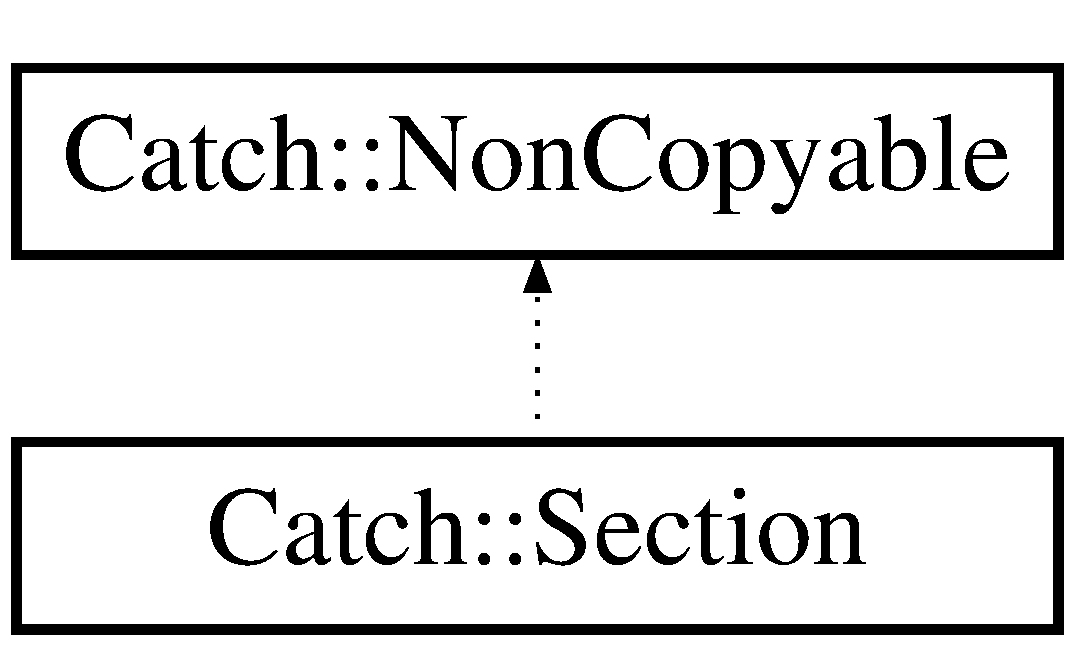
\includegraphics[height=2.000000cm]{classCatch_1_1Section}
\end{center}
\end{figure}
\subsection*{Public Member Functions}
\begin{DoxyCompactItemize}
\item 
{\bfseries Section} (\hyperlink{structCatch_1_1SectionInfo}{Section\+Info} const \&info)\hypertarget{classCatch_1_1Section_a68fd4e51e8981aaa7ddb00d8a6abd099}{}\label{classCatch_1_1Section_a68fd4e51e8981aaa7ddb00d8a6abd099}

\item 
{\bfseries operator bool} () const \hypertarget{classCatch_1_1Section_a6c9be48e8ba0611c4aa601102e706f3b}{}\label{classCatch_1_1Section_a6c9be48e8ba0611c4aa601102e706f3b}

\end{DoxyCompactItemize}


The documentation for this class was generated from the following file\+:\begin{DoxyCompactItemize}
\item 
catch.\+hpp\end{DoxyCompactItemize}

\hypertarget{structCatch_1_1SectionEndInfo}{}\section{Catch\+:\+:Section\+End\+Info Struct Reference}
\label{structCatch_1_1SectionEndInfo}\index{Catch\+::\+Section\+End\+Info@{Catch\+::\+Section\+End\+Info}}
\subsection*{Public Member Functions}
\begin{DoxyCompactItemize}
\item 
{\bfseries Section\+End\+Info} (\hyperlink{structCatch_1_1SectionInfo}{Section\+Info} const \&\+\_\+section\+Info, \hyperlink{structCatch_1_1Counts}{Counts} const \&\+\_\+prev\+Assertions, double \+\_\+duration\+In\+Seconds)\hypertarget{structCatch_1_1SectionEndInfo_abc9381c7c22b6907317ec985ccaa6713}{}\label{structCatch_1_1SectionEndInfo_abc9381c7c22b6907317ec985ccaa6713}

\end{DoxyCompactItemize}
\subsection*{Public Attributes}
\begin{DoxyCompactItemize}
\item 
\hyperlink{structCatch_1_1SectionInfo}{Section\+Info} {\bfseries section\+Info}\hypertarget{structCatch_1_1SectionEndInfo_a2d44793392cb83735d086d726822abe9}{}\label{structCatch_1_1SectionEndInfo_a2d44793392cb83735d086d726822abe9}

\item 
\hyperlink{structCatch_1_1Counts}{Counts} {\bfseries prev\+Assertions}\hypertarget{structCatch_1_1SectionEndInfo_ae70b154cbc05b5dd2901d97f89303d8c}{}\label{structCatch_1_1SectionEndInfo_ae70b154cbc05b5dd2901d97f89303d8c}

\item 
double {\bfseries duration\+In\+Seconds}\hypertarget{structCatch_1_1SectionEndInfo_a7c262f2dab9cff166b8eca620c47eea5}{}\label{structCatch_1_1SectionEndInfo_a7c262f2dab9cff166b8eca620c47eea5}

\end{DoxyCompactItemize}


The documentation for this struct was generated from the following file\+:\begin{DoxyCompactItemize}
\item 
catch.\+hpp\end{DoxyCompactItemize}

\hypertarget{structCatch_1_1SectionInfo}{}\section{Catch\+:\+:Section\+Info Struct Reference}
\label{structCatch_1_1SectionInfo}\index{Catch\+::\+Section\+Info@{Catch\+::\+Section\+Info}}
\subsection*{Public Member Functions}
\begin{DoxyCompactItemize}
\item 
{\bfseries Section\+Info} (\hyperlink{structCatch_1_1SourceLineInfo}{Source\+Line\+Info} const \&\+\_\+line\+Info, std\+::string const \&\+\_\+name, std\+::string const \&\+\_\+description=std\+::string())\hypertarget{structCatch_1_1SectionInfo_a27aff3aaf8b6611f3651b17111a272c6}{}\label{structCatch_1_1SectionInfo_a27aff3aaf8b6611f3651b17111a272c6}

\end{DoxyCompactItemize}
\subsection*{Public Attributes}
\begin{DoxyCompactItemize}
\item 
std\+::string {\bfseries name}\hypertarget{structCatch_1_1SectionInfo_a704c8fc662d309137e0d4f199cb7df58}{}\label{structCatch_1_1SectionInfo_a704c8fc662d309137e0d4f199cb7df58}

\item 
std\+::string {\bfseries description}\hypertarget{structCatch_1_1SectionInfo_a0052060219a6de74bb7ade34d4163a4e}{}\label{structCatch_1_1SectionInfo_a0052060219a6de74bb7ade34d4163a4e}

\item 
\hyperlink{structCatch_1_1SourceLineInfo}{Source\+Line\+Info} {\bfseries line\+Info}\hypertarget{structCatch_1_1SectionInfo_adbc83b8a3507c4acc8ee249e93465711}{}\label{structCatch_1_1SectionInfo_adbc83b8a3507c4acc8ee249e93465711}

\end{DoxyCompactItemize}


The documentation for this struct was generated from the following file\+:\begin{DoxyCompactItemize}
\item 
catch.\+hpp\end{DoxyCompactItemize}

\hypertarget{structCatch_1_1SharedImpl}{}\section{Catch\+:\+:Shared\+Impl$<$ T $>$ Struct Template Reference}
\label{structCatch_1_1SharedImpl}\index{Catch\+::\+Shared\+Impl$<$ T $>$@{Catch\+::\+Shared\+Impl$<$ T $>$}}
Inheritance diagram for Catch\+:\+:Shared\+Impl$<$ T $>$\+:\begin{figure}[H]
\begin{center}
\leavevmode
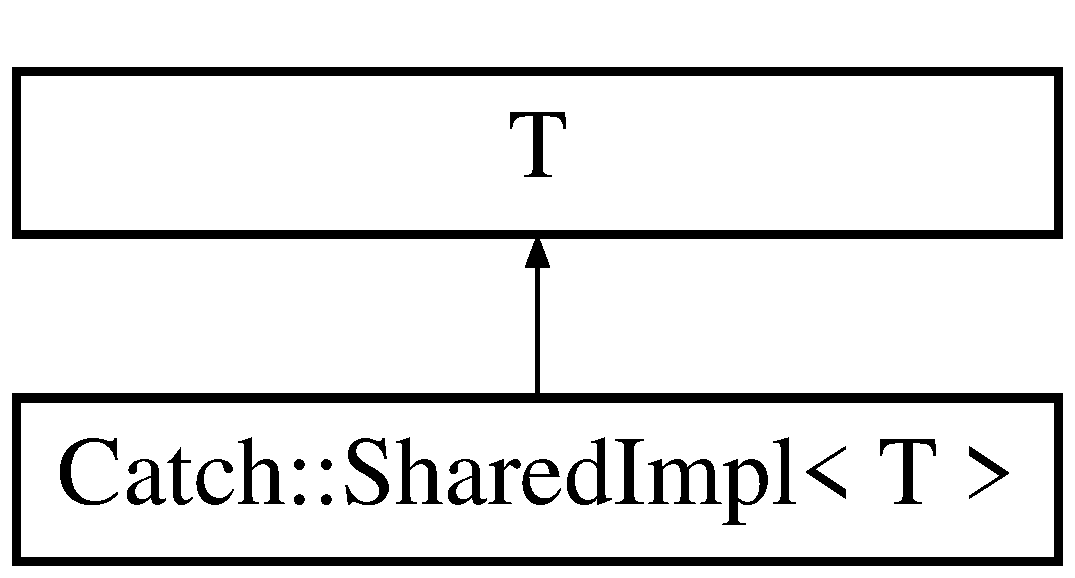
\includegraphics[height=2.000000cm]{structCatch_1_1SharedImpl}
\end{center}
\end{figure}
\subsection*{Public Member Functions}
\begin{DoxyCompactItemize}
\item 
virtual void {\bfseries add\+Ref} () const \hypertarget{structCatch_1_1SharedImpl_a9b190b7a139a09d2624d1201d8e4f87e}{}\label{structCatch_1_1SharedImpl_a9b190b7a139a09d2624d1201d8e4f87e}

\item 
virtual void {\bfseries release} () const \hypertarget{structCatch_1_1SharedImpl_a16baad80ad5ad3dfaf2a10a157a02e01}{}\label{structCatch_1_1SharedImpl_a16baad80ad5ad3dfaf2a10a157a02e01}

\end{DoxyCompactItemize}
\subsection*{Public Attributes}
\begin{DoxyCompactItemize}
\item 
unsigned int {\bfseries m\+\_\+rc}\hypertarget{structCatch_1_1SharedImpl_a7e71ef1985b85aa41a1632f932a96bcb}{}\label{structCatch_1_1SharedImpl_a7e71ef1985b85aa41a1632f932a96bcb}

\end{DoxyCompactItemize}


The documentation for this struct was generated from the following file\+:\begin{DoxyCompactItemize}
\item 
catch.\+hpp\end{DoxyCompactItemize}

\hypertarget{structCatch_1_1SourceLineInfo}{}\section{Catch\+:\+:Source\+Line\+Info Struct Reference}
\label{structCatch_1_1SourceLineInfo}\index{Catch\+::\+Source\+Line\+Info@{Catch\+::\+Source\+Line\+Info}}
\subsection*{Public Member Functions}
\begin{DoxyCompactItemize}
\item 
{\bfseries Source\+Line\+Info} (char const $\ast$\+\_\+file, std\+::size\+\_\+t \+\_\+line)\hypertarget{structCatch_1_1SourceLineInfo_a6218cb890337d37f708ea94063958940}{}\label{structCatch_1_1SourceLineInfo_a6218cb890337d37f708ea94063958940}

\item 
{\bfseries Source\+Line\+Info} (\hyperlink{structCatch_1_1SourceLineInfo}{Source\+Line\+Info} const \&other)\hypertarget{structCatch_1_1SourceLineInfo_a1ec99cc0547ce5909133aaa8f14ed4b1}{}\label{structCatch_1_1SourceLineInfo_a1ec99cc0547ce5909133aaa8f14ed4b1}

\item 
bool {\bfseries empty} () const \hypertarget{structCatch_1_1SourceLineInfo_a9a25ffc0640d1a3dd0c9b7e5fcbba7b9}{}\label{structCatch_1_1SourceLineInfo_a9a25ffc0640d1a3dd0c9b7e5fcbba7b9}

\item 
bool {\bfseries operator==} (\hyperlink{structCatch_1_1SourceLineInfo}{Source\+Line\+Info} const \&other) const \hypertarget{structCatch_1_1SourceLineInfo_af0854821b1abfda52796ef0f1294b050}{}\label{structCatch_1_1SourceLineInfo_af0854821b1abfda52796ef0f1294b050}

\item 
bool {\bfseries operator$<$} (\hyperlink{structCatch_1_1SourceLineInfo}{Source\+Line\+Info} const \&other) const \hypertarget{structCatch_1_1SourceLineInfo_a581c02d683808232168bfc2e775c3554}{}\label{structCatch_1_1SourceLineInfo_a581c02d683808232168bfc2e775c3554}

\end{DoxyCompactItemize}
\subsection*{Public Attributes}
\begin{DoxyCompactItemize}
\item 
std\+::string {\bfseries file}\hypertarget{structCatch_1_1SourceLineInfo_adf3ccf0c2bd326eb3466318af82a94dd}{}\label{structCatch_1_1SourceLineInfo_adf3ccf0c2bd326eb3466318af82a94dd}

\item 
std\+::size\+\_\+t {\bfseries line}\hypertarget{structCatch_1_1SourceLineInfo_a841e5d696c7b9cde24e45e61dd979c77}{}\label{structCatch_1_1SourceLineInfo_a841e5d696c7b9cde24e45e61dd979c77}

\end{DoxyCompactItemize}


The documentation for this struct was generated from the following file\+:\begin{DoxyCompactItemize}
\item 
catch.\+hpp\end{DoxyCompactItemize}

\hypertarget{structCatch_1_1Matchers_1_1Impl_1_1StdString_1_1StartsWith}{}\section{Catch\+:\+:Matchers\+:\+:Impl\+:\+:Std\+String\+:\+:Starts\+With Struct Reference}
\label{structCatch_1_1Matchers_1_1Impl_1_1StdString_1_1StartsWith}\index{Catch\+::\+Matchers\+::\+Impl\+::\+Std\+String\+::\+Starts\+With@{Catch\+::\+Matchers\+::\+Impl\+::\+Std\+String\+::\+Starts\+With}}
Inheritance diagram for Catch\+:\+:Matchers\+:\+:Impl\+:\+:Std\+String\+:\+:Starts\+With\+:\begin{figure}[H]
\begin{center}
\leavevmode
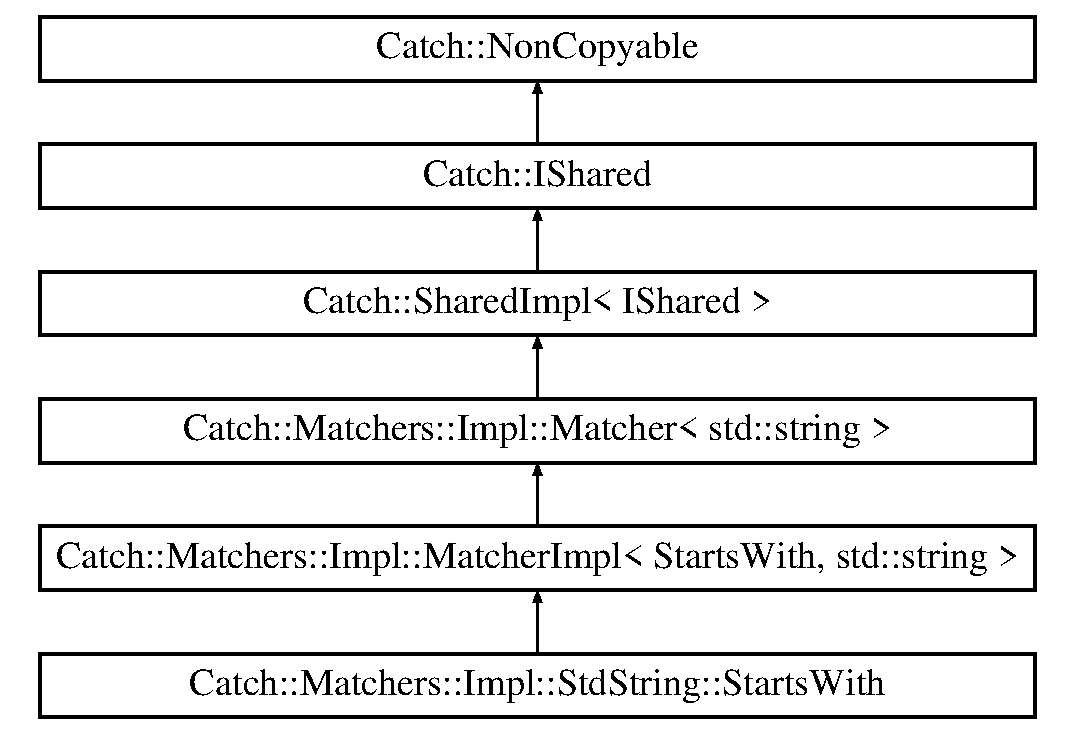
\includegraphics[height=6.000000cm]{structCatch_1_1Matchers_1_1Impl_1_1StdString_1_1StartsWith}
\end{center}
\end{figure}
\subsection*{Public Member Functions}
\begin{DoxyCompactItemize}
\item 
{\bfseries Starts\+With} (std\+::string const \&substr, Case\+Sensitive\+::\+Choice case\+Sensitivity=Case\+Sensitive\+::\+Yes)\hypertarget{structCatch_1_1Matchers_1_1Impl_1_1StdString_1_1StartsWith_a0db1bd8876219464ae60346c9525bcf6}{}\label{structCatch_1_1Matchers_1_1Impl_1_1StdString_1_1StartsWith_a0db1bd8876219464ae60346c9525bcf6}

\item 
{\bfseries Starts\+With} (\hyperlink{structCatch_1_1Matchers_1_1Impl_1_1StdString_1_1StartsWith}{Starts\+With} const \&other)\hypertarget{structCatch_1_1Matchers_1_1Impl_1_1StdString_1_1StartsWith_a5526cb587632e7e46253d6f60ae01098}{}\label{structCatch_1_1Matchers_1_1Impl_1_1StdString_1_1StartsWith_a5526cb587632e7e46253d6f60ae01098}

\item 
virtual bool {\bfseries match} (std\+::string const \&expr) const \hypertarget{structCatch_1_1Matchers_1_1Impl_1_1StdString_1_1StartsWith_ae9c893adbacc853171a488aea5355653}{}\label{structCatch_1_1Matchers_1_1Impl_1_1StdString_1_1StartsWith_ae9c893adbacc853171a488aea5355653}

\item 
virtual std\+::string {\bfseries to\+String} () const \hypertarget{structCatch_1_1Matchers_1_1Impl_1_1StdString_1_1StartsWith_a066fe10e74495cb556abc6895193ba97}{}\label{structCatch_1_1Matchers_1_1Impl_1_1StdString_1_1StartsWith_a066fe10e74495cb556abc6895193ba97}

\end{DoxyCompactItemize}
\subsection*{Public Attributes}
\begin{DoxyCompactItemize}
\item 
\hyperlink{structCatch_1_1Matchers_1_1Impl_1_1StdString_1_1CasedString}{Cased\+String} {\bfseries m\+\_\+data}\hypertarget{structCatch_1_1Matchers_1_1Impl_1_1StdString_1_1StartsWith_accaace83106244c635d251addb028125}{}\label{structCatch_1_1Matchers_1_1Impl_1_1StdString_1_1StartsWith_accaace83106244c635d251addb028125}

\end{DoxyCompactItemize}
\subsection*{Additional Inherited Members}


The documentation for this struct was generated from the following file\+:\begin{DoxyCompactItemize}
\item 
catch.\+hpp\end{DoxyCompactItemize}

\hypertarget{structCatch_1_1StreamEndStop}{}\section{Catch\+:\+:Stream\+End\+Stop Struct Reference}
\label{structCatch_1_1StreamEndStop}\index{Catch\+::\+Stream\+End\+Stop@{Catch\+::\+Stream\+End\+Stop}}
\subsection*{Public Member Functions}
\begin{DoxyCompactItemize}
\item 
std\+::string {\bfseries operator+} ()\hypertarget{structCatch_1_1StreamEndStop_a3025092e06c224e0845f2caa07b26d0e}{}\label{structCatch_1_1StreamEndStop_a3025092e06c224e0845f2caa07b26d0e}

\end{DoxyCompactItemize}


The documentation for this struct was generated from the following file\+:\begin{DoxyCompactItemize}
\item 
catch.\+hpp\end{DoxyCompactItemize}

\hypertarget{structCatch_1_1StringMaker}{}\section{Catch\+:\+:String\+Maker$<$ T $>$ Struct Template Reference}
\label{structCatch_1_1StringMaker}\index{Catch\+::\+String\+Maker$<$ T $>$@{Catch\+::\+String\+Maker$<$ T $>$}}
Inheritance diagram for Catch\+:\+:String\+Maker$<$ T $>$\+:\begin{figure}[H]
\begin{center}
\leavevmode
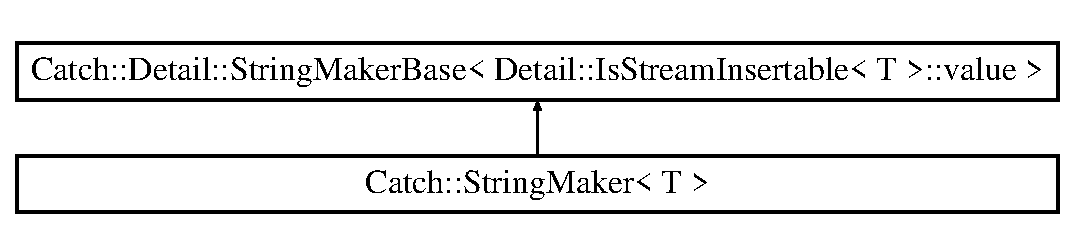
\includegraphics[height=2.000000cm]{structCatch_1_1StringMaker}
\end{center}
\end{figure}
\subsection*{Additional Inherited Members}


The documentation for this struct was generated from the following file\+:\begin{DoxyCompactItemize}
\item 
catch.\+hpp\end{DoxyCompactItemize}

\hypertarget{structCatch_1_1StringMaker_3_01R_01C_1_1_5_01_4}{}\section{Catch\+:\+:String\+Maker$<$ R C\+:\+:$\ast$ $>$ Struct Template Reference}
\label{structCatch_1_1StringMaker_3_01R_01C_1_1_5_01_4}\index{Catch\+::\+String\+Maker$<$ R C\+::$\ast$ $>$@{Catch\+::\+String\+Maker$<$ R C\+::$\ast$ $>$}}
\subsection*{Static Public Member Functions}
\begin{DoxyCompactItemize}
\item 
static std\+::string {\bfseries convert} (R C\+::$\ast$p)\hypertarget{structCatch_1_1StringMaker_3_01R_01C_1_1_5_01_4_af69c15e0b406e945777137fe4a333731}{}\label{structCatch_1_1StringMaker_3_01R_01C_1_1_5_01_4_af69c15e0b406e945777137fe4a333731}

\end{DoxyCompactItemize}


The documentation for this struct was generated from the following file\+:\begin{DoxyCompactItemize}
\item 
catch.\+hpp\end{DoxyCompactItemize}

\hypertarget{structCatch_1_1StringMaker_3_01T_01_5_01_4}{}\section{Catch\+:\+:String\+Maker$<$ T $\ast$ $>$ Struct Template Reference}
\label{structCatch_1_1StringMaker_3_01T_01_5_01_4}\index{Catch\+::\+String\+Maker$<$ T $\ast$ $>$@{Catch\+::\+String\+Maker$<$ T $\ast$ $>$}}
\subsection*{Static Public Member Functions}
\begin{DoxyCompactItemize}
\item 
{\footnotesize template$<$typename U $>$ }\\static std\+::string {\bfseries convert} (U $\ast$p)\hypertarget{structCatch_1_1StringMaker_3_01T_01_5_01_4_a2adbc75c99d71b8323f4052bcb0815c9}{}\label{structCatch_1_1StringMaker_3_01T_01_5_01_4_a2adbc75c99d71b8323f4052bcb0815c9}

\end{DoxyCompactItemize}


The documentation for this struct was generated from the following file\+:\begin{DoxyCompactItemize}
\item 
catch.\+hpp\end{DoxyCompactItemize}

\hypertarget{structCatch_1_1Detail_1_1StringMakerBase}{}\section{Catch\+:\+:Detail\+:\+:String\+Maker\+Base$<$ C $>$ Struct Template Reference}
\label{structCatch_1_1Detail_1_1StringMakerBase}\index{Catch\+::\+Detail\+::\+String\+Maker\+Base$<$ C $>$@{Catch\+::\+Detail\+::\+String\+Maker\+Base$<$ C $>$}}
\subsection*{Static Public Member Functions}
\begin{DoxyCompactItemize}
\item 
{\footnotesize template$<$typename T $>$ }\\static std\+::string {\bfseries convert} (T const \&)\hypertarget{structCatch_1_1Detail_1_1StringMakerBase_a8eb9f635dc413a5758e22614bafaf1a3}{}\label{structCatch_1_1Detail_1_1StringMakerBase_a8eb9f635dc413a5758e22614bafaf1a3}

\end{DoxyCompactItemize}


The documentation for this struct was generated from the following file\+:\begin{DoxyCompactItemize}
\item 
catch.\+hpp\end{DoxyCompactItemize}

\hypertarget{structCatch_1_1Detail_1_1StringMakerBase_3_01true_01_4}{}\section{Catch\+:\+:Detail\+:\+:String\+Maker\+Base$<$ true $>$ Struct Template Reference}
\label{structCatch_1_1Detail_1_1StringMakerBase_3_01true_01_4}\index{Catch\+::\+Detail\+::\+String\+Maker\+Base$<$ true $>$@{Catch\+::\+Detail\+::\+String\+Maker\+Base$<$ true $>$}}
\subsection*{Static Public Member Functions}
\begin{DoxyCompactItemize}
\item 
{\footnotesize template$<$typename T $>$ }\\static std\+::string {\bfseries convert} (T const \&\+\_\+value)\hypertarget{structCatch_1_1Detail_1_1StringMakerBase_3_01true_01_4_af9b5fdf7fddd8c5c873caa819e5f00f6}{}\label{structCatch_1_1Detail_1_1StringMakerBase_3_01true_01_4_af9b5fdf7fddd8c5c873caa819e5f00f6}

\end{DoxyCompactItemize}


The documentation for this struct was generated from the following file\+:\begin{DoxyCompactItemize}
\item 
catch.\+hpp\end{DoxyCompactItemize}

\hypertarget{structCatch_1_1TagAlias}{}\section{Catch\+:\+:Tag\+Alias Struct Reference}
\label{structCatch_1_1TagAlias}\index{Catch\+::\+Tag\+Alias@{Catch\+::\+Tag\+Alias}}
\subsection*{Public Member Functions}
\begin{DoxyCompactItemize}
\item 
{\bfseries Tag\+Alias} (std\+::string \+\_\+tag, \hyperlink{structCatch_1_1SourceLineInfo}{Source\+Line\+Info} \+\_\+line\+Info)\hypertarget{structCatch_1_1TagAlias_ad9124d03bfb6f767f1c97572330b05bc}{}\label{structCatch_1_1TagAlias_ad9124d03bfb6f767f1c97572330b05bc}

\end{DoxyCompactItemize}
\subsection*{Public Attributes}
\begin{DoxyCompactItemize}
\item 
std\+::string {\bfseries tag}\hypertarget{structCatch_1_1TagAlias_a950183883ab17c90d0fab16b966b6e2d}{}\label{structCatch_1_1TagAlias_a950183883ab17c90d0fab16b966b6e2d}

\item 
\hyperlink{structCatch_1_1SourceLineInfo}{Source\+Line\+Info} {\bfseries line\+Info}\hypertarget{structCatch_1_1TagAlias_a2f51fe0b3c052561275d26b6eb88f702}{}\label{structCatch_1_1TagAlias_a2f51fe0b3c052561275d26b6eb88f702}

\end{DoxyCompactItemize}


The documentation for this struct was generated from the following file\+:\begin{DoxyCompactItemize}
\item 
catch.\+hpp\end{DoxyCompactItemize}

\hypertarget{classCatch_1_1TestCase}{}\section{Catch\+:\+:Test\+Case Class Reference}
\label{classCatch_1_1TestCase}\index{Catch\+::\+Test\+Case@{Catch\+::\+Test\+Case}}
Inheritance diagram for Catch\+:\+:Test\+Case\+:\begin{figure}[H]
\begin{center}
\leavevmode
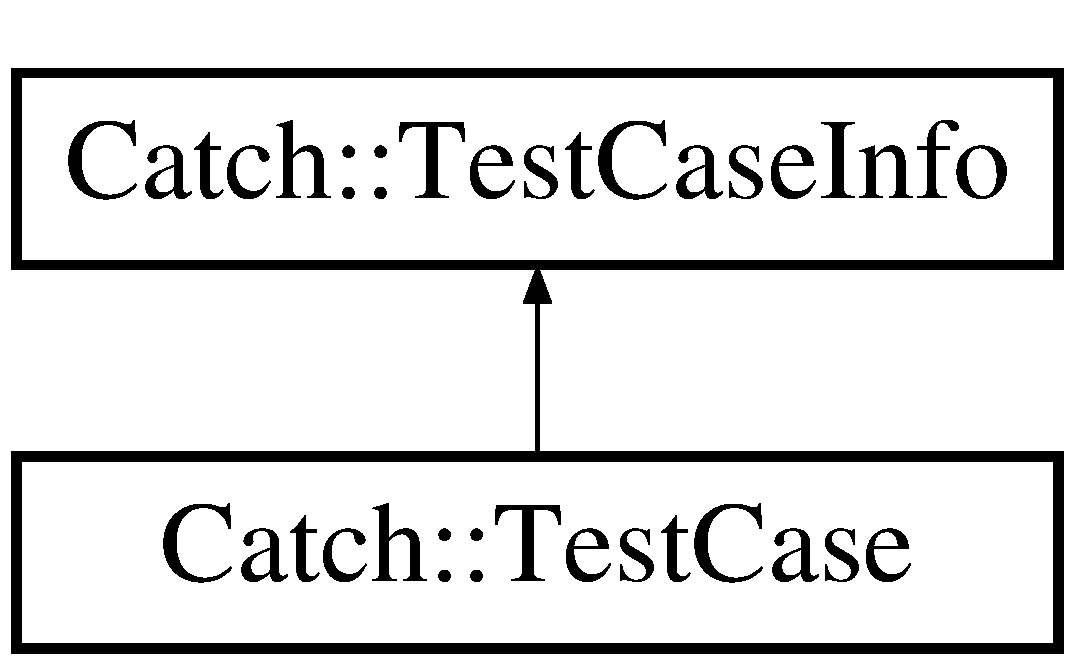
\includegraphics[height=2.000000cm]{classCatch_1_1TestCase}
\end{center}
\end{figure}
\subsection*{Public Member Functions}
\begin{DoxyCompactItemize}
\item 
{\bfseries Test\+Case} (\hyperlink{structCatch_1_1ITestCase}{I\+Test\+Case} $\ast$test\+Case, \hyperlink{structCatch_1_1TestCaseInfo}{Test\+Case\+Info} const \&info)\hypertarget{classCatch_1_1TestCase_a03a5b913484681bd6d398dc5e9c2a907}{}\label{classCatch_1_1TestCase_a03a5b913484681bd6d398dc5e9c2a907}

\item 
{\bfseries Test\+Case} (\hyperlink{classCatch_1_1TestCase}{Test\+Case} const \&other)\hypertarget{classCatch_1_1TestCase_ac0011d3789edc3e44edb41f13c4775a0}{}\label{classCatch_1_1TestCase_ac0011d3789edc3e44edb41f13c4775a0}

\item 
\hyperlink{classCatch_1_1TestCase}{Test\+Case} {\bfseries with\+Name} (std\+::string const \&\+\_\+new\+Name) const \hypertarget{classCatch_1_1TestCase_ab6dbc6c82b7c1680013c67bdedccfc8e}{}\label{classCatch_1_1TestCase_ab6dbc6c82b7c1680013c67bdedccfc8e}

\item 
void {\bfseries invoke} () const \hypertarget{classCatch_1_1TestCase_aac2e028135cc88c3e3aac04650960a6c}{}\label{classCatch_1_1TestCase_aac2e028135cc88c3e3aac04650960a6c}

\item 
\hyperlink{structCatch_1_1TestCaseInfo}{Test\+Case\+Info} const \& {\bfseries get\+Test\+Case\+Info} () const \hypertarget{classCatch_1_1TestCase_a25c03661ab092431cdff10df5c58a5a7}{}\label{classCatch_1_1TestCase_a25c03661ab092431cdff10df5c58a5a7}

\item 
void {\bfseries swap} (\hyperlink{classCatch_1_1TestCase}{Test\+Case} \&other)\hypertarget{classCatch_1_1TestCase_aee38f908faf10b905b209ca388275413}{}\label{classCatch_1_1TestCase_aee38f908faf10b905b209ca388275413}

\item 
bool {\bfseries operator==} (\hyperlink{classCatch_1_1TestCase}{Test\+Case} const \&other) const \hypertarget{classCatch_1_1TestCase_a40eab521b316c7d476f6b4dd1c33eec8}{}\label{classCatch_1_1TestCase_a40eab521b316c7d476f6b4dd1c33eec8}

\item 
bool {\bfseries operator$<$} (\hyperlink{classCatch_1_1TestCase}{Test\+Case} const \&other) const \hypertarget{classCatch_1_1TestCase_aa5174e85e3aac6e7398dee9c76730324}{}\label{classCatch_1_1TestCase_aa5174e85e3aac6e7398dee9c76730324}

\item 
\hyperlink{classCatch_1_1TestCase}{Test\+Case} \& {\bfseries operator=} (\hyperlink{classCatch_1_1TestCase}{Test\+Case} const \&other)\hypertarget{classCatch_1_1TestCase_a8022e3f74232f7887d2d2cbbc8876502}{}\label{classCatch_1_1TestCase_a8022e3f74232f7887d2d2cbbc8876502}

\end{DoxyCompactItemize}
\subsection*{Additional Inherited Members}


The documentation for this class was generated from the following file\+:\begin{DoxyCompactItemize}
\item 
catch.\+hpp\end{DoxyCompactItemize}

\hypertarget{structCatch_1_1TestCaseInfo}{}\section{Catch\+:\+:Test\+Case\+Info Struct Reference}
\label{structCatch_1_1TestCaseInfo}\index{Catch\+::\+Test\+Case\+Info@{Catch\+::\+Test\+Case\+Info}}
Inheritance diagram for Catch\+:\+:Test\+Case\+Info\+:\begin{figure}[H]
\begin{center}
\leavevmode
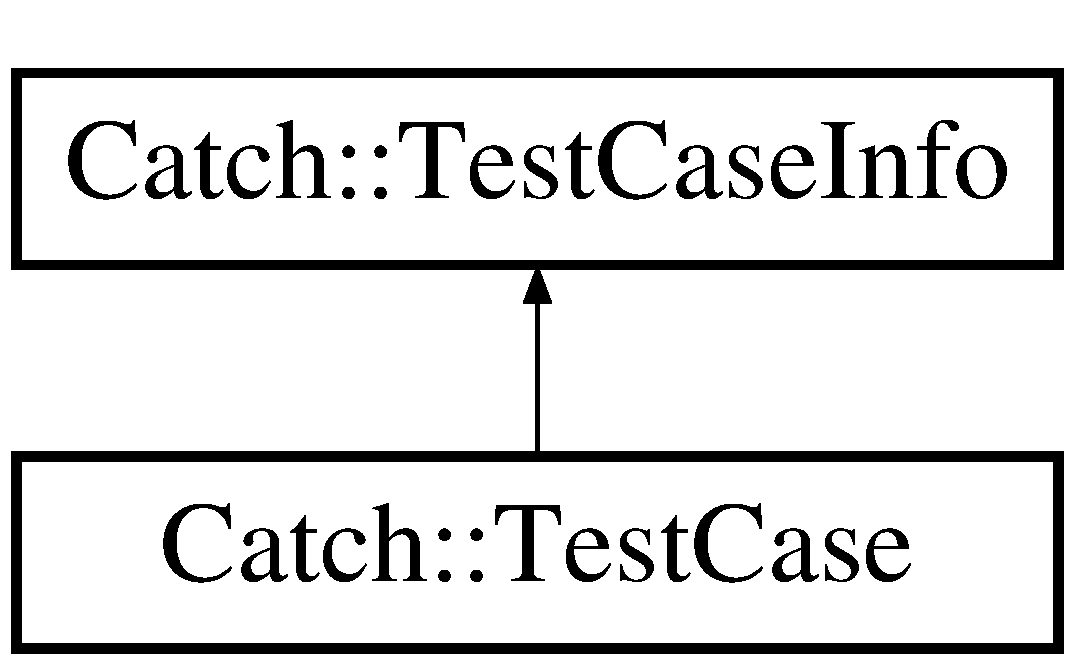
\includegraphics[height=2.000000cm]{structCatch_1_1TestCaseInfo}
\end{center}
\end{figure}
\subsection*{Public Types}
\begin{DoxyCompactItemize}
\item 
enum {\bfseries Special\+Properties} \{ \\*
{\bfseries None} = 0, 
{\bfseries Is\+Hidden} = 1 $<$$<$ 1, 
{\bfseries Should\+Fail} = 1 $<$$<$ 2, 
{\bfseries May\+Fail} = 1 $<$$<$ 3, 
\\*
{\bfseries Throws} = 1 $<$$<$ 4
 \}\hypertarget{structCatch_1_1TestCaseInfo_a39b232f74b4a7a6f2183b96759027eac}{}\label{structCatch_1_1TestCaseInfo_a39b232f74b4a7a6f2183b96759027eac}

\end{DoxyCompactItemize}
\subsection*{Public Member Functions}
\begin{DoxyCompactItemize}
\item 
{\bfseries Test\+Case\+Info} (std\+::string const \&\+\_\+name, std\+::string const \&\+\_\+class\+Name, std\+::string const \&\+\_\+description, std\+::set$<$ std\+::string $>$ const \&\+\_\+tags, \hyperlink{structCatch_1_1SourceLineInfo}{Source\+Line\+Info} const \&\+\_\+line\+Info)\hypertarget{structCatch_1_1TestCaseInfo_a35ec65315e0d1f178491b5a59f3f3123}{}\label{structCatch_1_1TestCaseInfo_a35ec65315e0d1f178491b5a59f3f3123}

\item 
{\bfseries Test\+Case\+Info} (\hyperlink{structCatch_1_1TestCaseInfo}{Test\+Case\+Info} const \&other)\hypertarget{structCatch_1_1TestCaseInfo_ac338adb4e38f4bf3977fb45b2b1fe447}{}\label{structCatch_1_1TestCaseInfo_ac338adb4e38f4bf3977fb45b2b1fe447}

\item 
bool {\bfseries is\+Hidden} () const \hypertarget{structCatch_1_1TestCaseInfo_a01ac8b11d8c105e5278a239ab5214257}{}\label{structCatch_1_1TestCaseInfo_a01ac8b11d8c105e5278a239ab5214257}

\item 
bool {\bfseries throws} () const \hypertarget{structCatch_1_1TestCaseInfo_a19fb4f0b755956eee8a1fecf713fb7ca}{}\label{structCatch_1_1TestCaseInfo_a19fb4f0b755956eee8a1fecf713fb7ca}

\item 
bool {\bfseries ok\+To\+Fail} () const \hypertarget{structCatch_1_1TestCaseInfo_a64586336bb49bd6e9ef8a089b072a712}{}\label{structCatch_1_1TestCaseInfo_a64586336bb49bd6e9ef8a089b072a712}

\item 
bool {\bfseries expected\+To\+Fail} () const \hypertarget{structCatch_1_1TestCaseInfo_a1ed1c3689c2874c421466945bd3cb75c}{}\label{structCatch_1_1TestCaseInfo_a1ed1c3689c2874c421466945bd3cb75c}

\end{DoxyCompactItemize}
\subsection*{Public Attributes}
\begin{DoxyCompactItemize}
\item 
std\+::string {\bfseries name}\hypertarget{structCatch_1_1TestCaseInfo_a463794e2f5cfead307c93efd134ade36}{}\label{structCatch_1_1TestCaseInfo_a463794e2f5cfead307c93efd134ade36}

\item 
std\+::string {\bfseries class\+Name}\hypertarget{structCatch_1_1TestCaseInfo_a1a5e0825132a38d091defdebbf2f8ce9}{}\label{structCatch_1_1TestCaseInfo_a1a5e0825132a38d091defdebbf2f8ce9}

\item 
std\+::string {\bfseries description}\hypertarget{structCatch_1_1TestCaseInfo_a37fe2db9425bc45f6a33893eac31198e}{}\label{structCatch_1_1TestCaseInfo_a37fe2db9425bc45f6a33893eac31198e}

\item 
std\+::set$<$ std\+::string $>$ {\bfseries tags}\hypertarget{structCatch_1_1TestCaseInfo_a045f62e7719a8760a5b456f7fd2dc97c}{}\label{structCatch_1_1TestCaseInfo_a045f62e7719a8760a5b456f7fd2dc97c}

\item 
std\+::set$<$ std\+::string $>$ {\bfseries lcase\+Tags}\hypertarget{structCatch_1_1TestCaseInfo_a0ed3864a313e8ddc3ae38431be5be9ae}{}\label{structCatch_1_1TestCaseInfo_a0ed3864a313e8ddc3ae38431be5be9ae}

\item 
std\+::string {\bfseries tags\+As\+String}\hypertarget{structCatch_1_1TestCaseInfo_ac65c2d36fd36f71e9bf782b2ea245c64}{}\label{structCatch_1_1TestCaseInfo_ac65c2d36fd36f71e9bf782b2ea245c64}

\item 
\hyperlink{structCatch_1_1SourceLineInfo}{Source\+Line\+Info} {\bfseries line\+Info}\hypertarget{structCatch_1_1TestCaseInfo_aa9407b7f442655b51a2aad24b3fa2fd3}{}\label{structCatch_1_1TestCaseInfo_aa9407b7f442655b51a2aad24b3fa2fd3}

\item 
Special\+Properties {\bfseries properties}\hypertarget{structCatch_1_1TestCaseInfo_afc1e84bd7a2e180895a06d9131302af0}{}\label{structCatch_1_1TestCaseInfo_afc1e84bd7a2e180895a06d9131302af0}

\end{DoxyCompactItemize}
\subsection*{Friends}
\begin{DoxyCompactItemize}
\item 
void {\bfseries set\+Tags} (\hyperlink{structCatch_1_1TestCaseInfo}{Test\+Case\+Info} \&test\+Case\+Info, std\+::set$<$ std\+::string $>$ const \&tags)\hypertarget{structCatch_1_1TestCaseInfo_addc10c770e56f49da5baa0c76cf25bd5}{}\label{structCatch_1_1TestCaseInfo_addc10c770e56f49da5baa0c76cf25bd5}

\end{DoxyCompactItemize}


The documentation for this struct was generated from the following file\+:\begin{DoxyCompactItemize}
\item 
catch.\+hpp\end{DoxyCompactItemize}

\hypertarget{structCatch_1_1TestFailureException}{}\section{Catch\+:\+:Test\+Failure\+Exception Struct Reference}
\label{structCatch_1_1TestFailureException}\index{Catch\+::\+Test\+Failure\+Exception@{Catch\+::\+Test\+Failure\+Exception}}


The documentation for this struct was generated from the following file\+:\begin{DoxyCompactItemize}
\item 
catch.\+hpp\end{DoxyCompactItemize}

\hypertarget{classCatch_1_1Timer}{}\section{Catch\+:\+:Timer Class Reference}
\label{classCatch_1_1Timer}\index{Catch\+::\+Timer@{Catch\+::\+Timer}}
\subsection*{Public Member Functions}
\begin{DoxyCompactItemize}
\item 
void {\bfseries start} ()\hypertarget{classCatch_1_1Timer_a0a56e879e43f36c102bf9ea8b5fc8b72}{}\label{classCatch_1_1Timer_a0a56e879e43f36c102bf9ea8b5fc8b72}

\item 
unsigned int {\bfseries get\+Elapsed\+Microseconds} () const \hypertarget{classCatch_1_1Timer_a4b0062f169f7d3150b0e8073ab37890a}{}\label{classCatch_1_1Timer_a4b0062f169f7d3150b0e8073ab37890a}

\item 
unsigned int {\bfseries get\+Elapsed\+Milliseconds} () const \hypertarget{classCatch_1_1Timer_a4cf3f9fbee9c76e87d989d9bc6913b68}{}\label{classCatch_1_1Timer_a4cf3f9fbee9c76e87d989d9bc6913b68}

\item 
double {\bfseries get\+Elapsed\+Seconds} () const \hypertarget{classCatch_1_1Timer_a8500ef3481a9bf6ae81337972d9f95a3}{}\label{classCatch_1_1Timer_a8500ef3481a9bf6ae81337972d9f95a3}

\end{DoxyCompactItemize}


The documentation for this class was generated from the following file\+:\begin{DoxyCompactItemize}
\item 
catch.\+hpp\end{DoxyCompactItemize}

\hypertarget{structCatch_1_1Totals}{}\section{Catch\+:\+:Totals Struct Reference}
\label{structCatch_1_1Totals}\index{Catch\+::\+Totals@{Catch\+::\+Totals}}
\subsection*{Public Member Functions}
\begin{DoxyCompactItemize}
\item 
\hyperlink{structCatch_1_1Totals}{Totals} {\bfseries operator-\/} (\hyperlink{structCatch_1_1Totals}{Totals} const \&other) const \hypertarget{structCatch_1_1Totals_abe15cd8a82ba9a4868dd7a542add827c}{}\label{structCatch_1_1Totals_abe15cd8a82ba9a4868dd7a542add827c}

\item 
\hyperlink{structCatch_1_1Totals}{Totals} {\bfseries delta} (\hyperlink{structCatch_1_1Totals}{Totals} const \&prev\+Totals) const \hypertarget{structCatch_1_1Totals_a3dee0f599c081a8360c0112fb1dafe8f}{}\label{structCatch_1_1Totals_a3dee0f599c081a8360c0112fb1dafe8f}

\item 
\hyperlink{structCatch_1_1Totals}{Totals} \& {\bfseries operator+=} (\hyperlink{structCatch_1_1Totals}{Totals} const \&other)\hypertarget{structCatch_1_1Totals_a574015076e54cc405c70b053e3356e43}{}\label{structCatch_1_1Totals_a574015076e54cc405c70b053e3356e43}

\end{DoxyCompactItemize}
\subsection*{Public Attributes}
\begin{DoxyCompactItemize}
\item 
\hyperlink{structCatch_1_1Counts}{Counts} {\bfseries assertions}\hypertarget{structCatch_1_1Totals_a885ded66df752147b30c3d45aa602ec9}{}\label{structCatch_1_1Totals_a885ded66df752147b30c3d45aa602ec9}

\item 
\hyperlink{structCatch_1_1Counts}{Counts} {\bfseries test\+Cases}\hypertarget{structCatch_1_1Totals_adb195fe477aedee2ecea88c888f16506}{}\label{structCatch_1_1Totals_adb195fe477aedee2ecea88c888f16506}

\end{DoxyCompactItemize}


The documentation for this struct was generated from the following file\+:\begin{DoxyCompactItemize}
\item 
catch.\+hpp\end{DoxyCompactItemize}

\hypertarget{structCatch_1_1Detail_1_1TrueType}{}\section{Catch\+:\+:Detail\+:\+:True\+Type Struct Reference}
\label{structCatch_1_1Detail_1_1TrueType}\index{Catch\+::\+Detail\+::\+True\+Type@{Catch\+::\+Detail\+::\+True\+Type}}
\subsection*{Public Attributes}
\begin{DoxyCompactItemize}
\item 
char {\bfseries sizer} \mbox{[}1\mbox{]}\hypertarget{structCatch_1_1Detail_1_1TrueType_a3aaaeb75909e668b293c8a81f5fb6419}{}\label{structCatch_1_1Detail_1_1TrueType_a3aaaeb75909e668b293c8a81f5fb6419}

\end{DoxyCompactItemize}


The documentation for this struct was generated from the following file\+:\begin{DoxyCompactItemize}
\item 
catch.\+hpp\end{DoxyCompactItemize}

\hypertarget{classCatch_1_1ValuesGenerator}{}\section{Catch\+:\+:Values\+Generator$<$ T $>$ Class Template Reference}
\label{classCatch_1_1ValuesGenerator}\index{Catch\+::\+Values\+Generator$<$ T $>$@{Catch\+::\+Values\+Generator$<$ T $>$}}
Inheritance diagram for Catch\+:\+:Values\+Generator$<$ T $>$\+:\begin{figure}[H]
\begin{center}
\leavevmode
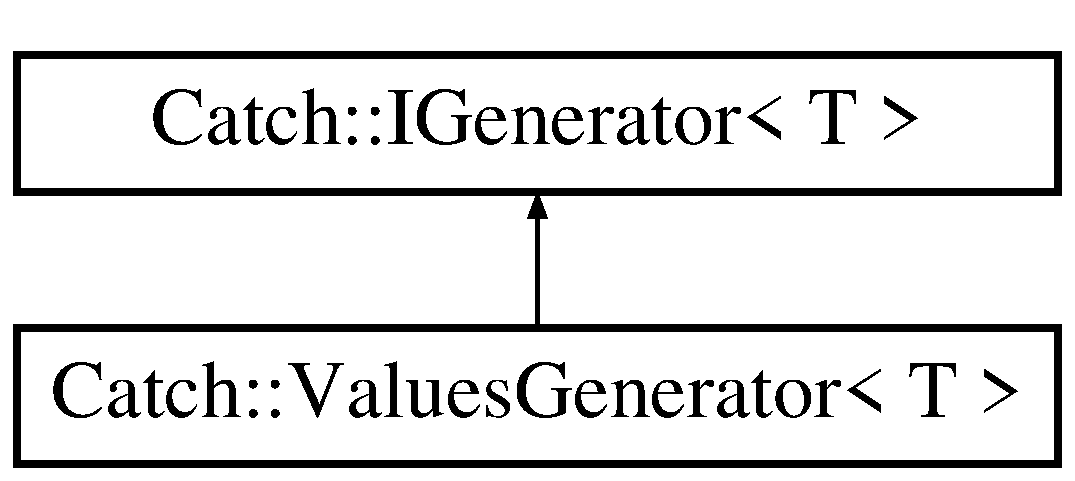
\includegraphics[height=2.000000cm]{classCatch_1_1ValuesGenerator}
\end{center}
\end{figure}
\subsection*{Public Member Functions}
\begin{DoxyCompactItemize}
\item 
void {\bfseries add} (T value)\hypertarget{classCatch_1_1ValuesGenerator_a8412c8ce5d9d4fc6ff06d5246d56d538}{}\label{classCatch_1_1ValuesGenerator_a8412c8ce5d9d4fc6ff06d5246d56d538}

\item 
virtual T {\bfseries get\+Value} (std\+::size\+\_\+t index) const \hypertarget{classCatch_1_1ValuesGenerator_a60599dd67096ff108471f64ee42acd9d}{}\label{classCatch_1_1ValuesGenerator_a60599dd67096ff108471f64ee42acd9d}

\item 
virtual std\+::size\+\_\+t {\bfseries size} () const \hypertarget{classCatch_1_1ValuesGenerator_a98a80bb0dd682c44e82e4a75e98c4682}{}\label{classCatch_1_1ValuesGenerator_a98a80bb0dd682c44e82e4a75e98c4682}

\end{DoxyCompactItemize}


The documentation for this class was generated from the following file\+:\begin{DoxyCompactItemize}
\item 
catch.\+hpp\end{DoxyCompactItemize}

%--- End generated contents ---

% Index
\backmatter
\newpage
\phantomsection
\clearemptydoublepage
\addcontentsline{toc}{chapter}{Index}
\printindex

\end{document}
